\documentclass[master,german]{hgbthesis}
% Zulässige Class Options: 
%   Typ der Arbeit: diplom, master (default), bachelor, praktikum 
%   Hauptsprache: german (default), english
%%------------------------------------------------------------

\graphicspath{{images/}}    % wo liegen die Bilder? 
%\bibliography{literatur}  	% Angabe der BibTeX-Datei, utf8-change 
\addbibresource{literatur.bib} % natbib export mit Citavi

%%%----------------------------------------------------------
\begin{document}
%%%----------------------------------------------------------

%------------------------------------------------------------
\title{Aminosäurerest Pseudopotentiale, SNP Annotation mittels 3D-Struktur\texorpdfstring{\newline \newline }{}Amino acid residue pseudopotentials, SNP annotations using 3D-structures}
% \& Energie Substitutionsmatrix
\author{Tobias Juhre}
\studiengang{Bioinformatik und Systembiologie}
\studienort{Gießen}
\abgabedatum{2017}{10}{23}	% {YYYY}{MM}{DD}

%%% zusätzlich für eine Bachelorarbeit: ---------------------
\nummer{2032483}
\semester{Sommersemester 2017}
\gegenstand{}
% Erstprüfer:
\betreuer{Andr\.{e} Marquardt}
% Zweitprüfer:

%\strictlicense  % erzeugt restriktive Lizenzformel

%%%----------------------------------------------------------
\frontmatter
\maketitle
\tableofcontents
\chapter{Abkürzungsverzeichnis}

\begin{acronym}[Bash]
 \acro{Abb}{Abbildung}
 \acro{BP}{Basenpaare}
 \acro{NGS}{Next-Generation Sequencing}
 \acro{AP}{Amino\-säu\-re\-rest-Pseu\-do\-po\-ten\-tial}
 \acro{APs}{Amino\-säu\-re\-rest-Pseu\-do\-po\-ten\-tial\-e}
 \acro{SNP}{Single Nucleotide Polymorphism}
 \acro{EP}{Energie Profil}
 \acro{MCC}{Matthews Correlation Coefficient}
 \acro{bigM}{Bioinformatics Group Mittweida}
 \acro{eVis}{Energie Profile Visualisation Tool}
 \acro{PDB}{Protein Data Bank}
 \acro{WWW}{World-Wide-Web}
 \acro{DNA}{Deoxyribonucleic acid}
 \acro{RAM}{Random Access Memory}
 \acro{Pfam}{Protein Families}
 \acro{Pfams}{Protein Familien}
 \acro{BNL}{Brookhaven National Laboratories}
 \acro{AML}{Akute myeloische Leukämie}
 \acro{ALL}{Akute lymphatische Leukämie}
 \acro{CML}{Chronische myeloische Leukämie}
 \acro{CLL}{Chronische lymphatische Leukämie}
 \acro{VM}{Virtuelle Maschine}
 \acro{RCSB}{Research Collaboratory for Structural Bioinformatics}
 \acro{PDBTM}{Protein Data Bank of Transmembrane Proteins}
 \acro{EMBL}{The European Bioinformatics Institute}
 \acro{ROC}{receiver operating characteristic}
 \acro{AUX}{area under the curve}
 \acro{SVM}{Support Vector Machine}
 \acro{LR}{Logistische Regression}
 \acro{MRD}{minimal residual disease}
 %\acro{}{}
 %\acro{I2C}[I²C]{Inter-Integrated Circuit}
\end{acronym}
%%%----------------------------------------------------------

\chapter{Vorwort}

Das menschliche Genom enthält etwa 3 Milliarden Basenpaare, die sich in den 46 Chromosomen im Zellkern all unserer Zellen befinden. Jedes Chromosom enthält Hunderte bis Tausende von Genen, welche die Anweisungen zur Herstellung von Proteinen enthalten. Jedes der geschätzten 19.000 - 21.000 Gene\cite{Ezkurdia.2014} im menschlichen Genom produziert durchschnittlich drei Proteine. Proteine sind aus Aminosäuren aufgebaut und damit die Bausteine unseres Körpers. Proteine sind die Grundlage des Lebens und steuern alle Stoffwechselwege in unserem Körper. Mutationen von Proteinen können eine vielfältige Auswirkung auf den Organismus haben und Ursache vieler Krankheiten sein. Daher ist die Aufklärung ihrer Struktur und Funktion von grundlegendem Interesse für die medizinische Forschung. 
Durch \ac{NGS} hat die Wissenschaft mehr sequentielle Informationen als je zuvor zu Verfügung. Dies ist auch der Grund warum bisherige Algorithmen zum Verständnis der Funktion auf die Aminosäuresequenz und Sekundärstruktur der Proteine zurückgreifen. Da Struktur und Form meistens geschlossen interagieren, ist die richtige Faltung essentiell für die richtige Funktion. So kann eine Variation in der \ac{DNA} dafür sorgen, dass eine Erkrankung wie \acf{AML} entsteht. Leider fehlen aktuell noch Methoden um potentiell pathogene Mutationen aufzuspüren. Die 3D-Struktur direkt zu nutzen ist nicht immer möglich, da entweder die 3D-Struktur noch nicht aufgeklärt ist oder es zu aufwendig ist, mit dieser zu arbeiten. Mittels der Theorie der \ac{APs} ist es möglich, die 3D-Struktur ohne großen Rechenaufwand für strukturelle Berechnungen nutzbar zu machen. In der vorliegenden Arbeit wurde versucht, mit diesem Ansatz eine Annotation von genetischen Variationen, den sogenannten \ac{SNP}, zu ermöglichen.


\chapter{Kurzfassung}

In dieser Arbeit wurde der Frage nachgegangen in wie fern sich \acf{APs} eignen um \acf{SNPs} zu annotieren. Bei den \ac{APs} handelt es sich um eine Methode der Transformation der physikochemischen Eigenschaften der Proteinstruktur in ein Energiemaß. So können 3D Strukturinformationen in eindimensionale Energiewerte überführt werden, sogenannte \acf{EPs}.
%Zusätzlich wurde mithilfe der \ac{Pfam} Datenbank und deren Familien versucht einen Datensatz zu erstellen um... 
%Auf Grundlage der Konservierungen mittels Pfam aussagen über die Pathogenität zu treffen...

Es wurde gezeigt, dass \ac{EPs} Signifikante Unterschiede zur Referenz aufweisen können, wenn diese SNPs beinhalten. Aufgrund dessen war es möglich die \ac{SNPs}, mit einen \ac{MCC} von 0,71 zu Klassifizieren.

Jedoch ist es auf Basis der aktuellen Strukturen in der \ac{PDB} nicht möglich dieses Modell zur Annotation von \ac{SNPs} im klinischen Umfeld zu benutzen, da einfach noch zu wenige der betreffenden Gene strukturell aufgeklärt sind.

Dies könnte sich jedoch ändern, denn der diesjährige Nobelpreis in Chemie, geht an eine neue Kryo-Elektronenmikroskopie Methode zur Aufklärung von 3D Strukturen ohne die Proteine dafür in Kristallform bringen zu müssen, wie es bisher der Fall war. Somit sollten in naher Zukunft mehr und vor allem bessere Strukturen zu Verfügung stehen.


\chapter{Abstract}

\begin{english} %switch to English language rules
This should be a 1-page (maximum) summary of your work in English.
%und hier geht dann das Abstract weiter...
\end{english}

\begin{quote}
    
Im englischen Abstract sollte inhaltlich das Gleiche
stehen wie in der deutschen Kurzfassung. Versuchen Sie daher, die
Kurzfassung prä\-zise umzusetzen, ohne aber dabei Wort für Wort zu
übersetzen. Beachten Sie bei der Übersetzung, dass gewisse
Redewendungen aus dem Deutschen im Englischen kein Pendant haben
oder völlig anders formuliert werden müssen und dass die
Satzstellung im Englischen sich (bekanntlich) vom Deutschen stark
unterscheidet. Es
empfiehlt sich übrigens -- auch bei höchstem Vertrauen in die
persönlichen Englischkenntnisse -- eine kundige Person für das
"`proof reading"' zu engagieren.

Die richtige Übersetzung für "`Diplomarbeit"' ist übrigens
schlicht \emph{thesis}, allenfalls  "`diploma thesis"' oder "`Master's thesis"', 
auf keinen Fall aber "`diploma work"' oder gar "`dissertation"'. 
Für "`Bachelorarbeit"' ist wohl "`Bachelor thesis"' die passende Übersetzung. 

Übrigens sollte für diesen Abschnitt die \emph{Spracheinstellung} in \latex\ von Deutsch
auf Englisch umgeschaltet werden, um die richtige Form der
Silbentrennung zu erhalten, die richtigen Anführungszeichen muss
man allerdings selbst setzen
\end{quote}

%%%----------------------------------------------------------
\mainmatter         % Hauptteil (ab hier arab. Seitenzahlen)
%%%----------------------------------------------------------

\chapter{Einleitung}
\label{cha:Einleitung}

\section{Motivation}

Die vorliegende Masterarbeit ist Teil des Forschungsfeldes der Arbeitsgruppe Brendel\footnote{\url{https://www.uni-marburg.de/fb20/haematoonkol/forschung/brendel}}, des \emph{Universitätsklinikums Gießen und Marburg}, welche sich mit Akuter myeloischer Leukämie (AML) befasst. In Kooperation mit der \emph{Bioinformatics and Systems Biology Group} der Justus-Liebig-Universität Gießen \footnote{\url{https://www.uni-giessen.de/fbz/fb08/Inst/bioinformatik}}. Ziel dieser Arbeit ist es, zu testen ob die Theorie der Aminosäurerest-Pseudopotentiale zur Annotation von Single Nucleotide Polymorphism (SNPs) im Genom von AML Patienten eingesetzt werden kann.

Bei den Aminosäurerest-Pseudopotentialen handelt es sich um eine Methode der Transformation der physikochemischen und wechselwirkenden Eigenschaften der Proteinstruktur in ein Energiemaß. So können 3D Strukturinformationen in eindimensionale Energiewerte überführt werden, mit denen leichter gerechnet werden kann. Diese jeweiligen Energiewerte der Proteine liegen in sogenannten Energieprofilen vor und können als Grundlage für proteomische Untersuchungen dienen. Die Theorie hinter den Aminosäurerest-Pseudopotentialen existiert schon länger, jedoch wurde sie bisher nicht zur Annotation von pathogenen SNPs eingesetzt. Die Theorie ermöglicht es uns mehr Informationen aus der Proteinstruktur verwenden zu können, da im biologischer Kontext die korrekte Faltung der Proteine eine sehr wichtige Rolle spielt. Ein Austausch einer Aminosäure könnte somit die Faltung verändern und das Protein beschädigen. 

Bisher ist die Abfolge der Aminosäuresequenz die größte Informationsquelle etablierter proteomischer Analyseverfahren \cite{Landels.2015}. Diese jedoch spiegelt nur einen Teil der gesamten biologischen Information der Polypeptidkette wieder. Um ein tiefer gehendes Verständnis für das biologische System zu entwickeln ist es notwendig alle möglichen Informationen einfließen zu lassen, auch die 3D Struktur. Die Verwendung der 3D Struktur führt jedoch zu einem drastisch erhöhten Aufwand, weswegen es bisher in den meisten Fällen nicht praktikabel war. Durch die Aminosäurerest-Pseudopotentiale lässt sich dieser Mehraufwand erheblich reduzieren, indem die bisherige Aminosäuresequenz durch Energieprofile (EPs) erweitert wird. Diese Energieprofile stellen ein eindimensionales Maß dar, welches den Rechenaufwand erheblich reduziert. Zudem sind sie leichter zu lesen und zu interpretieren, sodass die 3D Strukturinformationen für die Analysen nutzbar sind.

In einer vorherigen Arbeit mit dem Titel \emph{Entwicklung molekular-phylogenetischer Methoden auf Grundlage von Aminosäurerest- Pseudopotentialen} von Mathias Langer, wurde gezeigt, dass es möglich ist die Information, der 3D Strukturen, aus der PDB und Pfam zu nutzen [Thesis cite]. Um aus der Proteinstruktur, mit den Informationen aus den EPs eine Substitutionsmatrix zu kalkulieren, welche die zusätzlichen Informationen der Aminosäurerest- Pseudopotentialen nutzbar macht. Es wurde durch den Vergleich mit anderen Substitutionsmatritzen gezeigt, dass EPs mindestens äquivalent zu den etablierten Ansätzen, wenn nicht sogar besser sind. Als Fazit dieser Arbeit wurde festgehalten, dass sich EPs als Datengrundlage eignen, um den Informationsgehalt von einfachen Sequenzen zu erweitern.


\section{Leukämie}
Leukämie ist entweder eine maligne Erkrankung des Knochenmarks bzw. des blutbildenden Systems oder des lymphatischen Systems. Es wird aktuell in vier Unterarten der Leukämie unterschieden, der Plasmazellenleukämie, der lymphatischen Leukämie, der Monozytenleukämie und der myeloischen Leukämie. Zudem gibt es eine Unterteilung in \emph{chronisch}, meist mehrere Jahre andauernde Erkrankung und \emph{akut}, welche eine schnelle und aggressive Form der Erkrankung darstellt.

Die Leukämie wird nach der Art der beteiligten Zellen klassifiziert. Patienten mit akuter myeloischer Leukämie (AML) haben eine Störung der Myelopoese, welches für die Bildung von Granulozyten, Monozyten, Erythrozyten und Megakaryozyten zuständig ist. Lymphatischen Leukämien betreffen hingegen die Lymphozyten und deren Vorläuferzellen. Die Blutstammzellen verlieren bei AML die Fähigkeit sich in Blutzellen auszudifferenzieren, zudem proliferieren sie unkontrolliert im Knochenmark[Genomic Classification and Prognosis in Acute Myeloid Leukemia]. Schließlich treten undifferenzierte \emph{Blasten} (auch Leukämiezellen genannt) aus dem Knochenmark ins periphere Blut über und verdrängen dort die gesunden Zellen. Durch diese Verdrängung der normalen Blutbestandsteile entsteht ein Mangel an Sauerstoff, eine sogenannte Anämie. Weitere Symptome können ein Gefühl der Erschöpfung, Blutarmut, Hämatome und eine Schwächung des Immunsystems sein. Die AML ist eine lebensbedrohliche Krankheit und ist unbehandelt innerhalb weniger Wochen letal. Zusätzlich können Blasten noch andere Organe wie Leber, Milz und Lymphknoten befallen und so deren Funktionen stören.

Die Diagnostik einer Leukämie wird durch die Klassifikation der Blasten ermöglicht, indem die morphologischen Eigenschaften der Blasten untersucht werden. Dafür wird dem Patienten eine Blutprobe entnommen und unter dem Mikroskop analysiert. Hierbei wird auch auf den Grad der Differenzierung der Zellen geachtet, denn bei chronischen Leukämien (CML) lassen sich vermehrt Blutzellen beobachten, welche fast komplett ausdifferenziert sind, wohingegen bei einer akuten Leukämie vor allem undifferenzierte Blutzellen zu beobachten sind\footnote{\url{https://www.cancer.org/cancer/acute-lymphocytic-leukemia/about/what-is-all.html}}. Um eine endgültige Diagnose zu stellen ist aber immer eine Knochenmarkspunktion nötig. Neben den morphologischen Eigenschaften werden die Zellen nun auch molekularbiologisch untersucht, indem zur Risikoeinstufung der Karyotyp bestimmt wird. In der AG Brendel wird zusätzlich noch eine Mutationsanalyse von wenigen bekannten Genen wie z.B. FLT3, IDH1, KRAS, NRAS, etc. mittels des Illumina TruSight Myeloid Sequencing Panel vollzogen.

\begin{figure}
\centering
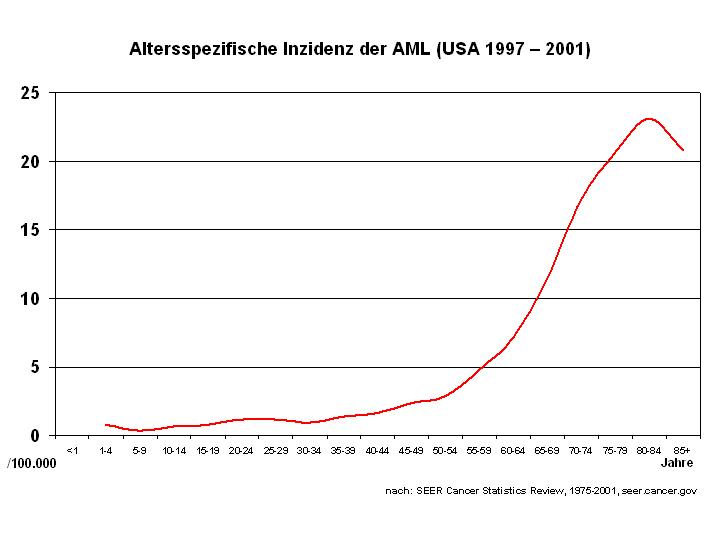
\includegraphics[width=.95\textwidth]{images/Alter_AML_2001.jpg}
\caption{Zu sehen ist die Wahrscheinlichkeit des Auftretens einer akuten myeloischen Leukämie in Abhängigkeit zum Alter. \textbf{ich suche noch nach einer aktuellen Studie}}
\label{fig:Alter_AML}
\end{figure}
Eine Leukämie kann in jeder Altersstufe auftreten, doch es gibt spezifische Altersgruppen in denen spezielle Arten der Leukämie wahrscheinlicher sind, siehe \ref{fig:Age_AML_ALL}, so treten im Kindesalter hauptsächlich akute lymphatische Leukämie (ALL) auf[Childhood acute myeloid leukaemia]. Im Erwachsenenalter hingegen ist eine AML die wahrscheinlichste Erkrankung, siehe \ref{fig:Alter_AML}.

\begin{figure}
\centering
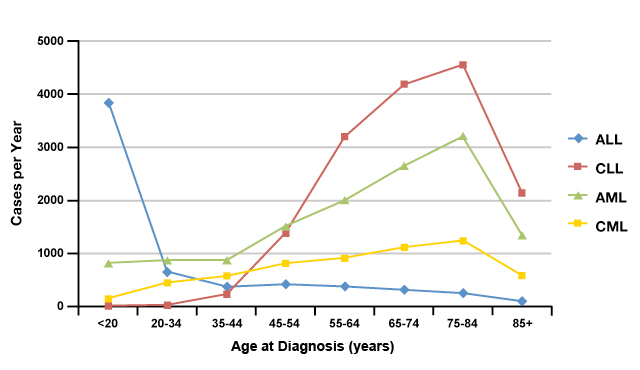
\includegraphics[width=.95\textwidth]{images/Age_AML_ALL.jpg}
\caption{Dargestellt ist die Wahrscheinlichkeit des Auftretens einer speziellen Leukämie in Abhängigkeit zum Alter. \textbf{auch hier -> aktuellen Studie kommt}}
\label{fig:Age_AML_ALL}
\end{figure}

Leukämie entsteht durch genetische Veränderungen in undifferenzierten Blutstammzellen. Wenn die Mutationen in speziellen Regionen liegen [Complex molecular genetic abnormalities in aml], so teilen sich die Zellen unkontrolliert und sind in ihrer Funktion stark eingeschränkt. Es genügt bereits eine kleine Veränderung in einer der Stammzellen, damit deren Nachkommen die gesunden Zellen verdrängen. Leider sind die Ursachen für diese genetische Modifikation im großen noch unbekannt, im allgemeinen wird jedoch vermutet, dass die spezifischen Risikofaktoren welche Krebs begünstigen auch eine Leukämie verursachen können. Durch die technische Weiterentwicklung der Länder und der damit verbundenen erhöhten Population und Lebensspanne der Menschen, steigt die Anzahl der Krebserkrankungen. Hierbei spielen Alter, Rauchen, Übergewicht, sportliche Aktivität und Reproduktionsverhalten geprägt durch die Urbanisierung eine zentrale Rolle [Global cancer statistics]. Des Weiteren ist die Aussetzung spezieller Strahlung, z.B. ionisierende Strahlung oder passive Radon Strahlung, sowie mutagene Chemikalien, diverse Viren und genetische Vorbelastung im Verdacht krebserregend zu sein.

\textbf{Behandlung? (Paper wäre gut)}
Therapie mit Zytostatika und allogene Knochenmark- bzw. Stammzelltransplantation

wie viele Menschen gehen in Remission 

Rückfallquote


%Das Ziel ist jede Mutation zuverlässig klassifizieren zu können.
%AML ist die Häufigste Erkrankung im Erwachsenen Alter
\section{Zielsetzung}

Im Universitätsklinikum Marburg in der AG Brendel wird mit dem Illumina TruSight Panel\footnote{\url{https://www.illumina.com/products/by-type/clinical-research-products/trusight-myeloid.html}} gearbeitet, um AML spezifische Regionen zu untersuchen. Dieses Panel liefert nach dem Screening eine Tabelle mit allen Mutationen des Patienten und deren Lokalisation. Auffällig dabei ist, dass die meisten Mutationen in Form von Single Nucleotide Polymorphism (SNPs) auftreten. Obwohl alle Patienten die gleichen Symptome einer AML zeigen, sind die Meisten der detektierten SNPs Patienten spezifisch und sind somit noch unbekannt und ihre Wirkung auf das entsprechende Gen kann nicht ermittelt werden. Dies hat zur Folge, dass keine Aussage über eine eventuelle Pathogenität und weiter deren Einfluss auf den Organismus getroffen werden kann.

Ziel dieser Masterarbeit ist die Entwicklung eines Programms zur Klassifizierung von SNPs aus dem \emph{Illumina TruSight Myeloid Sequencing Panel} mit Hilfe von Aminosäurerest-Pseudopotentialen.

Klassifikationen von SNPs sind eminent wichtig um ein Verständnis für die Ursachen von AML zu erhalten, doch leider haben wir in den Meisten Fällen keinerlei Informationen über die Pathogenität der gefundenen SNPs. In einer vorherigen Arbeit wurde eine Programm zum annotieren von SNPs geschrieben, jedoch liefert dieses nur einen Matthews Correlation Coefficient (MCC) von 0,66 und ist damit verbesserungswürdig, siehe Kapitel \ref{sec:sapa}. 

Nun soll der Versuch unternommen werden eine Annotation der SNPs unter Zuhilfenahme der 3d Struktur zu ermöglichen. Mittels des Modells der Aminosäurerest-Pseudopotentialen soll überprüft werden, inwiefern sich Energieprofile als Datengrundlage für eine SNP Annotation in diesem Forschungsbereich eignen. Zusätzlich soll mithilfe der PDB und Pfam diejenigen Proteinfamilien ermittelt werden, welche eine aufgeklärte Struktur in der PDB besitzen, umso durch SNPs auftretende Veränderungen der PSI \& PHI Winkel, erklären zu können. Letztendlich soll getestet werden in welcher Proteindomäne der SNP liegt, z.B. in einem hoch konservierten Bereich in einer Pfam Familie liegt, um auch hiermit eine Klassifikation vorzunehmen zu können.



\section{Aufbau der Arbeit}

Zu Beginn dieser Arbeit werden die Grundlagen vermittelt, welche für die Arbeit essentiell sind. Dies beinhaltet die Erläuterung der Theorie der Aminosäurerest-Pseudopotentiale und deren Mathematischer Hintergrund. Zudem beinhaltet ein Kapitel die Erklärung der Datenbanken \emph{PDB} und \emph{Pfam}, welche als die Grundlage der PSI \& PHI Winkel Berechnung genutzt wurden. Außerdem werden auch die Grundlagen des \emph{MCCs}, \emph{Ramachandran Plots} und \emph{Homologie Moddeling} 
%und \emph{Machine Learning}
erklärt. Abschließend wird die lokale Berechnung der Energieprofile mittels Nextflow auf dem Clusters der Bioinformatics and Systems Biology Group der Justus-Liebig-Universität Gießen, kurz vorgestellt.

Nach der Vermittlung der Grundlagen, folgt ein kurzes Kapitel zu den bisherigen Erkenntnissen aus der vorangegangenen Arbeit SAPA, als Einleitung zum Hauptteil.

Der Hauptteil der Arbeit beginnt mit der Konstruktion eines adäquaten Dantesatzes, anhand vorangegangener Arbeiten. Dabei wird vor allem auf die Selektion der Daten eingegangen und deren Nutzbarkeit auf das vorliegende Problem. Anschließend wird die Erarbeitung des Programms zur Annotation der SNPs vorgestellt.

\textbf{hier fehlen noch ein Paar Schritte}

Abschließend erfolgt die Evaluation Anhand eines ClinVar Datensatzes, welcher benigne und pathogene SNPs enthält, welche von \emph{mehreren Autoren} submittiert wurden und die \emph{gleiche Annotation} beinhalten. Nach der Evaluation werden deren Ergebnisse und die Erkenntnisse der Arbeit nochmals zusammengefasst und die Aussagekraft der Klassifikation des erstellen Programms diskutiert.



%Das geht dann so \cite{Lamport95}.
\chapter{Methoden}
%\label{cha:Metoden abkürzung}

In diesem Kapitel werden die Grundlagen vermittelt, welche für das Verständnis der Arbeit in ihrer Gänze notwendig sind.
%und Evaluation der Arbeit von Bedeutung sind.

\section{Aminosäurerest-Pseudopotentiale}

Bei den \acf{APs} handelt es sich um eine Methode der Transformation der physikochemischen und wechselwirkenden Eigenschaften der Aminosäuren der Proteinstruktur in ein Energiemaß. Diese Energiemaße werden dabei durch eine Dezimalzahl dargestellt und im Gegensatz zur hochkomplexen 3D Strukturen sind die Berechnungen mit ihnen unmittelbarer. Die Energieprofile stehen auf dem Webserver \emph{eProS}\footnote{\url{https://biosciences.hs-mittweida.de/epros/}} zum Download bereit. Zusätzlich wurde zur lokalen Berechnung und zu Testzwecken eine lokale Möglichkeit von den Entwicklern der \ac{bigM}\footnote{\url{http://www.bioforscher.de/bigM/}}, zur Berechnung der Energieprofile, zu Verfügung gestellt.

Durch die \ac{APs} können zu den lokalen Interaktionen der direkten Nachbarn, auch noch die globalen Interaktionen der indirekten Nachbarn hinzugezogen werden (Abb. \ref{fig:8A_Sphaere}). Zur Berechnung benutzt man die Betrachtung einer 8 Angström Sphäre, um die betreffende Aminosäure und analysiert ob noch andere Aminosäuren des Proteins in diese Sphäre hineinragen. Somit können auch Effekte wie sterische Hinderung berücksichtigt werden. Durch diese neue Sichtweise löst man sich von der starren Betrachtungsweise der Sequenz und der 2D Struktur, wie es bei bisherigen Vorhersage-Algorithmen war.
%
\begin{figure}
\centering
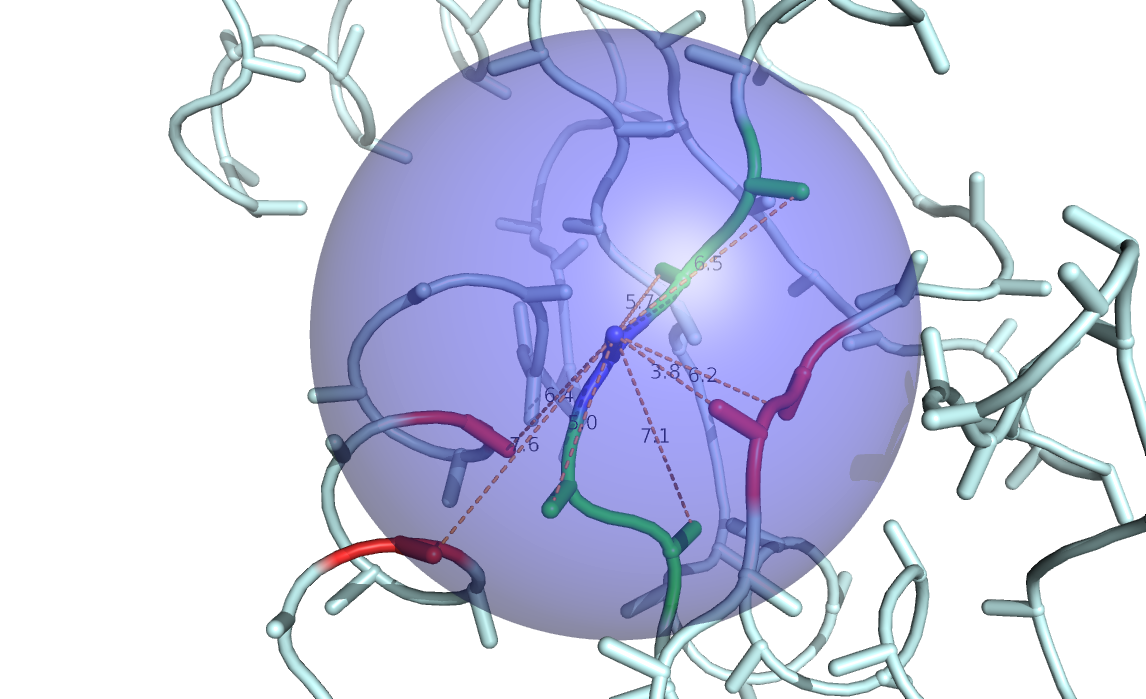
\includegraphics[width=.95\textwidth]{8A_Sphaere.png}
\caption{Ein 3D Modell einer Proteinstruktur, hellblau ist die 8 Angström Umgebung um die dunkelblaue Aminosäure im Zentrum, mit direkten Nachbarn in grün und in indirekten Nachbarn in rot. Die punktierte Linie zeigt den Abstand der $C_{\alpha}$ Atome in Angström.}%\cite{8A_Sphaere}
\label{fig:8A_Sphaere}
\end{figure}

Energieprofile sind grobkörnige Aminosäuren Interaktionsmodelle, basierend auf $C_{\alpha}$ und $C_{\beta}$ Atom Koordinaten, welche aus bekannten Protein Strukturen extrahiert wurden. Es wird die natürlich Neigung eines Aminosäurerests, mit anderen Resten zu interagieren, untersucht. Bei Membran lokalisierten Proteinen wird zusätzlich noch die Neigung der Aminosäureresten sich in Richtung der Lipid Doppelschicht zu richten, berücksichtigt. 

Generell ist die Energie abhängig von der Neigung des Aminosäurerests nach Außen ($n_{out}$) in das umgebende Milieu oder in das Innere ($n_{in}$) des Proteins. Nimmt man nun den negativen natürlichen Logarithmus zur Basis 10, so ergibt sich für $e_{a_i}$ folgende Gleichung \ref{eq:definition}:
%
\begin{equation}
  	e_{a_i} \propto -\ln{\left(\frac{n_{a_i}^{in}}{n_{a_i}^{out}}\right)}
  	\label{eq:definition}
\end{equation}

Diese Parameter sind von bekannten globularen- und membranassoziierten Proteinen hergeleitet. Wie in \ref{eq:single} zu sehen, ist die Interaktionsenergie $e_{a_{i}}$, $a_{j}$ zwischen 2 Aminosäuren $a_{i}$ und $a_{j}$ gleich die Summe der Energien der Beiden. 

\begin{equation}
  	e_{a_{i},a_{j}} = \left( e_{a_{i}} + e_{a_{j}} \right)
    \label{eq:single}
\end{equation}

Somit lässt sich die Gesamtenergie des Aminosäurerests $E_{a_i}$ mittels \ref{eq:total} berechnen:

\begin{equation}
    E_{a_{i}} = \sum_{< i, j >}{e_{a_{i},a_{j}}}
    \label{eq:total}
\end{equation}

In ihren Arbeiten hat das ePros Team Mittweida gezeigt, dass die Aminosäurerest-Pseudopotentiale genutzt werden können um die Proteinstruktur Stabilität und Funktionalität zu untersuchen. Es wurde gezeigt, dass Ähnlichkeiten der Energieprofile von Proteinen auf Ähnlichkeiten der strukturellen und funktionellen Eigenschaften dieser Proteine deuten\cite{Heinke.2011}.


\subsection{ePros Webserver}
\label{sec:epros}
Die einzige aktuelle Quelle fertig berechneter Energieprofile ist der ePros Webserver\footnote{\url{https://biosciences.hs-mittweida.de/epros}}. Mittels ePros lassen sich nicht nur Energieprofile für bestimmte \ac{PDB} IDs abrufen, sondern auch noch einige andere Tools nutzen.

\begin{figure}
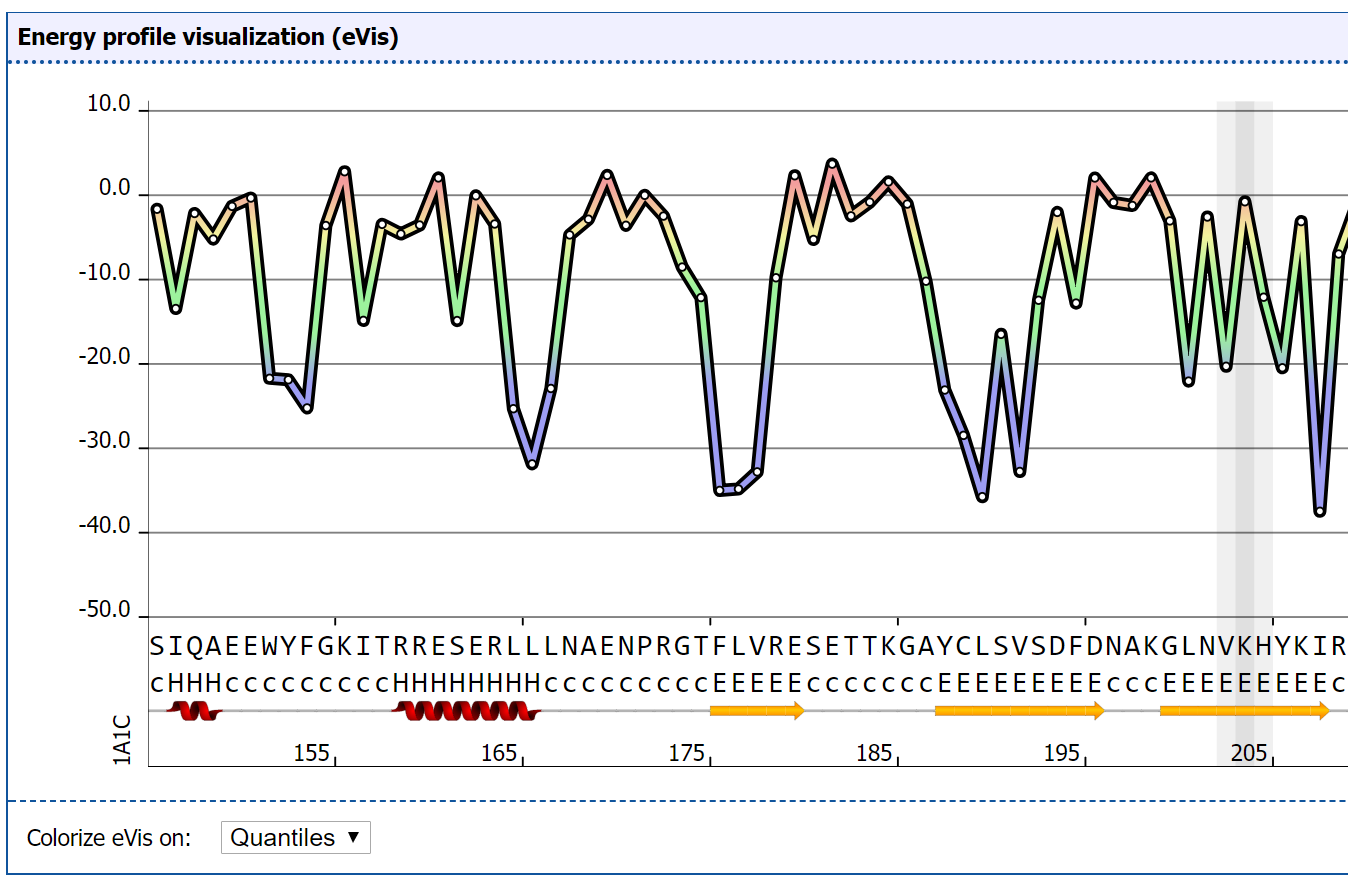
\includegraphics[width=.95\textwidth]{images/ePros.png}
\caption{Dargestellt ist ein Ausschnitt aus dem Protein \texttt{1A1C}, welches mit \ac{eVis} visualisiert wurde. Auf der Abszisse sind die Aminosäuren im Einbuchstabencode aufgetragen, siehe Tabelle \ref{tab:amino_table}. Darunter ist die Sekundärstruktur als Buchstabencode und als Visualisierung aufgetragen. Unten ist die Aminosäureposition in 10er Schritten aufgetragen. Auf der Ordinate befinden sich die Energiewerte.}
\label{fig:epros}
\end{figure}

\begin{description}
\item[eCalc]
Mittels \emph{eCalc} lassen sich Energieprofile auf Grundlage einer Struktur oder \ac{PDB} ID berechnen. Das EP wird dann in einem 2D Graphen visualisiert, sodass man leicht die Energiewerte jeder Aminosäure sehen kann, sowie deren Sekundärstruktur, siehe Abb. \ref{fig:epros}.
\item[eAlign]
Mit \emph{eAlign} ist es möglich zwei EPs mit einem modifizierten Needle-man-Wunsch/Smith-Waterman Algorithmus zu alignieren und paarweise zu vergleichen.
\item[eGOR]
Anders als \emph{eCalc} ist \emph{eGOR} ein \emph{GOR}\cite{Garnier.1996} basierter Ansatz um ein EP zu berechnen, als Grundlage dient eine Aminosäure Sequenz.
\item[eSearch]
Dieses Tool führt paarweise Vergleiche eines gegebenen EPs mit der vorberechneten eProS-Datenbank durch. Nach der Berechnung werden die besten Treffer visualisiert und können detaillierter analysiert werden.
\item[eMut]
Das besondere an \emph{eMut} ist, dass es die energetischen Ähnlichkeiten und Unterschiede von Proteinen gleicher Länge zeigt. Erkannte energetische Veränderungen könnten einen Einblick in funktionale und strukturelle Divergenzen geben.
\end{description}


\subsection{Energieprofile}
\label{sec:Energieprofil}
Energieprofile (EPs) sind die Grundlage dieser Arbeit, daher wird kurz der Aufbau des Datenformats erklärt. Ein \ac{EP} ist eine Datei mit \ac{APs} für jede Aminosäure. Im folgenden Beispiel ist das EP für die Struktur \emph{3T4F} der \emph{F Chain} dargestellt. Die ersten beiden Zeilen beschreiben das \ac{EP}, in der ersten Zeile steht der Name der Struktur und in der zweiten ob es sich um ein globuläres oder alpha helikales Protein handelt. Die restlichen Zeilen sind immer gleich aufgebaut und Tabstopp separiert. In der Spalte steht immer \texttt{ENGY}, gefolgt von dem Chain Buchstaben, dahinter steht die Aminosäurennummer und der Aminosäurennamen. Dahinter steht die Sekundärstruktur an dieser Stelle und ganz am Ende steht der Energie Wert der betreffenden Aminosäure. Am Ende der Datei kann noch \texttt{REMK} Zeilen stehen, in denen z.B. die Qualität der zugrundeliegenden \ac{PDB} Datei angegeben ist.

\begin{table}[]
\centering
\caption{Gezeigt ist ein \ac{EP} des globulären Proteins \texttt{3t4f}, zu sehen in den obersten beiden Zeilen. Die dritte Zeile enthält die Header Zeile, welche Aufschluss über die folgenden Zeilen gibt, welche immer gleich Aufgebaut sind. Die \texttt{ENGY} Zeilen beginnen mit dem Aminosäureketten Buchstaben, gefolgt von der Position, dem Namen, der Sekundärstruktur und dem Energiewert der Aminosäure.}
\label{tab:EP}
\begin{tabular}{llllll}
NAME & 3t4f &  &  &  &  \\
TYPE & globular &  &  &  &  \\
HEAD & Chain & ResNo & Res & SS & Energy \\
ENGY & F & 1 & P & c & -0.36651769255470024 \\
ENGY & F & 3 & G & c & -1.7143933253759942 \\
ENGY & F & 4 & P & c & -0.4886902567396003 \\
ENGY & F & 6 & G & c & -1.7143933253759942 \\
ENGY & F & 7 & P & c & -0.426609617950302 \\
ENGY & F & 9 & G & c & -0.8189007383286611 \\
ENGY & F & 10 & P & c & 0.8896661049247689 \\
ENGY & F & 11 & K & c & 5.678058211612121 \\
ENGY & F & 12 & G & c & 0.3188212258358888 \\
ENGY & F & 13 & E & c & 2.612350424331274 \\
ENGY & F & 15 & G & c & -1.3849755172085403 \\
ENGY & F & 16 & P & c & -0.4886902567396003 \\
ENGY & F & 18 & G & c & -1.7143933253759942 \\
ENGY & F & 19 & P & c & -0.6108628209245004 \\
ENGY & F & 21 & G & c & -1.7143933253759942 \\
ENGY & F & 22 & P & c & -0.4886902567396003 \\
ENGY & F & 24 & G & c & -0.735024098503097
\end{tabular}
\end{table}

\begin{table}[]
    \centering
    \resizebox{\linewidth}{!}{%
    \begin{tabular}{llllll}
     &  &  &  &  &  \\
     &  &  &  &  &  \\ \hline
    \multicolumn{1}{|l|}{Name} & \multicolumn{1}{l|}{Abk.} & \multicolumn{1}{l|}{Symbol} & \multicolumn{1}{l|}{Acylgruppe} & \multicolumn{1}{l|}{essentiell?} & \multicolumn{1}{l|}{Ø in Proteinen} \\ \hline
    Alanin & Ala & A & Alanyl- & nein & 9,0 \% \\
    Arginin & Arg & R & Arginyl- & semi & 4,7 \% \\
    Asparagin & Asn & N & Asparaginyl- & nein & 4,4 \% \\
    Asparaginsäure & Asp & D & $\alpha$-Aspartyl- & nein & 5,5 \% \\
    Cystein & Cys & C & Cysteinyl- & nein & 2,8 \% \\
    Glutamin & Gln & Q & Glutaminyl- & nein & 3,9 \% \\
    Glutaminsäure & Glu & E & $\alpha$-Glutamyl- & nein & 6,2 \% \\
    Glycin & Gly & G & Glycyl- & nein & 7,5 \% \\
    Histidin & His & H & Histidyl- & semi & 2,1 \% \\
    Isoleucin & Ile & I & Isoleucyl- & ja & 4,6 \% \\
    Leucin & Leu & L & Leucyl- & ja & 7,5 \% \\
    Lysin & Lys & K & Lysyl- & ja & 7,0 \% \\
    Methionin & Met & M & Methionyl- & ja & 1,7 \% \\
    Phenylalanin & Phe & F & Phenylalanyl- & ja & 3,5 \% \\
    Prolin & Pro & P & Prolyl- & nein & 4,6 \% \\
    Serin & Ser & S & Seryl- & nein & 7,1 \% \\
    Threonin & Thr & T & Threonyl- & ja & 6,0 \% \\
    Tryptophan & Trp & W & Tryptophyl- & ja & 1,1 \% \\
    Tyrosin & Tyr & Y & Tyrosyl- & nein & 3,5 \% \\
    Valin & Val & V & Valyl- & ja & 6,9 \%
    \end{tabular}}
    \caption{Die 20 kanonischen Aminosäuren mit Abkürzungen, Acylgruppe und prozentualer Anteil an der Gesamtheit\protect\footnotemark. Diese Tabelle dient dem Verständis der Tabelle \ref{tab:EP}, \ac{Abb} \ref{fig:epros}, \ref{fig:energy_ranges} und \ref{fig:ep_vs_snp}.}
    \label{tab:amino_table}
\end{table}
\footnotetext{\url{https://de.wikipedia.org/wiki/Aminosäuren##Kanonische_Aminos.C3.A4uren}}




\newpage
\section{Datenbanken}
Bei dem Aufbau eines passenden Datensatzes wurden die Datenbanken \textbf{PDB} und \textbf{Pfam} genutzt, welche zusammen als Datengrundlage für die spätere $\psi$ \& $\phi$ Winkel Kalkulation dienten. 


\subsection{RCSB PDB}

Eine wichtige Grundlage der Arbeit ist die „Protein Daten Bank“ kurz PDB\cite{Bernstein.1977}, sie enthält die 3D Strukturdaten der Proteine, welche die Grundlage der Energieprofile sind. Die \ac{PDB} enthält zusätzlich noch Strukturdaten von Nukleinsäuren und komplexen \emph{Assemblies}, die in allen Aspekten der Biomedizin und der Landwirtschaft, von der Proteinsynthese bis hin zum Gesundheitswesen von Bedeutung sind. Die \ac{PDB} bietet auf Grundlage dieser Daten Tools für Forschung und Bildung in der Molekularbiologie, in der Strukturbiologie und in der Rechenbiologie an.
Die \ac{PDB} wurde 1971 von den \ac{BNL}\footnote{\url{https://www.rcsb.org/pdb/static.do?p=general_information/about_pdb/index.html}} als Archiv für biologische makromolekulare Kristallstrukturen etabliert und beinhaltete anfangs nur 7 Strukturen. 1980 zeigte sich ein rasanter Anstieg der eingereichten Strukturen, ausgelöst durch einen verbesserten Prozess der Kristallographie, einen offeneren Datenaustausch der Wissenschaftlichen Gemeinschaft und der neuen Methode der Kernspinresonanzspektroskopie. So umfasst der Datensatz zum Zeitpunkt der vorangegangenen Arbeit 101.207 Strukturen (24. Juni 2014) und zum heutigen Zeitpunkt über 133.920 Strukturen (24 September 2017). Bei einem Wachstum von fast 10.000 Strukturen pro Jahr, macht dies die \ac{PDB} zur weltweit größten Sammlung von bekannten Proteinstrukturen.

\begin{figure}
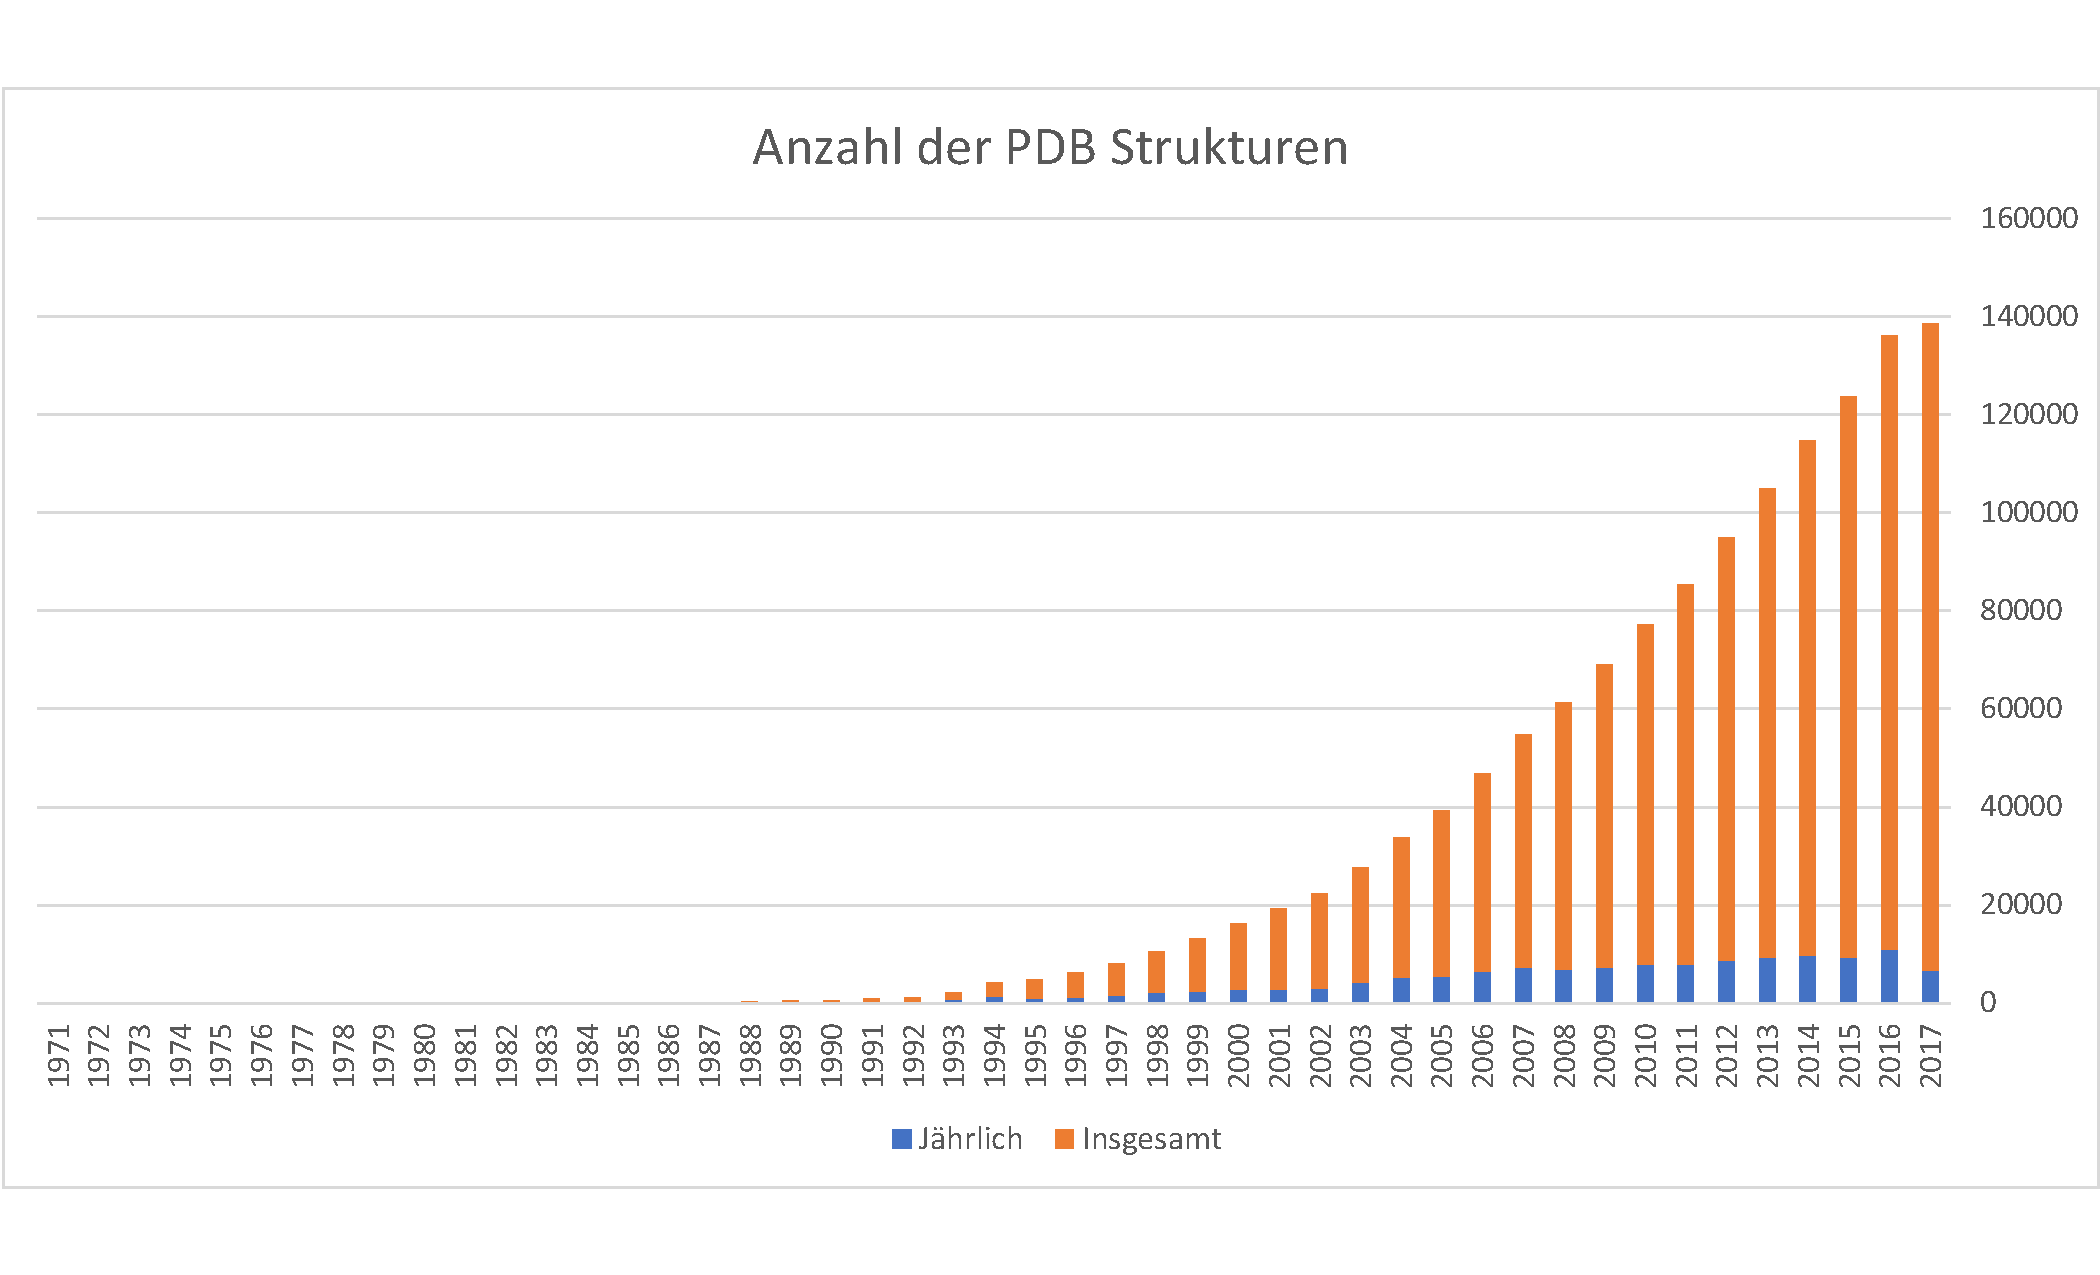
\includegraphics[width=.95\textwidth]{PDB_growth_rate.pdf}
%\caption{}
\caption{Die Jährliche Wachstumsrate\protect\footnotemark \ der \ac{PDB} seit ihrer Gründung 1971 bis 2017. Auf der Abszisse sind die Jahre aufgetragen und auf der Ordinate sind die Strukturen pro Jahr (blau) und insgesamt (orange) abgebildet.}
\label{fig:PDB_growth_rate}
\end{figure}
\footnotetext{Die Daten der Tabelle befinden sich auf der offiziellen Webseite der RCSB \ac{PDB} unter: \url{http://www.rcsb.org/pdb/statistics/contentGrowthChart.do?content=total}}

%%%%Abschnitt zu aufgebauscht!
%wen interessiert denn in deiner arbeit die nutzer. oder dass anfangs noch die daten über festplatten ausgetauscht werden musste und alles. 
%In meinen augen solltest du diesen abschnitt sehr kürzen auf das wesentliche

Der Zugriff auf die \ac{PDB} hat sich im Laufe der Jahre drastisch geändert, so wurden die Daten am Anfang noch mit Magnet Medien ausgetauscht, so kam mit der Etablierung des WWW, der Datenaustausch über dieses. Ebenso haben sich die Autoren der Daten geändert, so waren es am Anfang nur Experten auf dem Fachgebiet der Strukturellen Forschung, so sind es heute unterschiedlichste Kompetenzen in den Techniken der Röntgenkristallstrukturbestimmung, Kernspinresonanz, Kryo-Elektronenmikroskopie und theoretischen Modellierung. Genau so hat sich auch die Nutzerschaft erweitert, sodass es heute eine sehr diverse Gruppe aus Forschern, Lehrern und Studenten in den Fachbereichen Biologie, Chemie, Informatik und Physik ist. Die zunehmende Erkenntnis über den Wert der Daten und dem daraus resultierenden Verständnis der biologischen Funktion, sorgte für einen erhöhten Zustrom an Daten und erforderte einen neuen Weg die Daten zu sammeln, organisieren und zu verteilen. Im Oktober 1988 wurde das Management der \ac{PDB} Zuständig für die \ac{RCSB}. Die \ac{PDB} setzt sich heute aus einer Vielzahl von Subdatenbanken zusammen, die wichtigsten sind die Europäische \ac{PDB} (PDBe), die Japanische \ac{PDB} (PDBj), die Biological Magnetic Resonance Bank (BMRB) und die Worldwide \ac{PDB} (wwPDB). Zusammen pflegen und kuratieren diese Datenbanken die \ac{PDB} und sorgen dafür, dass die \ac{PDB} weltweit frei und öffentlich verfügbar ist.

Die Vision der RCSB ist es eine Ressource zu schaffen, welche mittels modernster Technologien, die Nutzung und Analyse von Strukturdaten erleichtert und damit eine Grundlage für die biologische Forschung stellt. 

In dieser Arbeit wurde mit dem \ac{PDB} Dateiformat gearbeitet, sodass dieses im folgenden Abschnitt erklärt wird. Alle Strukturen der \ac{PDB} sind verfügbar in dem .pdb Format, dieses ist sehr strikt geregelt, jede Zeile darf maximal 80 Zeichen enthalten und muss mit einem Identifyer beginnen. Anders als bei ähnlichen Formaten, werden hier einzelne Spalten nicht durch Tabs separiert, sondern befinden sich an genau charakterisierten Positionen. Z.B. ist der \emph{Residue name} in der \texttt{ATOM} Zeile immer an der Position 18-20 zu finden, wobei die 1. Position bei 1 beginnt und nicht bei 0. Für weitere Arbeiten ist die Seite 176 in den Formatvorgaben\footnotetext{Die Formatvorgabe ist zu finden unter \url{ftp://ftp.wwpdb.org/pub/pdb/doc/format_descriptions/Format_v33_A4.pdf}} der \ac{PDB} interessant.


\subsection{Pfam}

Die Protein Family Database\cite{Finn.2014} oder kurz Pfam enthält nah verwandte Sequenz Alignments, sogenannte Protein Familien. Diese setzen sich aus einem repräsentativen Subset aus einem Satz übereinstimmender Sequenzen zusammen, dem sogenannten „Seed Alignment“. Dieses \emph{Seed Alignment} wird anschließend genutzt um ein \emph{Profil hidden Markov model} (HMM) \cite{Soding.2005} mittels der Software HMMER\cite{Mistry.2013} zu erstellen. Nun wird das Profil HMM mit Datenbanken verglichen und um alle Sequenzen erweitert, welche über dem \emph{gathering threshold} GA liegen. GAs werden per Hand kuratiert und sind Familien spezifisch. Diese neuen Mitglieder der Familie werden an das Profil HMM aligniert um ein volles Alignment zu erzeugen. Pfam-Einträge, welche als verwandt identifiziert wurden, werden in Gruppen zusammengefasst, die als \emph{Clans} bezeichnet werden. Beziehungen werden sowohl mittels Sequenzinformationen via HMMER cross matches und SCOOP \cite{Bateman.2007}, als auch durch Protein Homologie Detektion durch HMM-HMM Vergleiche, mit HHsearch \cite{Fidler.2016} ermittelt.

Die Pfam wurde 1997 von Sonnhammer EL, Eddy SR und Durbin R. ins Leben gerufen \cite{Sonnhammer.1997}. Ihr Ziel war es eine Datenbank zur Proteinsequenz Klassifizierung und Analyse zu erschaffen. Die Pfam setzt sich aus zwei Teilen zusammen, der Pfam A und Pfam B. Die Pfam-A ist kuratiert und enthält gut charakterisierte Protein Domain Familien mit hochqualitativen Alignments. Dies wird durch manuell überprüften Seed Alignments und HMMs, gewährleistet. Pfam B hingegen enthält Sequenzfamilien, bei denen der Domainer Algorithmus zum Alignieren und Clustern aller nicht Pfam A Sequenzen, genutzt wurde. 

Die Aktuelle Version ist Pfam 31.0 und wurde am Europäischen Bioinformatik Institut (EBI)\footnote{\url{https://www.ebi.ac.uk}} produziert, mittels einer Sequenzdatenbank namens Pfamseq, welche auf UniProt\footnote{\url{http://www.uniprot.org}} basiert. Sie enthält aktuell 16712 Familien in 607 Clans (März 2017).
\begin{figure}
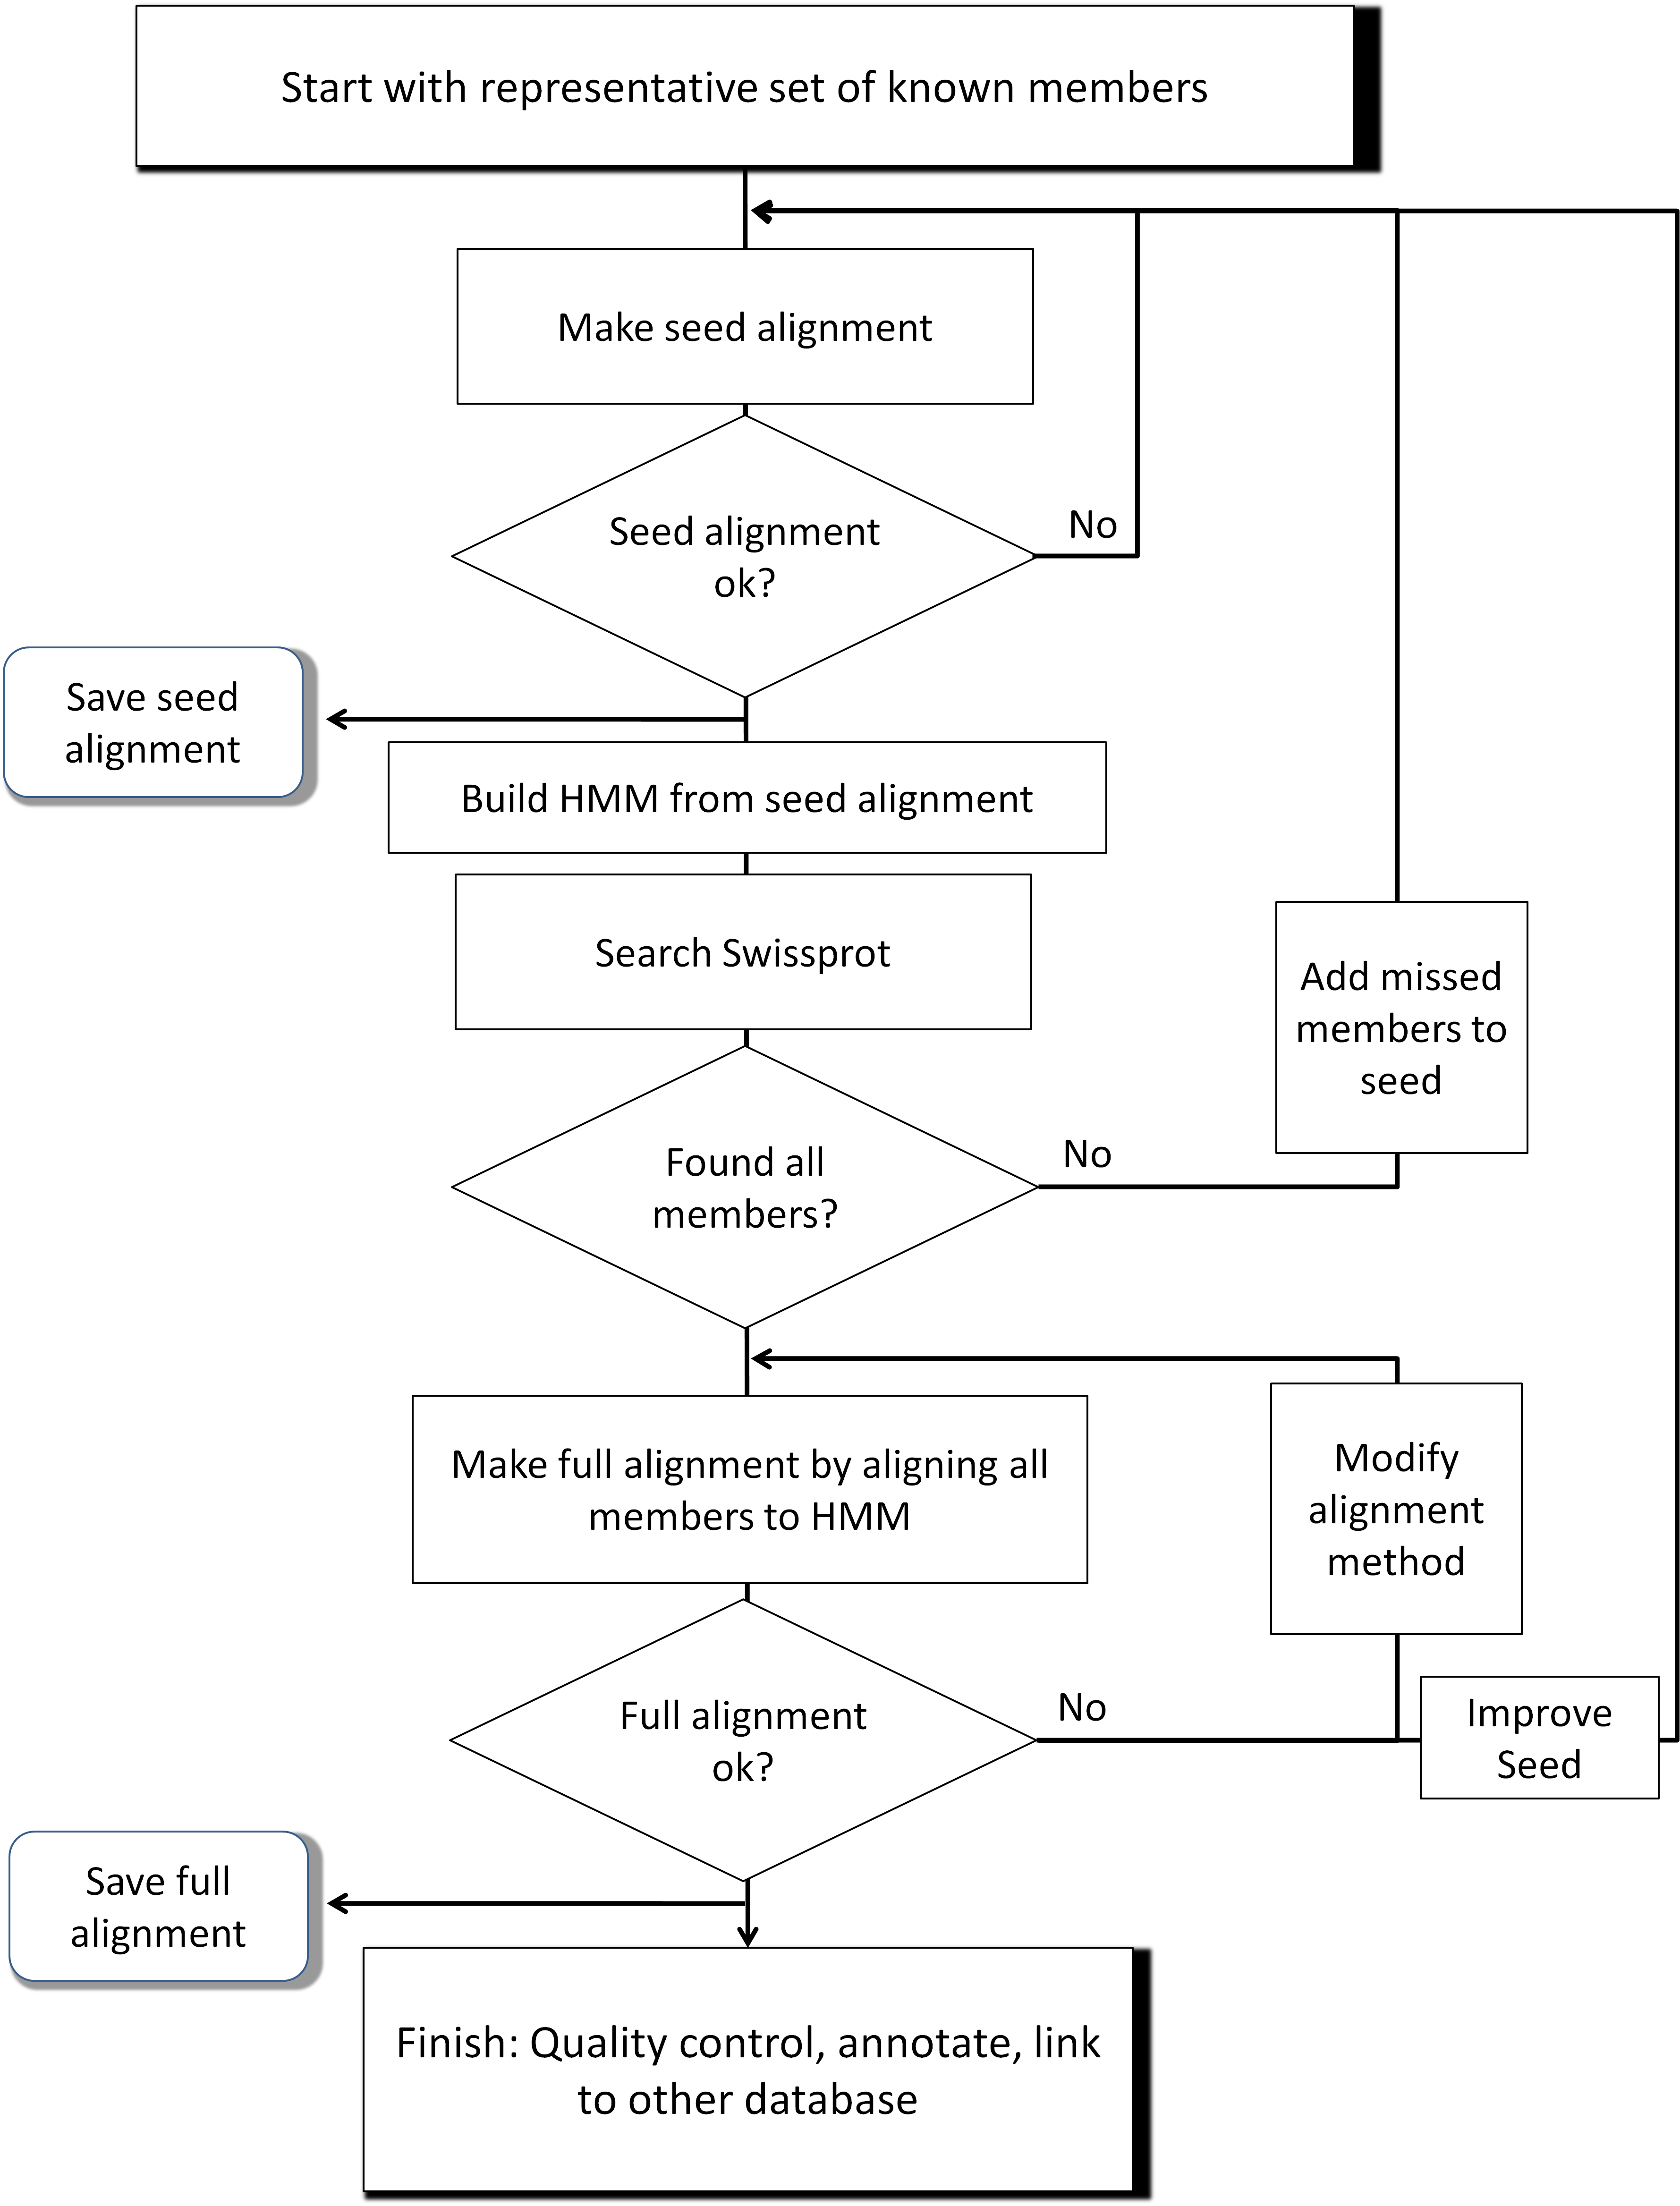
\includegraphics[width=.95\textwidth]{Pfam_workflow.png}
\caption{Abgebildet ist der \ac{Pfam} Daten Workflow, welcher die Schritte von einem repräsentativen Set bekannter Mitglieder, über das \emph{SEED} bis zum vollständigen Alignment zeigt.}
\label{fig:Pfam_workflow}
\end{figure}


\section{Bewertungen von Klassifikationen}

In dieser Arbeit war es wichtig die vorhergesagten Klassifikationen zu bewerten, dabei hängt die Güte des Klassifikators von dessen Typ ab. In diesem Fall handelt es sich um einen binären Klassifikator, daher können zwei Bewertungsverfahren in Betracht gezogen werden.

\subsection{F1 Score}
Der F1 Score ist ein statistisches Maß um die Testgenauigkeit zu bewerten. Er verwendet sowohl die \emph{Präzision} p, als auch den \emph{Recall} r um den Score zu berechnen. P ist die Anzahl aller richtigen positiven Ergebnisse, geteilt durch die Anzahl an allen positiven Ergebnissen. R ist die Anzahl an vorhergesagten richtigen positiven Ergebnissen, geteilt durch die Anzahl der tatsächlich positiven Ergebnisse (\ref{eq:f1_score}). 
\begin{equation}
    F_{1} = 2 \times \frac{1}{\frac{1}{recall}+\frac{1}{precision}} = \frac{\text{precision} \times \text{recall}}{\text{Precision} + \text{recall}}
    \label{eq:f1_score}
\end{equation}

Der F1 Score kann Werte von 0 bis 1 annehmen, wobei ein Score von 1 die beste mögliche Aussage bedeutet.


\subsection{Matthews correlation coefficient}

Der \emph{Matthews correlation coefficient}, oder kurz MCC ist ein Maß um die Qualität einer binären Klassifikation zu bewerten und wird oftmals im Bereich des \emph{Machine Learnings} angewandt. Der Biochemiker Brian W. Matthews führte diesen Algorithmus 1975, in seinem Paper „Comparison of the predicted and observed secondary structure of T4 phage lysozyme“\cite{Matthews.1975} ein. Der MCC berücksichtig \emph{true} und \emph{false postives}, sowie \emph{true} und \emph{false negatives}, um eine Bewertung einer beobachtete und vorhergesagte zwei Klassen Klassifizierung zu treffen. Dabei kann der MCC einen Wert von -1 bis 1 annehmen, ein Koeffizient von 1 repräsentiert eine perfekte Vorhersage. Ein Koeffizient von 0 bedeutet, dass die Vorhersage nicht besser ist, als ein zufälliger Münzwurf. Ein Wert vom -1 deutet auf eine totale Differenz zwischen Beobachtung und Vorhersage hin. Der MCC ist auch bekannt als Phi Koeffizient und zusammenhängend mit der chi Quadrat Statistik, für eine 2x2 Kontingenztabelle, in der n für die totale Anzahl der Beobachtungen steht.

\begin{equation}
    |MCC| = \sqrt{\frac{x^2}{n}}
    \label{eq:mcc}
\end{equation}

Der MCC gilt als ausbalanciertes Maß, selbst wenn die Klassen sehr verschiedene Größen haben, Andere Maße, wie der einfache „Anteil der richtigen Vorhersagen“, auch bekannt als statistische Genauigkeit, sind nicht besonders hilfreich, wenn zwei Klassen unterschiedlich groß sind. Denn wenn jedes Objekt dem größeren Set zugewiesen wird, so erreicht man eine Höhere Anzahl an korrekten Vorhersagen, welche statistisch gesehen allerdings wenig Aussagekraft besitzen.

Der MCC berechnet sich direkt aus der Konfusionsmatrix \ref{table:konfusionsmatrix}, mit der Formel \ref{eq:mcc2}:

\begin{table}[]
    \centering
    \resizebox{\linewidth}{!}{%
    \begin{tabular}{l|l|l|}
        \cline{2-3}
 & pathogenic SNP (tp + fn) & benign SNP (fp + tn) \\ \hline
\multicolumn{1}{|l|}{test positive (tp + fp)} & \cellcolor[HTML]{9AFF99}true positive (tp) & \cellcolor[HTML]{FFCCC9}fals positive (fp) \\ \hline
\multicolumn{1}{|l|}{test negative (fn + tn} & \cellcolor[HTML]{FFFFC7}false negative (fn) & \cellcolor[HTML]{9AFF99}true negative (tn) \\ \hline
    \end{tabular}}
        \caption{Dargestellt ist die Konfusionsmatrix.}
    \label{table:konfusionsmatrix}
\end{table}

\begin{equation}
    MCC = \frac{TP \times TN - FP \times FN}{\sqrt{(TP + FP)(TP + FN)(TN + FP)(TN + FN)}}
    \label{eq:mcc2}
\end{equation}

In Gleichung \ref{eq:mcc2} ist TP die Anzahl der \emph{true postives}, TN die Anzahl der \emph{true negatives}, FP die Anzahl der \emph{true postives} und FN die Anzahl der \emph{true negatives}. Wenn eine der 4 Summen im Teiler 0 Ergibt, so kann man den Nenner willkürlich auf 1 setzen, sodass man einen MCC von 0 erhält, dies stellt den Grenzwert der Gleichung dar.


\section{Homologie Berechnung}
\label{sec:siwssmodel}
Im Rahmen dieser Arbeit war es nötig 3D Strukturen für Protein Sequenzen zu ermitteln welche nicht oder nur teilweise aufgeklärt sind, denn Homologieberechunungen werden häufig eingesetzt wenn es keine experimentellen Daten zu einer Struktur eines Proteins gibt. 
\begin{figure}
    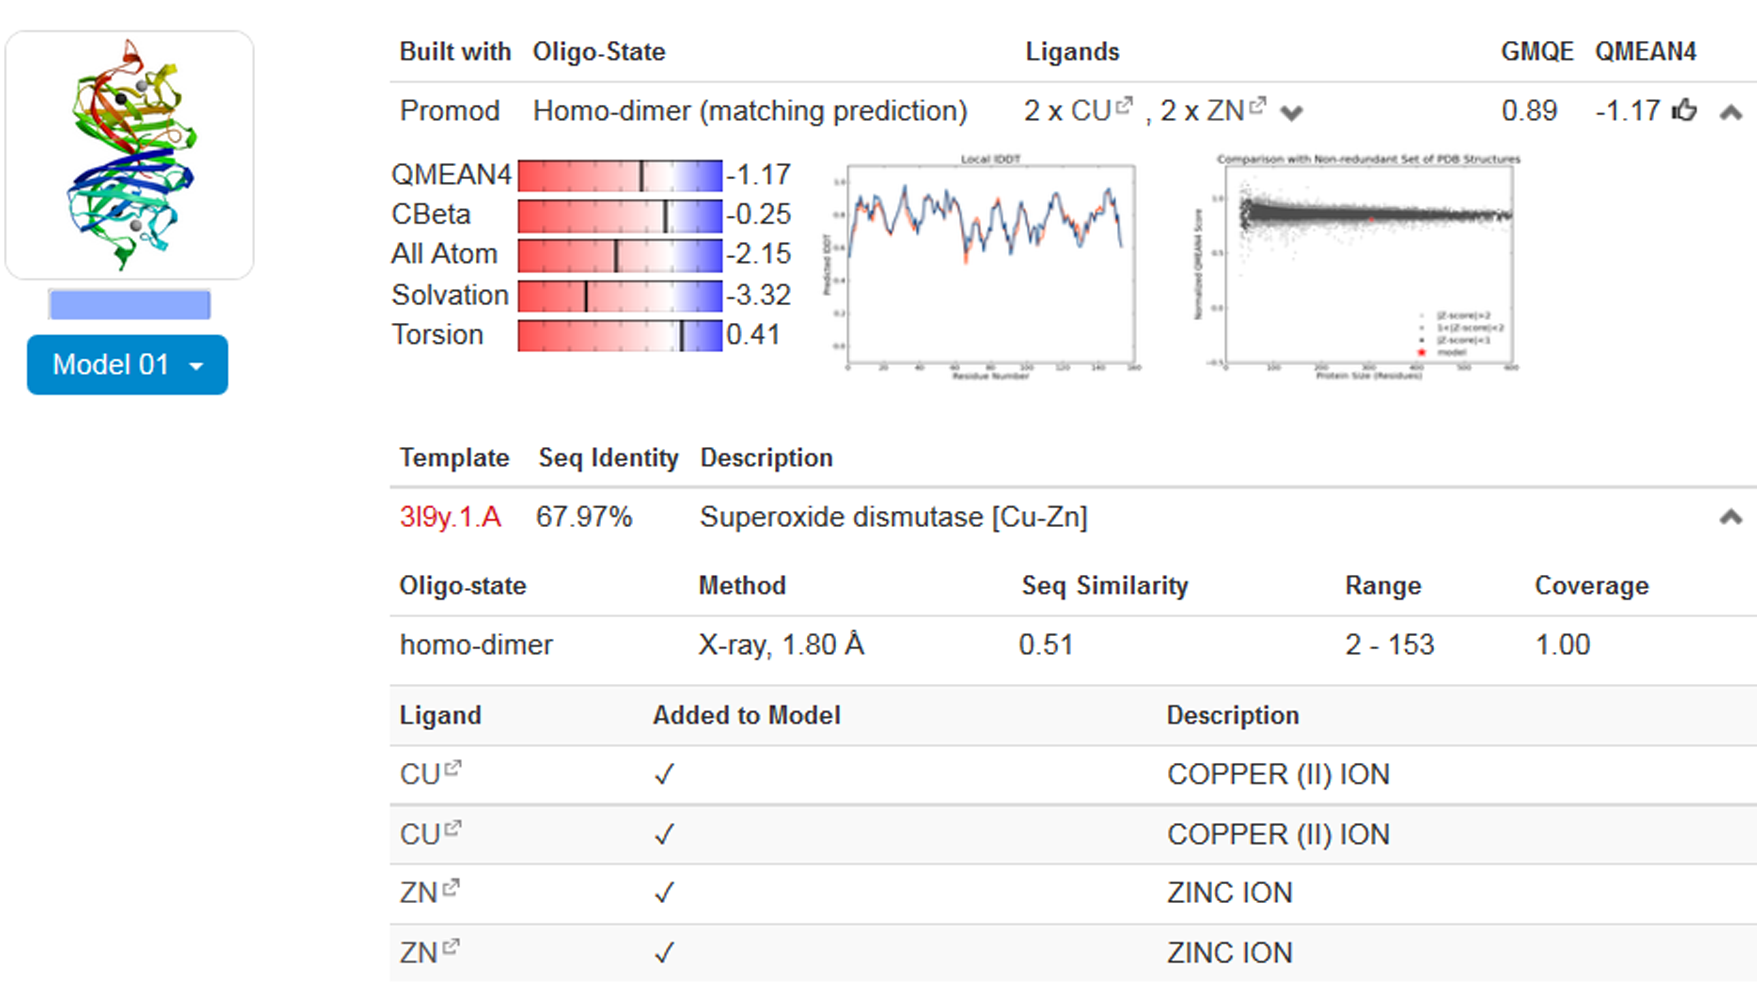
\includegraphics[width=.95\textwidth]{images/Swissmodel.png}
    \caption{Typisches Ergebnis einer Swissmodel Anfrage, für jedes Modell werden Koordinaten, Alignment, Sequenzidentität, Abdeckung, Modellierungsprotokoll, eine Qualitätsschätzung und vieles mehr, zur Verfügung gestellt.}
    \label{fig:swissmodel}
\end{figure}

\begin{quote}
    "Die Homologiemodellierung (oder vergleichende Modellierung) stützt sich auf evolutionär verwandte Strukturen (Templates) zur Generierung eines Strukturmodell eines Proteins von Interesse (Target). Der Prozess umfasst typischerweise die folgenden Schritte: (i) Vorlage Identifikation, (ii) Auswahl der Vorlagen, (iii) Modellerstellung und (iv) Schätzung der Modellqualität. Kurz gesagt, eine Bibliothek von experimentell ermittelten Proteinstrukturen wird gesucht, mit empfindlichen Sequenzsuchwerkzeugen zur Identifizierung von Proteinen die evolutionär mit dem Zielprotein verwandt sind. Wenn eine oder mehrere Vorlagen identifiziert sind, werden die Informationen der Abgleich der Ziel- und Modell-Sequenzen gemeinsam mit den 3D-Koordinaten der Vorlage (n) verwendet, um ein Strukturmodell für das Protein zu erstellen. Schließlich wird die Qualität des berechneten Modells geschätzt, um die Qualität des berechneten Modells für spätere Anwendungen zu zeigen."
\end{quote}

Übersetzt aus \cite{Biasini.2014}, den Autoren des Webservers Swissmodel\footnotetext{\url{https://swissmodel.expasy.org}}, welcher zur Homologie Berechnung genutzt wurde. 

Swissmodel zeichnet sich durch eine aufgeräumte Benutzeroberfläche, einem zuverlässig Server und einer schnellen Berechung aus, siehe \ac{Abb} \ref{fig:swissmodel}. Zudem ist kein Download erforderlich, somit werden auch keine Referenz Datenbanken benötigt. Damit war der Webserver die optimale Wahl für diese Arbeit.



\section{Ramachandran Plot}

Der Ramachandran Plot wurde 1963 von G. N. Ramachandran \cite{RAMACHANDRAN.1963} entwickelt, um die jeweiligen Diederwinkel (oder auch Torsionswinkel)  $\psi\ \&\ \phi$ eines bestimmten Protein-Backbones darzustellen. Die 3D Struktur eines Proteins wird hauptsächlich durch nicht kovalente Bindungen zwischen Atomen unterschiedlicher Aminosäurereste bestimmt, diese Bindungen sind für Strukturen wie Alpha Helices und Beta Faltblätter verantwortlich. Dies wird durch Veränderungen der  $\psi\ \&\ \phi$ Winkel des C Alpha Atoms erreicht. Denn durch den Doppelbindungscharakter der Aminosäuren ist der $\omega$ Winkel immer 180° und das Protein damit planar. Somit können sich $\psi\ \&\ \phi$ Winkel in einem Bereich von -180° bis +180° befinden, siehe \ref{fig:psi_phi}. Wenn man nun auf der Ordinate die $\psi$-, auf der Abszisse die $\phi$-Winkel der C Alpha Atome aufträgt, erhält man den typischen Ramachandran Plot. 

\begin{figure}
    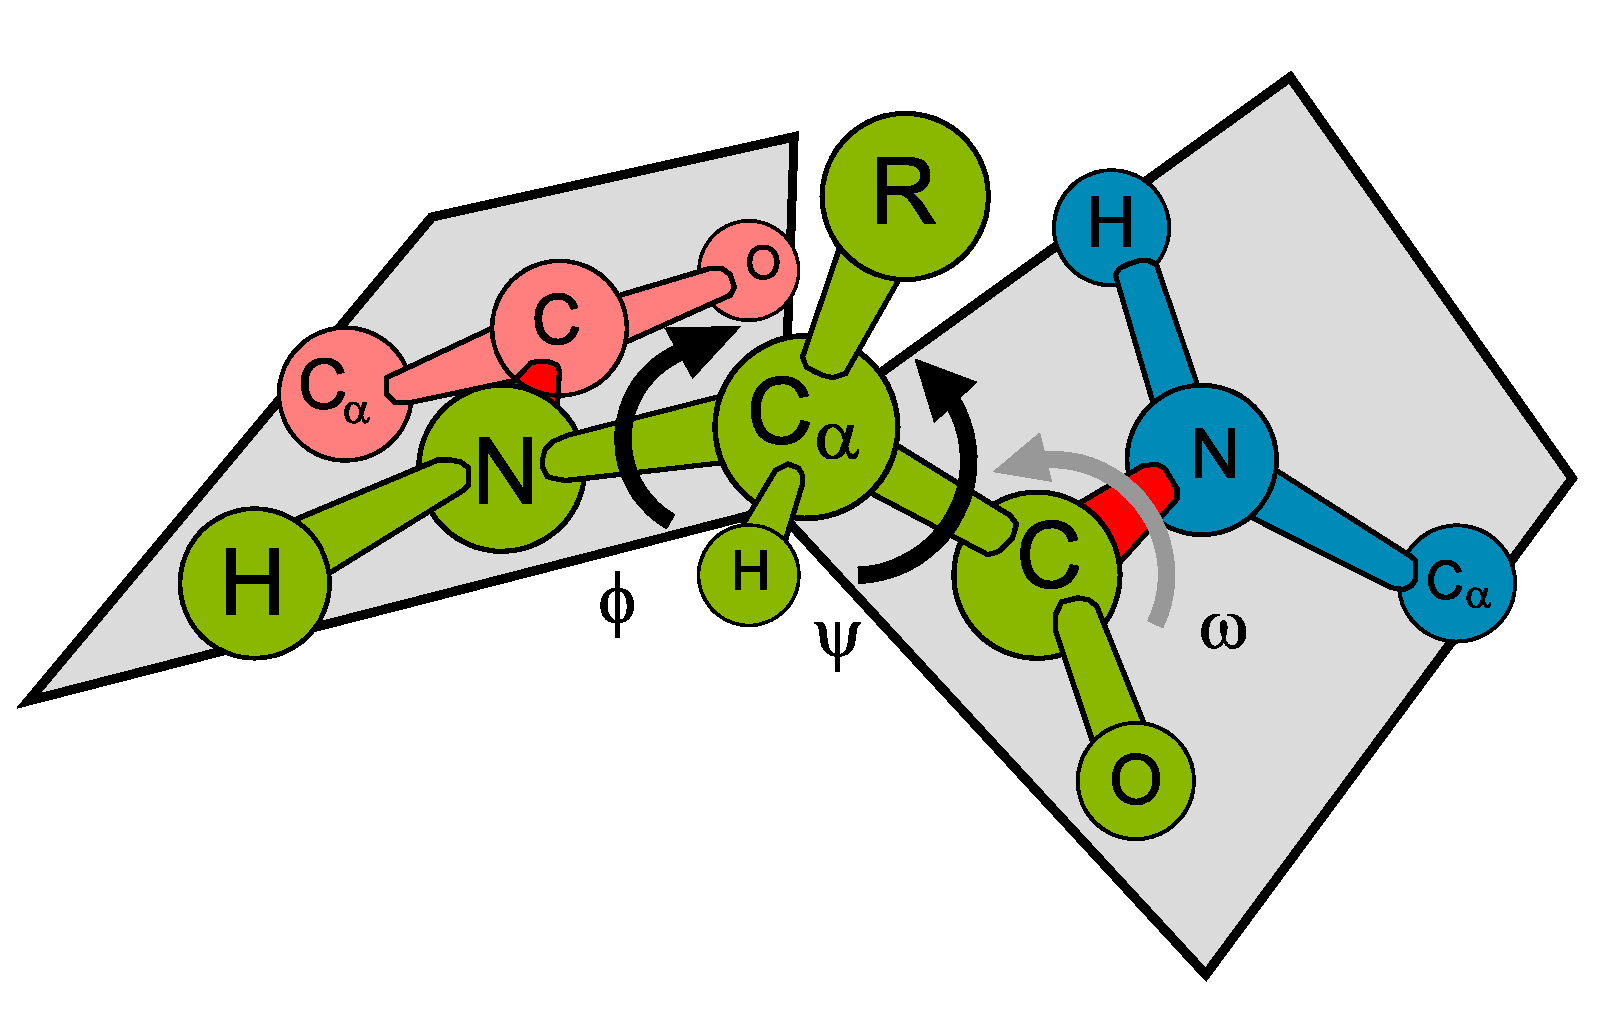
\includegraphics[width=.95\textwidth]{psi_phi.png}
    \caption{2-dimensionale Projektion eines Proteins mit C $\alpha$ Atom in der Mitte und gekennzeichneten Winkeln. Die grauen Ebenen zeigen, dass die Atome welche durch die Peptidbindung (rot) verbunden sind jeweils auf einer Ebene liegen, so kann sich der der Aminosäurerest (grün) über seine $\psi\ \&\ \phi$ Winkeln frei drehen. Die Amino-Gruppe ist blau und die Carboxyl-Gruppe ist rosa dargestellt.\protect\footnotemark}
    \label{fig:psi_phi}
\end{figure}
\footnotetext{\url{https://application.wiley-vch.de/HOME/bioinformatik/prot/Prot_1d/ueb/pepbind.png}}

Anhäufungen im Ramachandran Plot sind immer charakteristisch für spezifische Protein Sekundärstrukturen, wie z.B. alpha Helices oder beta Faltblätter. Diese sind gut zu sehen in der Abbildung \ref{fig:ramaplot}.

\begin{figure}
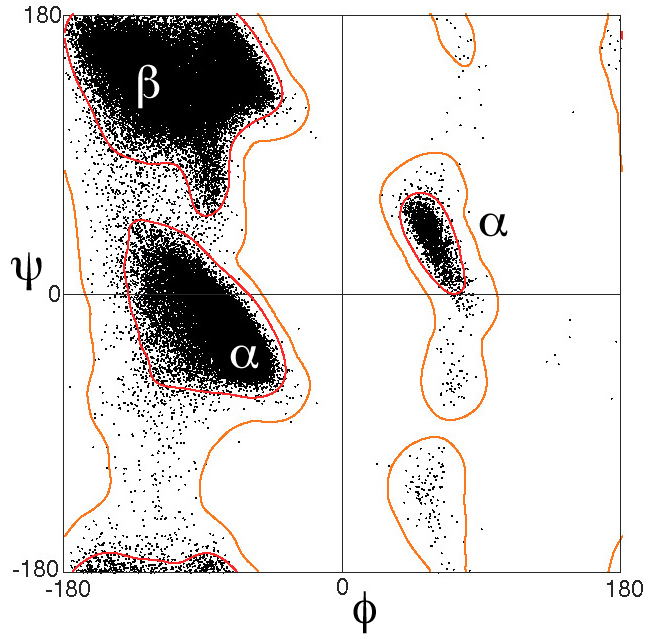
\includegraphics[width=.95\textwidth]{images/Ramaplot.png}
\caption{Abgebildet ist ein Ramachandran Plot welcher 100.000 representative Datenpunkte darstellt. Gut zu sehen sind die Akkumulationen rechts ($\alpha$) und links ($\alpha'$) drehenden alpha-Helices, sowie die beta-Faltblätter ($\beta$). Auf der Ordinate sind die PSI-, auf der Abszisse die PHI-Winkel aufgetragen\protect\footnotemark.}
\label{fig:ramaplot}
\end{figure}
\footnotetext{\url{http://proteopedia.org/wiki/index.php/Ramachandran_Plots}}

Mathematisch lässt sich der Ramachandran Plot mit folgender Gleichung beschreiben:

\begin{equation}
    f : [-\pi,\pi]\times[-\pi,\pi] \rightarrow \R_{+}
    \label{eq:rama_eq}
\end{equation}


\newpage
\section{Durchführung der Berechnungen}


\subsection{Apache Spark}
In dieser Arbeit wurde mit der Gesamten RCSB \ac{PDB} und somit mit 133.277 Energieprofilen gearbeitet, um diese Datenmasse adäquat und schnell zu verarbeiten wurde sowohl eine Hardware, als auch Software Lösung benötigt, da ein normaler PC nicht mehr ausreicht, diese Datenmengen zeitnah zu verarbeiten. Hierzu wurde als Hardwarelösung das Cluster der Arbeitsgruppe Goesmann genutzt, indem auf 5000 virtuelle Kerne mit 512GB RAM zugegriffen wurde. Als Softwarelösung wurde Apache Spark\footnote{\url{https://spark.apache.org}} eingesetzt, hierbei handelt es sich um eine gneral-purpose Cluster Software, welche über eine High Level API in Python, Scala, R und Java verfügt. Gerade die Python API war sehr hilfreich, da die Mehrzahl aller Skripte für diese Arbeit in Python geschrieben wurden. So konnte ein Python Skript erst lokal auf einem PC entwickelt und mit einem Testdatensatz überprüft werden, um es anschließend mit Spark auf dem Cluster der AG Goesmann zu deployen. Nach dem deploy verteilt Spark die Daten automatisch auf dem Cluster und fängt die Ergebnisse ab. 

\begin{figure}
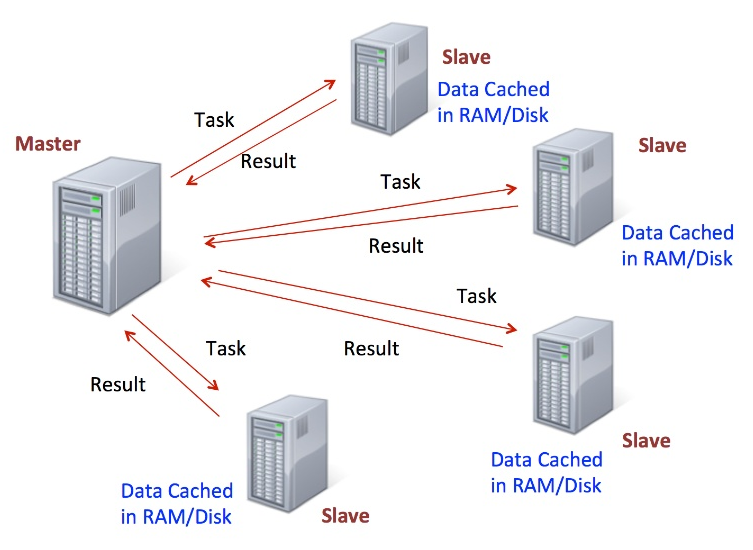
\includegraphics[width=.95\textwidth]{apache_spark.png}
\caption{Dargestellt ist die Apache Spark Job Ausführung, zwischen Master und Slave Computern im Netzwerk. Der Master verteilt Aufgaben an die Slave Rechner, welche wiederum die Ergebnisse zurück an den Master Computer senden, \ac{Abb} nach\protect\footnotemark.}
\label{fig:apache_spark}
\end{figure}
\footnotetext{\url{https://www.slideshare.net/perone/apache-spark-intro-to-largescale-recommendations-with-apache-spark-and-python}}

Zudem verfügt Spark noch über ein SQL Tool zum Verarbeiten von strukturierten Daten, MLib für Machine Learning und GraphX für Graph Prozessierung.




\newpage
\subsection{Nextflow}

\begin{wrapfigure}{R}{0.5\textwidth}
\centering
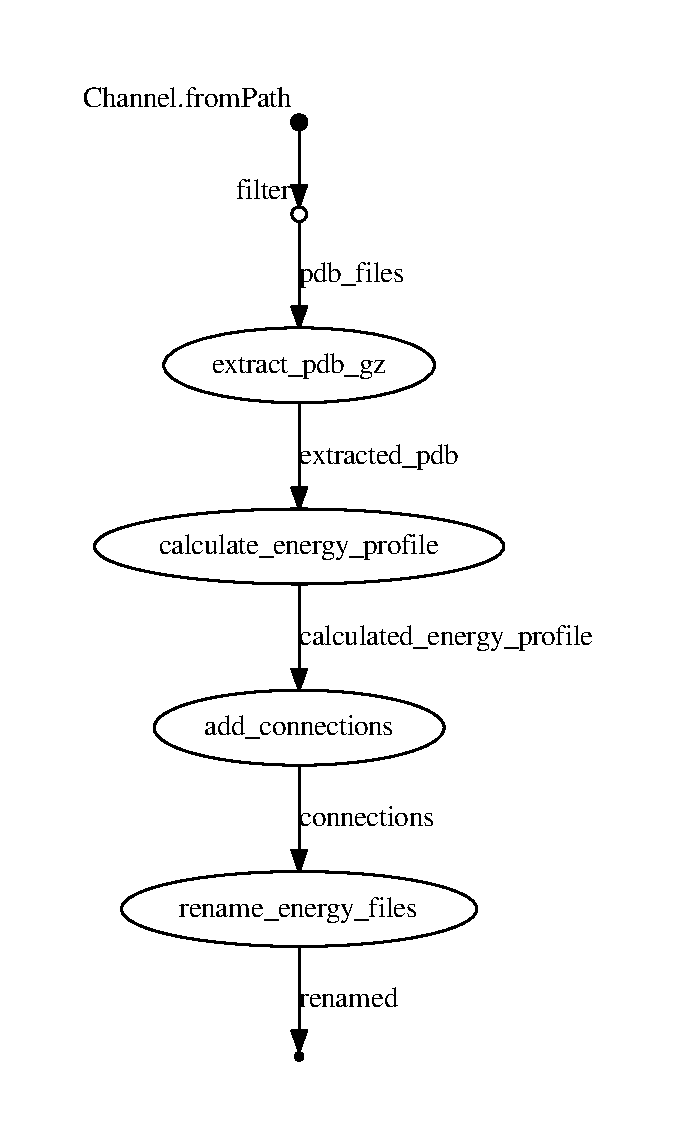
\includegraphics[width=0.45\textwidth]{images/flowchart.pdf}
\caption{Ablauf der Nextflow Pipeline dieser Arbeit, jedes Oval stellt einen Software Container dar, die Channel Namen sind an den Pfeilen zu sehen.}
\label{fig:nextflow_pipe}
\end{wrapfigure}
Bei Nextflow\footnote{\url{https://www.nextflow.io}} handelt es sich um \emph{Data-driven computational} Pipelines, mit denen man leicht Workflows parallelisieren kann. Mit Nextflow lassen sich leicht skalierbare und reproduzierbare wissenschaftliche Workflows schreiben, indem man mit Software Containern arbeitet. Der wesentliche Vorteil dieser Container ist, dass man sie in jeder beliebigen Programmiersprache schreiben kann. So wird in dieser Arbeit Nextflow verwendet um Container mit Python und Java zu vereinen. Jeder Container hat einen Eingangs- und einen Ausgangs- \emph{Channel}, also einen Fluss an Daten. Zudem kann eine Pipeline wie in \ac{Abb} \ref{fig:nextflow_pipe} dargestellt, linear ablaufen oder sich verzweigen.

Eine weitere Stärke von Nextflow ist, das man alle Pipelines nicht nur auf dem lokalen Computer ausführen kann, sondern z.B. mit \texttt{drmaa} auf einem Cluster oder in der Cloud. So lassen sich auch große Datensätze und rechenintensive Aufgaben zeitnah bewältigen.


%\textbf{Auf der Webseite stehen noch Buzzwords wie: \emph{Fast prototyping, Portable, Continuous checkpoints, Unified parallelism, Stream oriented}}



\section{Python}
Der Hauptteil der benötigten Programme dieser Arbeit wurde in Python\footnote{\url{https://www.python.org}} geschrieben. Python zeichnet sich durch eine klare und Objekt orientierte Syntax aus. Es ist vergleichbar mit Perl, Ruby, Scheme oder Java. Python gut dokumentiert und damit leicht zu lernen, dies macht es ideal für ad-hoc Programmieraufgaben und Prototyping, wie es in dieser Arbeit gefordert wurde. Außerdem läuft Python auf allen Betriebssystemen wie Mac OS X, Windows und Unix. Das vermutlich beste an Python ist, die Tatsache, dass es komplett \emph{Open Source} ist und damit Akademisch komplett entgeltfrei benutzt werden kann.

Durch meine Entwickler Tätigkeit im Edgar\cite{Yu.2017} Projekt der JLU hatte ich viel Kontakt mit Perl und der Unix Umgebung. Im privaten Rahmen setzt ich auf Windows als meinen \emph{daily driver}, damit war Python die logische Wahl, der Programmiersprache, für diese Arbeit.

In dieser Arbeit wurde die Python \emph{legacy} Version 2.7 verwendet, diese zeichnet sich dadurch aus, dass es zu diesem Zeitpunkt noch mehr Bibliotheken für diese Version gibt als für Python 3.X, was durch die fehlende Abwärtskompatibilität geschuldet ist. Denn in Python 3 wurde die Programmiersprache grundlegend überarbeitet, das hat im wesentlichen zu einem viel besseren Unicode Support, sowie eine standardmäßige \emph{bytes/Unicode} Separierung geführt. Zudem wurde die insgesamte Konsistenz der Programmiersprache verbessert.



\chapter[Datenaquirierung]{Datenaquirierung}
\label{chap:Datenaquirierung}

Dieses Kapitel befasst sich mit der Datenaquirierung, es sollte zum beginn der Arbeit der Versuch unternommen werden die Substitutionsmatrix unter Zuhilfenahme der neuen Strukturen in der \ac{PDB} neu zu berechnen. Da sich zum Zeitpunkt der Arbeit \cite{Mathias.2014} in der \ac{PDB} 101.539 Proteinstrukturen befanden und nun zum Zeitpunkt dieser Arbeit 132.095 (Oktober 2017). Dies bedeutet eine Informationserweiterung von ~30\%. Doch leider war es aus zeitlichen Gründen für mich nicht möglich die Substitutionsmatrix zu reproduzieren. Dennoch wurden die Daten als Grundlage für die $\psi$ \& $\phi$ Berechnung genutzt. Hier wurde besonderen Wert auf die Reproduzierbarkeit gelegt und Schritt für Schritt erklärt wie der Datensatz entstanden ist.



\section{Konstruktion des Datensatzes}
\label{sec:konst}

Um die Änderungen der $\psi$ \& $\phi$ in der 3D Struktur interpretieren zu können musste als erstes ein geeigneter Datensatz erstellt werden. Hierfür wurde an Hand der Arbeit \cite{Mathias.2014}, ein repräsentativer Datensatz aus der \ac{Pfam} und \ac{PDB} erzeugt, alle benutzten Skripte sind im Ordner \texttt{data\_mining} zu finden. 

%Hier sollte noch ein bisschen mehr stehen ;)
% im sinne von warum machen ich das?

\begin{enumerate}
\item
    \begin{sloppypar}
    Um schnell und effizient mit den beiden Datenbanken zu arbeiten, wurden diese von deren offiziellen Webseiten heruntergeladen. Die \ac{PDB} ist unter \url{http://www.rcsb.org/pdb/static.do?p=download/http/index.html} erreichbar und wurde via Kommandozeile mit \texttt{wget -N \url{ftp://ftp.wwpdb.org/pub/pdb/data/structures/all/pdb/*}} heruntergeladen. Die \ac{Pfam} ist zu finden unter \url{ftp://ftp.ebi.ac.uk/pub/databases/Pfam/releases/Pfam31.0/} hier wurde die Datei \texttt{Pfam-A.full.ncbi.gz} herunter geladen. Nach dem Download umfassten die Dateien der \ac{PDB} 16GB und die \ac{Pfam} 28GB (hierbei ist zu beachten das die entpackte \ac{Pfam} 212GB und die \ac{PDB} Dateien 100GB umfassen).
    \end{sloppypar}
\item
    Alle \ac{Pfams} werden in einer einzigen großen Datei zu Verfügung gestellt. Dies ist für die weitere Arbeit ungeeignet, da die gesamte Datei immer wieder in den \ac{RAM} geladen werden müsste. Der Aufbau der Dateistruktur ermöglicht es uns jedoch jeden Eintrag einer Familie separat zu erfassen und in eine Datei zu extrahieren, dies wurde mit \texttt{extract\_protein\_families.py} durchgeführt.
\item
    Um die benötigten Strukturdaten aus der PDB zu extrahieren, wird eine Datei benötigt, welche von der Pfam bereitgestellt wird. Die \texttt{pdbmap} enthält mapping Informationen, zu allen Sequenzen von Proteindomänen der \ac{Pfam}, zu denen eine Struktur auf der \ac{PDB} vorhanden ist. Durch die entsprechende Kennzeichnung durch \ac{Pfam} ID und \ac{PDB} ID, sowie Start und Ende der Proteindomäne innerhalb der gesamten Proteinstruktur, lassen sich die benötigten Strukturdaten extrahieren. Jedoch muss diese Liste vor ihrer Verwendung noch überprüft werden.
    \begin{enumerate}
        \item 
        Es ist wichtig alpha helicale Membranproteine herauszufiltern, da diese sich fundamental in ihren strukturellen Eigenschaften von globulären Proteinen unterscheiden. Dies wurde mit Hilfe des Skriptes \texttt{filter\_membrane\_protein\_ids.py} durchgeführt. Dieses Skript benötigt zusätzlich noch die Liste aller Transmembranproteine \texttt{pdbtm\_all.list.txt}, welches auf der Webseite der \ac{PDBTM} \url{http://pdbtm.enzim.hu} zu finden ist.
        \item
        Danach kann mit der Filterung der \ac{Pfams} begonnen werden, hierfür wurde das Skript \texttt{filter\_membrane\_pfams.py} verwendet.
    \end{enumerate}
\item
    Im letzten Schritt werden alle Familien Dateien herausgefiltert, zu denen mindestens eine Struktur in der \ac{PDB} vorhanden ist, Von diesen Familien wird dann nur die Sequenzen übernommen, welche eine bekannte Struktur haben. Um dieses Sequenzen zu Identifizieren mussten zwei zusätzliche Schritte durchgeführt werden.
    \begin{enumerate}
        \item
        Als erstes wurden alle \texttt{UniProtKB} AC/IDs aus der \texttt{pdbmap} mittels dem Skript \texttt{extract\_pdbmap\_ids.py} in ID Listen geparst. 
        \item
        Danach wurden diese ID Listen mit den \texttt{UniProtKB} AC/IDs auf der Webseite \url{http://www.uniprot.org/uploadlists/} eingefügt um so die korrespondierenden \texttt{EMBL} CDS IDs zu bekommen, welche die Sequenzen in den Pfams eindeutig beschreiben.
        \item
        Mit den EMBL CDS IDs war es nun möglich alle benötigten Sequenzen aus den Pfams mittels dem Skript \texttt{find\-\_pfam\-\_pdb\-\_sequences.py} zu filtern.
        \item
        Zuletzt wurde noch mit dem Skript \texttt{find\-\_empty\-\_pfams.py} alle Proteinfamilien, welche keine Sequenzen mehr beinhalten, verworfen. 
    \end{enumerate}
\end{enumerate}

Nach allen Schritten wurde so ein Datensatz erzeugt, welcher 73410 Sequenzen aus 5023 \ac{Pfams} beinhaltet, welche alle eine komplette oder partielle aufgeklärte 3D Struktur in der \ac{PDB} besitzen.

%%%% später geht es hier noch weiter %%%%%%%%%%



\section{Berechnung der Energieprofile}
\label{sec:calc_ep}
Der folgende Abschnitt befasst sich mit der Erstellung der \acf{EP}, denn ursprünglich war es geplant die \ac{EPs}  vom Webserver ePros \ref{sec:epros} herunter zu laden, doch leider waren die Downloadlinks zum Zeitpunkt dieser Arbeit nicht erreichbar. Nach einer erfolgreichen E-Mail Korrespondenz wurde ein Java Programm von der Arbeitsgruppe \emph{bigM} zu Verfügung gestellt. Mit diesem Programm war es nun möglich sowohl globuläre, als auch alpha helicale \ac{EPs}  lokal zu berechnen. 

Die Datengrundlage für \ac{EPs} ist die Struktur der Proteine welche in der \ac{PDB} gespeichert sind. Die \ac{PDB} weist zum Zeitpunkt dieser Arbeit (Oktober 2017) 132095 Strukturen vor, auf dem Webserver ePros befinden sich jedoch 346365 \ac{EPs}. Dies ist dem Umstand geschuldet, dass auf dem ePros Webserver für jede \emph{side chain} eines Proteins ein extra \ac{EP} angelegt wurde. So gibt es zum Beispiel für den \ac{PDB} Eintrag 1A0A drei \ac{EPs}, neben der Datei \texttt{1A0A.ep2}, welche alle \emph{side chains} enthält, noch \texttt{1A0A-A.ep2} und \texttt{1A0A-B.ep2}, welche jeweils nur entweder die A oder B \emph{side chain} enthalten.

Die Rechenleistung eines einzelnen PCs stellte sich allerdings als nicht ausreichend heraus um das Problem zeitnah zu lösen. Aufgrund dessen wurde ein Nextflow Pipeline geschrieben mit dem die Berechnung der \ac{EPs}  parallelisiert wurde. Somit konnte die Geschwindigkeit um den Faktor 100 gesteigert werden. Zudem wurde die Nextflow Pipeline noch genutzt um direkt die Anpassung der Daten vorzunehmen, insgesamt wurden 4 Schritte von der Pipeline ausgeführt:

\begin{enumerate}
    \item
        Als erstes wurden alle komprimierten \ac{PDB} Dateien \ac{otf} entpackt und für jede Datei ein extra Thread angelegt, mit einer maximalen Parallelisierung von 200 Threads.
    \item 
        Danach wurden die \ac{EPs}  mittels dem bereitgestellten Java Programm aus den \ac{PDB} Dateien berechnet.
    \item
        Im 3. Schritt wurde jedem \ac{EP} ein zusätzliches Verbindungsprofil hinzugefügt, indem nach benachbarten Aminosäuren innerhalb der 8 Angström Sphäre gesucht wurde, diese Kontaktmatrix ist in Abschnitt \ref{sec:Kontaktmatrix} näher erklärt.
    \item
        Im letzten Schritt wurden die Namen der Dateien bereinigt, denn Nextflow arbeitet mit vielen Dateiendungen um die Daten zu verarbeiten. Am Ende des Workflows ist der Ordner gefüllt mit \texttt{pdb*.\-ent.\-ep2.\-cnn} Dateien, diese werden nun geöffnet und anhand ihrer \ac{PDB} ID umbenannt.
\end{enumerate}

\paragraph{Hinweis:} Hierbei ist noch zu erwähnen das die Pipeline insgesamt zwei mal ausgeführt wurde, einmal mit allen globulär assozierten \ac{PDB} Daten und einmal mit allen alpha helicalen Membran Dateien, da sich die Berechnung dieser beiden Klassen unterscheidet.

Nach der Abschluss der Berechnung waren 132.098 globuläre und 3.172 alpha helicale \ac{EPs} vorhanden.

\section{Kontaktmatrix}
\label{sec:Kontaktmatrix}
Die Kontaktmatrix wurde erstellt mit dem Ziel den Energieprofil zusätzliche Informationen hinzuzufügen, ohne es dabei zu verändern oder externe Daten zu benötigen. Ein \ac{EP} mit Kontakten ist identisch zu einem \ac{EP} ohne diese (siehe Abschnitt \ref{sec:Energieprofil}), es wurde lediglich um eine Spalte, bestehend aus einem Array, aus \texttt{1} oder \texttt{0} erweitert:

\begin{lstlisting}
NAME	3t4f
TYPE	globular
HEAD	Chain	ResNo	Res	SS	Energy
ENGY	F	1	P	c	-0.3665176925547002	1 1 1 0 0 0 0 0 0 0 0 0 0 0 0 0 0
ENGY	F	3	G	c	-1.7143933253759942	1 1 1 1 1 0 0 0 0 0 0 0 0 0 0 0 0
ENGY	F	4	P	c	-0.4886902567396003	1 1 1 1 0 0 0 0 0 0 0 0 0 0 0 0 0
ENGY	F	6	G	c	-1.7143933253759942	0 1 1 1 1 1 0 1 0 0 0 0 0 0 0 0 0
ENGY	F	7	P	c	-0.426609617950302	0 1 0 1 1 1 1 1 0 0 0 0 0 0 0 0 0
ENGY	F	9	G	c	-0.8189007383286611	0 0 0 1 1 1 1 1 1 0 1 0 1 1 1 1 0
ENGY	F	10	P	c	0.889666104924768	0 0 0 0 1 1 1 1 1 1 1 1 1 1 1 1 1
ENGY	F	11	K	c	5.678058211612121	0 0 0 1 1 1 1 1 1 1 1 0 1 1 1 1 0
ENGY	F	12	G	c	0.318821225835888	0 0 0 0 0 1 1 1 1 1 1 1 1 1 1 1 1
ENGY	F	13	E	c	2.612350424331274	0 0 0 0 0 0 1 1 1 1 1 1 1 1 1 1 1
ENGY	F	15	G	c	-1.3849755172085403	0 0 0 0 0 1 1 1 1 1 1 1 1 1 1 1 1
ENGY	F	16	P	c	-0.4886902567396003	0 0 0 0 0 0 1 0 1 1 1 1 1 1 1 1 1
ENGY	F	18	G	c	-1.7143933253759942	0 0 0 0 0 1 1 1 1 1 1 1 1 1 1 1 1
ENGY	F	19	P	c	-0.6108628209245004	0 0 0 0 0 1 1 1 1 1 1 1 1 1 1 1 1
ENGY	F	21	G	c	-1.7143933253759942	0 0 0 0 0 1 1 1 1 1 1 1 1 1 1 1 1
ENGY	F	22	P	c	-0.4886902567396003	0 0 0 0 0 1 1 1 1 1 1 1 1 1 1 1 1
ENGY	F	24	G	c	-0.735024098503097	0 0 0 0 0 0 1 0 1 1 1 1 1 1 1 1 1
\end{lstlisting}

In diesem Array, ist die Information zu den benachbarten Aminosäuren gespeichert. Die Länge des Arrays ist immer gleich der Länge der Sequenz der Polypeptidkette im EP. Hierbei ist zu beachten, dass fehlende 3D Informationen und somit fehlende Aminosäuren übersprungen werden. Im obigen Beispiel sieht man dies sehr gut, die \texttt{F Chain} hat 24 Aminosäuren, doch es sind nur die 3D Positionen von 17 Aminosäuren bekannt, weswegen auch die Kontaktliste nur 17 Einträge aufweist. Iteriert man nun über das Array, so ist der erste Eintrag gleich der ersten Position in der Chain, der zweite Eintrag im Array ist hingegen der dritte in der Chain, da die Position der zweiten Aminosäure noch nicht aufgeklärt ist und somit auch im \ac{EP} fehlt.

Eine \texttt{1} bedeutet, es gibt in der 8 Angström Umgebung um die Aminosäure einen Kontakt mit der anderen Aminosäure. Am Beispiel der ersten Aminosäure Prolin an Position 1, kann man also sehen, dass diese Kontakte mit Glycin an Position 3 und Prolin an Position 4 in der Chain hat. Eine \texttt{0} bedeutet im Gegensatz es besteht kein Kontakt in der 8\AA\ Umgebung.

Um ein Kontaktprofil zu errechnen wird das Python Skript \texttt{add\-\_aa\-\_connections.py} verwendet. Zuerst wird für das jeweilige \ac{EP} die entsprechende \ac{PDB} Datei herausgesucht, in dem oben genannten Beispiel wäre dies \texttt{pdb3t4f.ent}. Nun wird über die \ac{PDB} Datei iteriert und alle Positionen der Aminosäuren analysiert und mit der Abstandsgleichung \ref{eq:abstand}, der Abstand der einzelnen Aminosäuren zueinander bestimmt.

\begin{equation}
    d=\sqrt{(x_2-x_1)^2+(y_2-y_1)^2+(z_2-z_1)^2}
    \label{eq:abstand}
\end{equation}

Es gilt:

\begin{equation}
    d = 8\text{\AA}
    \label{eq:8a}
\end{equation}

Ist \ref{eq:8a} erfüllt, so wird eine \texttt{1} in der Kontaktliste gespeichert ansonsten eine \texttt{0}, die Kontaktliste wird nun in einem \emph{dictionary} mit der Position als \emph{key} gespeichert. Wenn über alle Positionen iteriert wurde, wird nun das Energieprofil geöffnet und um die Kontaktdaten im \emph{dictionary} erweitert.





\chapter{Durchführung}
\label{chap:durchfuerung}

Ausgehend von dem nun verfügbaren Datensatz, ist es möglich mit der Anwendung auf unser Problem zu beginnen.



\section{Aminosäurerest-Pseudopotential Spektrum}


\subsection{Quantil Berechnung}

Zuerst wurde die allgemeine Verteilung der \ac{APs} in Quartile erfasst. Dies wurde mit dem Skript \texttt{check\_energy\_quants.py} durchgeführt. Dafür wurde zuerst über den Ordner mit allen globulären \ac{EP}s iteriert und alle Energiewerte in eine Liste geschrieben. Danach wurde diese Liste sortiert und mit dem Grubbs-Test \cite{Jain.2010} (alpha=0.05), wurden die Ausreißer entfernt. Abschließend wurde die Länge der Liste ermittelt und die Quartile ausgegeben.

Die oben genannten Schritte wurden für den Ordner mit den membranassoziierten Proteinen wiederholt. Die Ergebnisse wurden in eine Excel Tabelle überführt und sind in \ac{Abb} \ref{fig:quartiles_glob} und \ac{Abb} \ref{fig:quartiles_memb} dargestellt.


\subsection{Berechnungen für alle Aminosäurespektren}
Nachdem die insgesamte Verteilung der Energiewerte bekannt ist, wurde in einem weiteren Schritt überprüft, ob und wie sich die \ac{AP} Verteilung zwischen den einzelnen Aminosäuren unterscheidet. Dafür wurde der gesamte Datensatz aus 132.098 globulären \ac{EP}s mit dem Skript \texttt{check\_aa\_energy\_range.py} analysiert. 

Das Skript iteriert über die \ac{EP}s und speichert die Energiewerte, mit dem zugehörigen Aminosäurenamen, in einem Python \emph{Dictionary}. Dies ermöglicht es, über jeden \emph{Key} zu iterieren, um so nur für die gerade betrachtete Aminosäure alle Energiewerte zu verarbeiten. Nun wird für jede Aminosäure separat ein Test auf Normalverteilung aus dem Python Packet \emph{scipy}\footnote{\url{https://docs.scipy.org/doc/scipy/reference/generated/scipy.stats.mstats.normaltest.html}} durchgeführt und mittels dem Grubbs-Test die Ausreißer entfernt. Die Ergebnisse wurden abschließend mit \emph{Seaborn}\footnote{\url{http://seaborn.pydata.org}} visualisiert und sind in \ac{Abb} \ref{fig:energy_ranges} dargestellt. 

Zusätzlich wurde mit dem Skript noch ein Histogramm für jede Aminosäure erstellt, siehe \ac{Abb} \ref{fig:ep_as_distr}.



\section{SNP Analysen mittels EPs}
\label{sec:snp_analyse}

Um eine Aussage über die eventuelle Pathogenität von \ac{SNP}s zu treffen, war es erforderlich geeignete \ac{SNP}s zu finden, die betreffenden Gene zu identifizieren und eine \ac{PDB} Datei mit den Strukturinformationen des betreffenden Proteins zu generieren. Dies ist notwendig, um anschließend das \ac{EP} für die generierten \ac{PDB} Dateien zu berechnen, damit die \ac{EP}s verglichen und ausgewertet werden können.


\subsection{Identifizierung der SNPs}
\label{sec:clinvar_filter}
Um geeignete \ac{SNP}s für eine aussagekräftige Analyse zu finden, wurde auf die Datenbank ClinVar (Kapitel \ref{sec:clinvar}) zurückgegriffen.

Jedoch konnte nicht ohne Weiteres aus diesem Datensatz geschöpft werden, denn viele Variationen enthalten widersprüchliche Annotationen. Aufgrund dessen wurde auf die besten Annotationen zurückgegriffen, da fast keine \ac{SNP}s (23) in die beste Kategorie (vier Sterne) fallen, wurden zuerst nur Variationen betrachtet, welche aus dem \emph{expert panel} (drei Sterne) kommen. 

Das \emph{expert panel} enthält 5.437 pathogene und 2.878 gutartige Variationen. Von diesen waren 1.717 pathogene und 2.697 gutartige \ac{SNP}s für diese Arbeit von Interesse, da die anderen genetischen Variationen aus Deletionen, Duplikationen und Insertionen bestehen. Ausgehend von diesen \ac{SNP}s wurden alle Gene ausgewählt, welche mindestens 10 Pathogene \ac{SNP}s in der ClinVar besitzen. So wurden 6 Gene ausgewählt, die Aminosäuresequenz aus der NCBI Protein Datenbank\footnote{\url{https://www.ncbi.nlm.nih.gov/protein/}} heruntergeladen und für jeden \ac{SNP} eine entsprechende Sequenz angelegt. 

Da dieser Datensatz nach dem ersten Filterschritt immer noch zu wenige Gene und \ac{SNP}s umfasst, wurden die Kriterien der \ac{SNP} Auswahl erweitert. So wurden in einem zweiten Durchlauf auch jene \ac{SNP}s hinzugezogen, welche nicht im \emph{expert Panel} waren, sondern lediglich von mehreren Autoren eingetragen wurden. Somit standen 3.826 pathogene und 19.070 gutartige \ac{SNP}s zur Verfügung. Zusätzlich wurde die Mindestanzahl an pathogener SNPs auf 6 pro Gen verringert. Der letztendlich verwendete Datensatz befindet sich in Tabelle \ref{tab:multiple_subs_snps}.


\subsection{Homologie Modellierung}
Sobald alle Proteinsequenzen mit ihren zugehörigen \ac{SNP}s vorlagen, musste eine Homologie Modellierung durchgeführt werden. Denn zum einen besitzen nicht alle Proteine eine aufgeklärte Struktur und zum anderen sind nur sehr wenige mutierte Proteine strukturell aufgeklärt. So war es notwendig, jeweils für das Protein und die Mutation mit dem \ac{SNP} eine Homologie Berechnung durchzuführen. Hierzu wurde, wie in Kapitel \ref{sec:siwssmodel} gezeigt, mit Swissmodel eine Modellierung durchgeführt, indem alle Sequenzen per Hand in das online Formular eingefügt wurden. Die Ergebnisse sind in Tabelle \ref{tab:expert_snps} dargestellt.


\subsection{Berechnung \& SNPs in Energieprofilen}
\label{sec:plot_eps}
Nachdem nun die \ac{PDB} Dateien vorliegen, wurde für jede dieser Dateien ein \ac{EP} berechnet, wie in Kapitel \ref{sec:calc_ep} beschrieben. Diese \ac{EP}s wurden nun anschließend mit dem Skript \texttt{plot\_eps\_and\_snps.py} analysiert. Das Skript plottet zuerst die Referenz Energiesequenz und legt darüber die mutierte Sequenz, sodass gesehen werden kann, an welcher Stelle sich die beiden unterscheiden. Zusätzlich wird noch eine dritte Linie, welche die Differenz der beiden darstellt, geplottet.

Um diesen Ablauf nicht per Hand für jeden \ac{SNP} einzeln auszuführen, wurden verschiedene Bash Skripte zum Automatisieren geschrieben, diese sind im Online Anhang im Ordner \texttt{shell} zu finden.


\subsection{Auswertung der Energieprofile}
\label{sec:auswertung_eps}
Die Plots haben eine Übersicht über die Qualität der \ac{SNP}s geliefert, jedoch wurde nach einer automatisierten Auswertung gesucht. Dies wurde mit dem Skript \texttt{snp\_eval.py} realisiert.

Das Skript iteriert über einen Ordner und dessen Unterordner, dabei wird vorausgesetzt, dass in jedem Unterordner ein Gen mit allen zugehörigen mutierten \ac{EP}s und des Referenz \ac{EP}s ist. Nun berechnet das Skript die totale Energie Differenz, über alle Aminosäuren, zwischen Mutation und Referenz \ac{EP}, sowie die relative und absolute Energiedifferenz am \ac{SNP}. Zusätzlich iteriert das Skript noch über die Kontakte und berechnet auch hier die Energiedifferenz pro Kontakt und über alle Kontakte insgesamt. Die Ergebnisse werden in einer Tabelle ausgegeben, siehe Tabellen \ref{tab:snps_glob} und \ref{tab:snps_memb}.


\newpage
\section{PSI \& PHI Winkel Berechnung}
Der generierte Datensatz aus Kapitel \ref{sec:calc_ep} ist Grundlage der folgenden Berechnung. Um Ramachandran Plots zu generieren, war es zuerst notwendig aus den Strukturdaten die $\psi\ \&\ \phi$ Winkel zu errechnen. Dies wurde mit dem Skript \texttt{calculate\_psi\_phi.py} durchgeführt. Dafür liest das Skript zuerst die \texttt{pdbmap} ein, welche mapping Informationen von PDB IDs zu jeder Pfam enthält. Anschließend sucht es alle Proteine der jeweiligen Pfam zusammen. Dabei übernimmt das Skript selbst nur die Rolle eines Wrappers, die Winkelberechnung an sich, wird mittels dem Java Programm \texttt{ramachan.jar} durchgeführt. Dieses Java Programm wurde mir von meinem Betreuer zu Verfügung gestellt. So sorgt das Skript dafür, dass die Winkelberechnung für jedes Protein der Familie durchgeführt wird. Ist die Berechnung abgeschlossen, so werden die Daten gebündelt und mit Seaborn\footnote{\url{https://seaborn.pydata.org/generated/seaborn.jointplot.html}} geplottet, siehe \ac{Abb} \ref{fig:ramachandran_PF01287}. 

Danach wurde für ein passendes Protein der Familie die Sequenz mutierte und das Protein anschließend modelliert, wie in Kapitel \ref{sec:siwssmodel} beschrieben. Anschließend wurde per Hand die $\psi\ \&\ \phi$ Winkel errechnet und in den Plot eingezeichnet.






\chapter{Ergebnisse}
\label{chap:ergebnisse}

Nun werden, die zuvor in Kapitel \ref{chap:durchfuerung} berechneten Ergebnisse, vorgestellt.


\section{Aminosäurerest-Pseudopotential Spektren}

In einer ersten Analyse wurde die allgemeine Verteilung der \ac{APs} in Perzentile erfasst, die Ergebnisse sind in \ac{Abb} \ref{fig:quartiles_glob} und \ref{fig:quartiles_memb} dargestellt. 

\begin{figure}
\centering
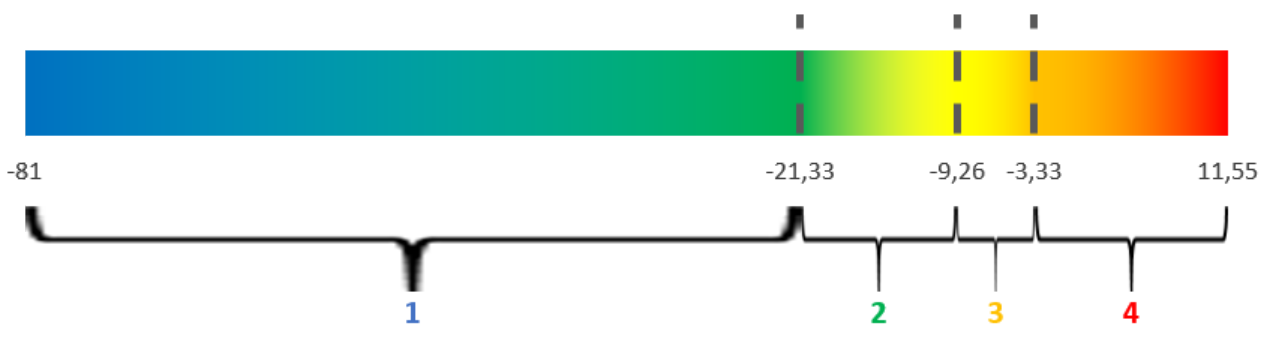
\includegraphics[width=.95\textwidth]{images/Quartil_glob.png}
\caption{Verteilung des Energiespektrums aller Energieprofile der globulären Proteine, in vier Perzentile, mit Grenzen.}
\label{fig:quartiles_glob}
\end{figure}

%new Quantile for globular:
%-81.29
%-21.53
%-9.50
%-3.44
%11.76
\begin{figure}
\centering
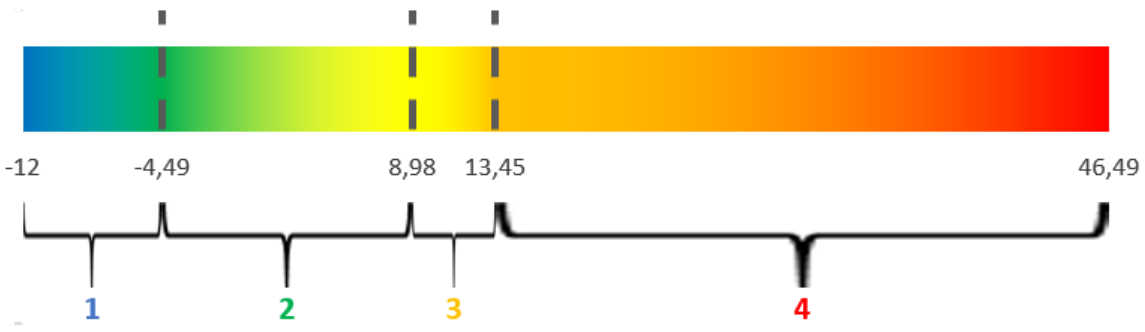
\includegraphics[width=.95\textwidth]{images/Quartil_memb.png}
\caption{Verteilung des Energiespektrums aller Energieprofile der Membran assoziierten Proteine, in vier Perzentile, mit Grenzen.}
\label{fig:quartiles_memb}
\end{figure}

%Quantile for membrane:
%-12.23
%4.49
%8.98
%13.45
%46.49

Ein dargestelltes Perzentil erfasst genau 25\% aller Energiewerte, man spricht deshalb auch von Quartilen. In \ac{Abb} \ref{fig:quartiles_glob} werden diese für alle globulären Proteine dargestellt. Das erste Quartil ist auch jenes mit dem größtem Spektrum, es reicht von -81 bis -22,21. Das zweite Quartil reicht von -21,33 bis -9,26. Das kleinste Quartil ist das dritte, es reicht von -9,26 bis -3,33 und das vierte Quartil reicht von -3,33 bis 11,55. 

In \ac{Abb} \ref{fig:quartiles_memb} werden die Quartile aller alpha helicalen Membran Proteine dargestellt, hier ist die relative Quartil Verteilung abweichend. Sodass die obere und untere Grenze sich deutlich von \ac{Abb} \ref{fig:quartiles_glob} unterscheiden, denn die untere Grenze beginnt bei -12 anstelle von -81. Die obere Grenze hingegen reicht bis +46,49 anstelle von +11,5. Demnach ist das erste Quartil von -12 bis -4,49 nicht mehr jenes mit dem größten Spektrum. Das zweite Quartil reicht von -4,49 bis 13,45, gefolgt vom drittem Quartil mit 8,98 bis 13,45.

Aufgrund der Übersichtlichkeit und durch die geringe Anzahl an alpha helicalen \ac{EP}s, befasst sich diese Arbeit hauptsächlich mit globulären Proteinen. 


\subsection{Spektrum aller Aminosäuren}

Die visualisierten Spektren der jeweiligen Aminosäuren zeigen deutliche Unterschiede auf, wie in \ac{Abb} \ref{fig:energy_ranges} zu sehen ist.

\begin{figure}
    \centering
    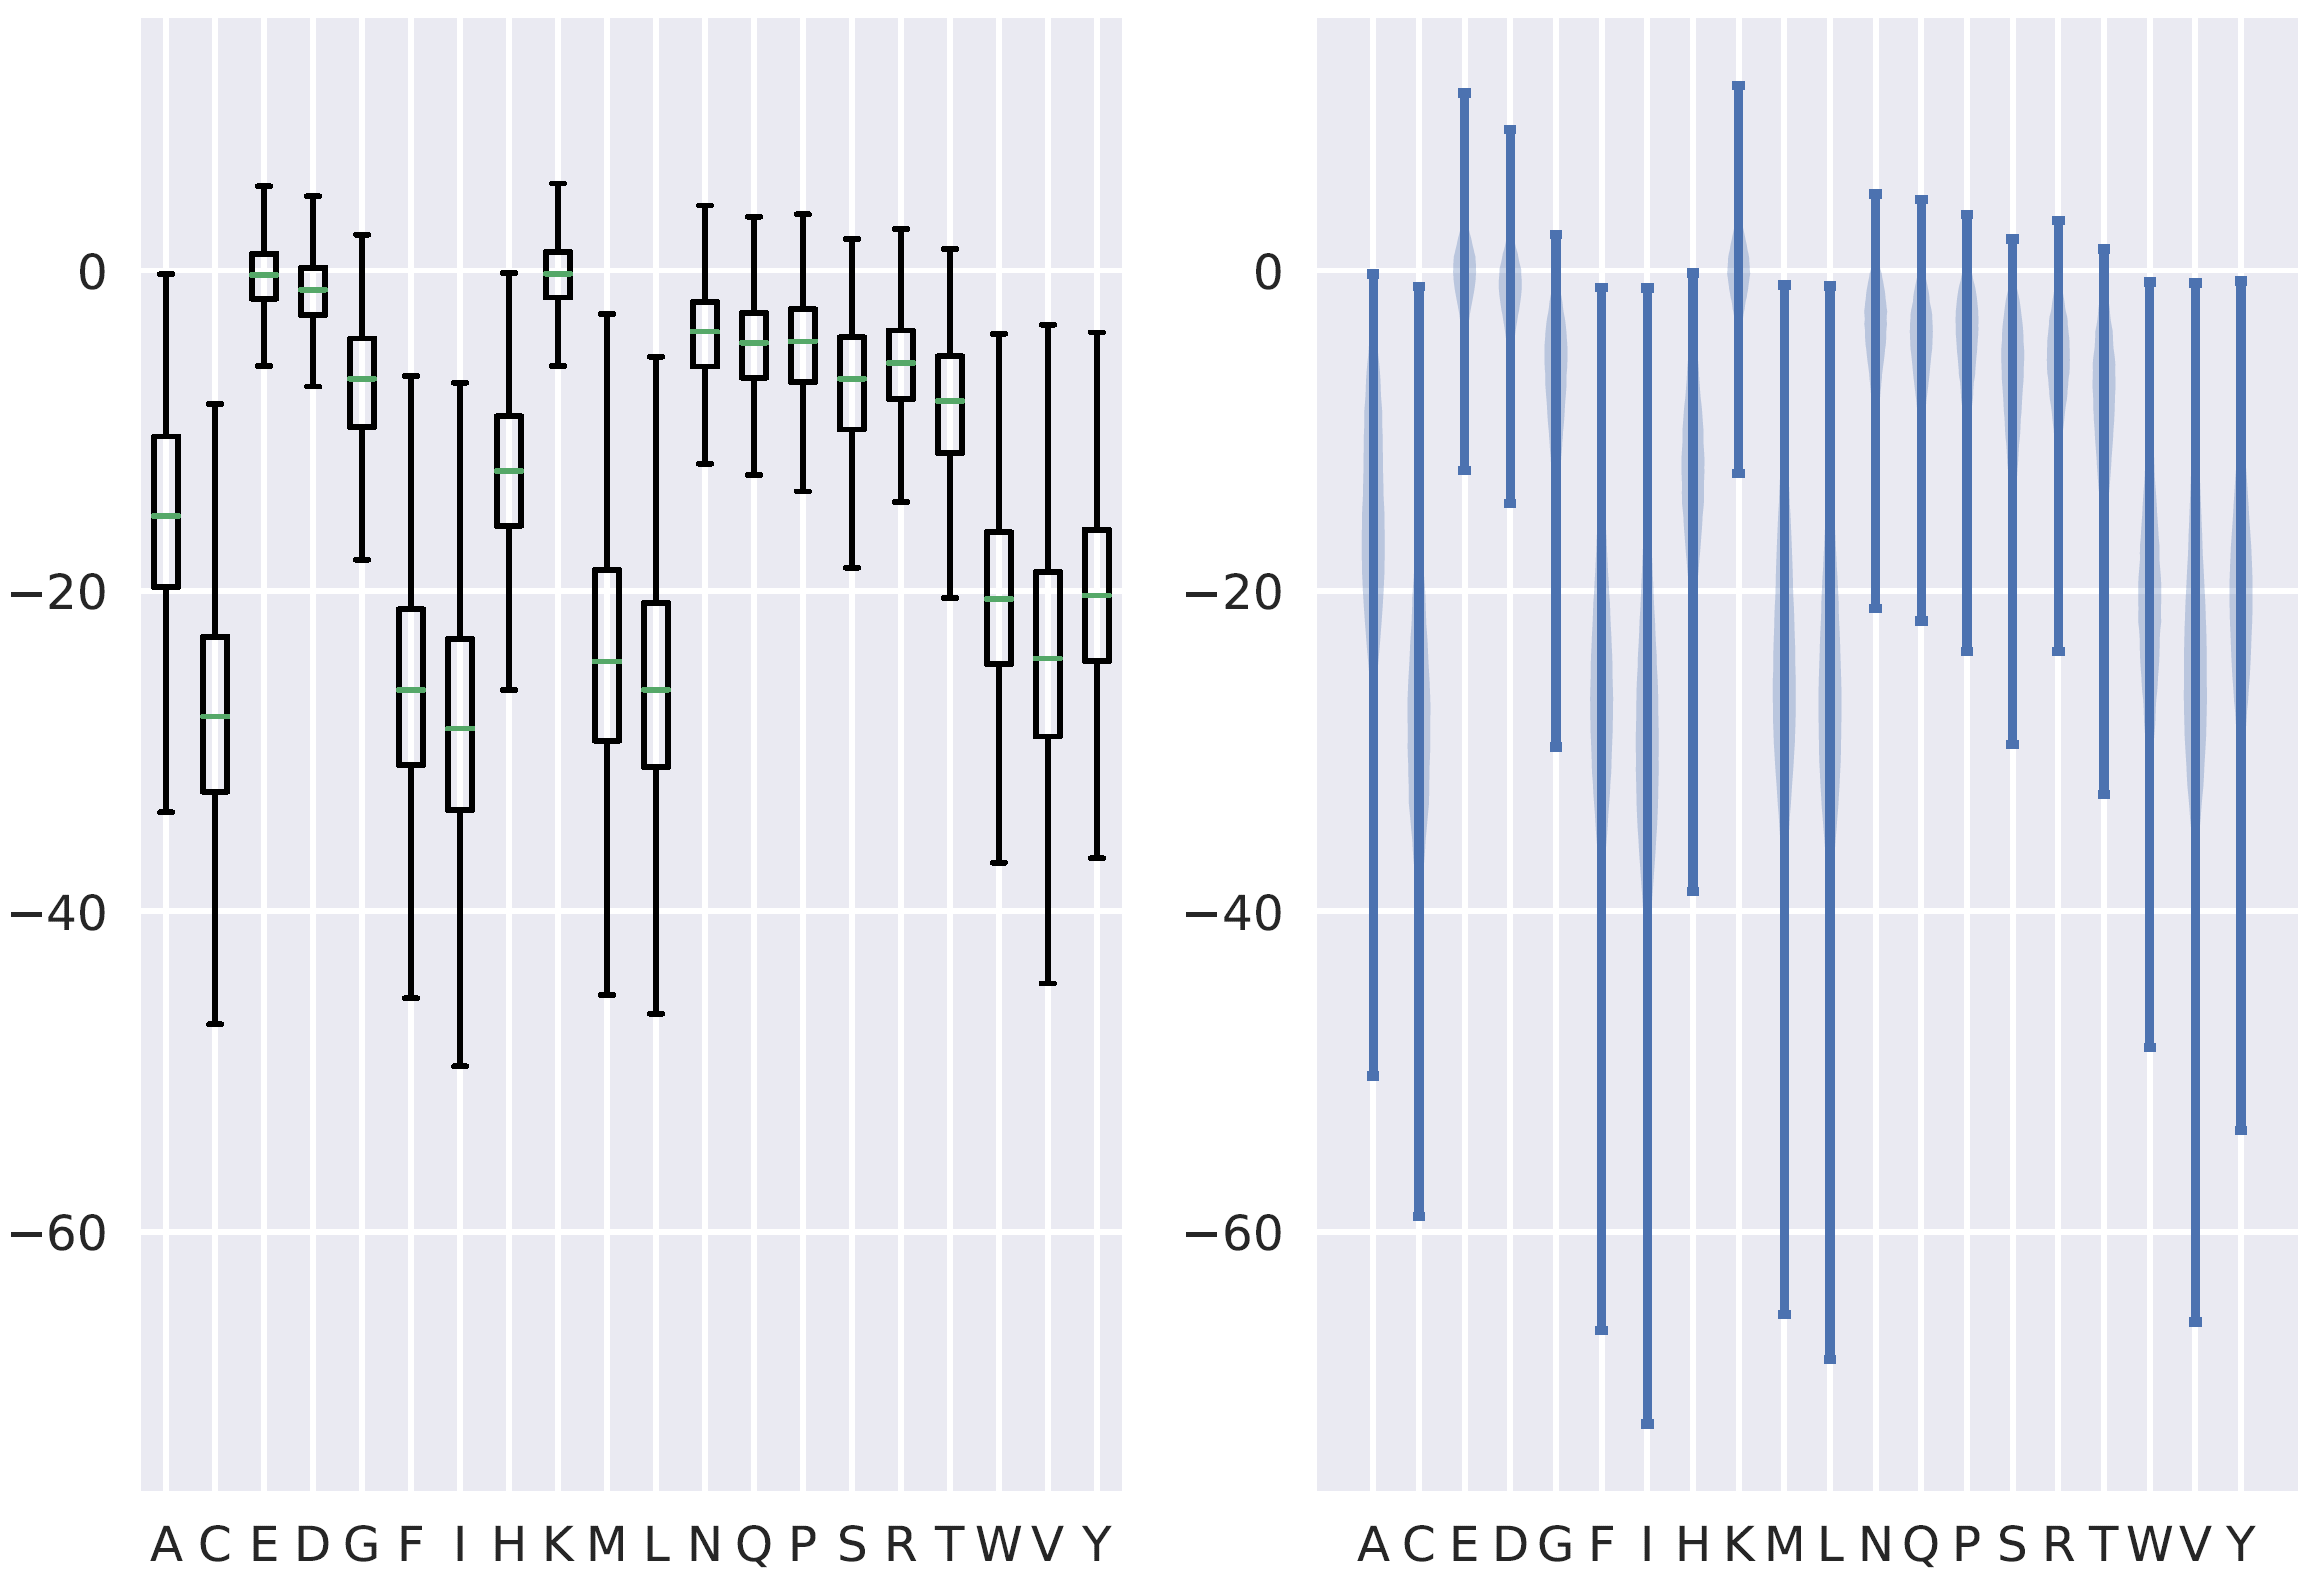
\includegraphics[width=.99\textwidth]{images/BoxPlot_energy_rages.png}
    \caption{Energien pro Aminosäure im Boxplot links und Violin Plot rechts dargestellt. Auf der Abszisse stellen die Buchstaben Abkürzungen der einzelnen Aminosäuren dar, siehe Tabelle \ref{tab:amino_table}. Auf der Ordinate sind die Energiewerte aufgetragen. Bei dem Boxplot wurden die Ausreißer mittels Grubbs-Test entfernt und die Mittelwerte mit einer grünen Markierung eingezeichnet.}
    \label{fig:energy_ranges}
\end{figure}

Zum Beispiel reicht das Spektrum der \ac{APs} von Glutaminsäure und Asparaginsäure von etwa -6 bis +6, während sich das Spektrum von Phenylalanin und Isoleuchin von -50 bis -6 bewegt. 

Zusätzlich zum Boxplot ist noch ein Violinen Plot für jede Aminosäure zu sehen. Dieser zeigt nochmals die Verteilung der Energiewerte innerhalb einer Aminosäure. Es ist so deutlich zu sehen, dass alle Werte um einen Mittelwert verteilt sind, sowie dass die Anzahl der Werte stark abflacht, sobald man sich den äußeren Bereich des jeweiligen Spektrums nähert.

Der Violinen Plot beinhaltet zudem noch alle Ausreißer, aufgrund dessen sich das Spektrum im allgemeinen länger darstellt, als es im Boxplot der Fall ist. Die Ausreißer wurden im Boxplot, mit Hilfe des Grubbs-Test \cite{Jain.2010}, herausgefiltert. 


\newpage
\subsection{Spektrum der Aminosäuren im Detail}
In diesem Abschnitt wird das Spektrum der zwei Aminosäuren, Glutaminsäure und Glycin im Detail vorgestellt. Diese beiden Aminosäuren wurden exemplarisch ausgewählt, da sich alle Aminosäurespektren ähnlich verhalten. So ist in \ac{Abb} \ref{fig:ep_as_distr} deutlich zu sehen, dass alle Energiewerte der Glutaminsäure um einen Mittelwert (-0.1) verteilt sind. Dies verhält sich sehr ähnlich für Glycin, hier sind ebenfalls alle Werte um den Mittelwert (-5.1) verteilt. Jedoch fällt auf, dass die Kurve nicht ganz symmetrisch ist, wie in der Verteilung von Energiewerten der Glutaminsäure, sondern nach links flacher abfällt. 

\begin{figure}[H]
    \subfigure[\ac{AP} Verteilung von Glutaminsäure]{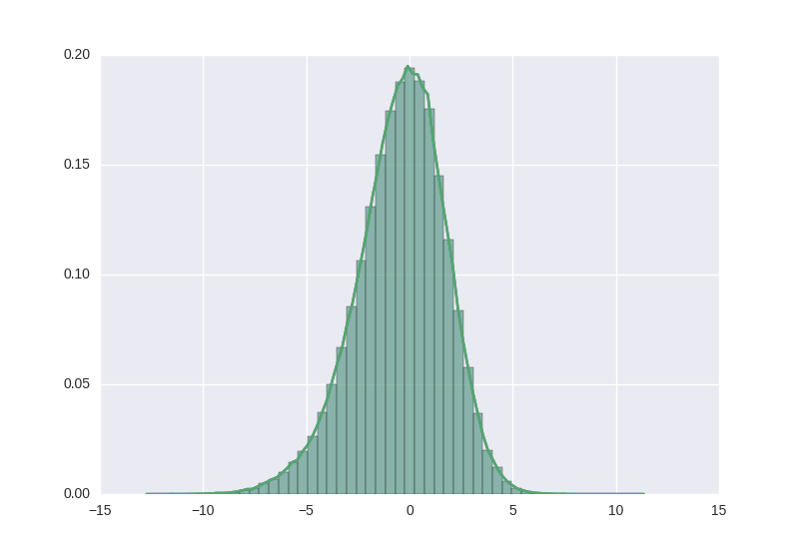
\includegraphics[width=0.49\textwidth]{images/Glutaminsaure_distr.png}}
    \subfigure[\ac{AP} Verteilung von Glycin]{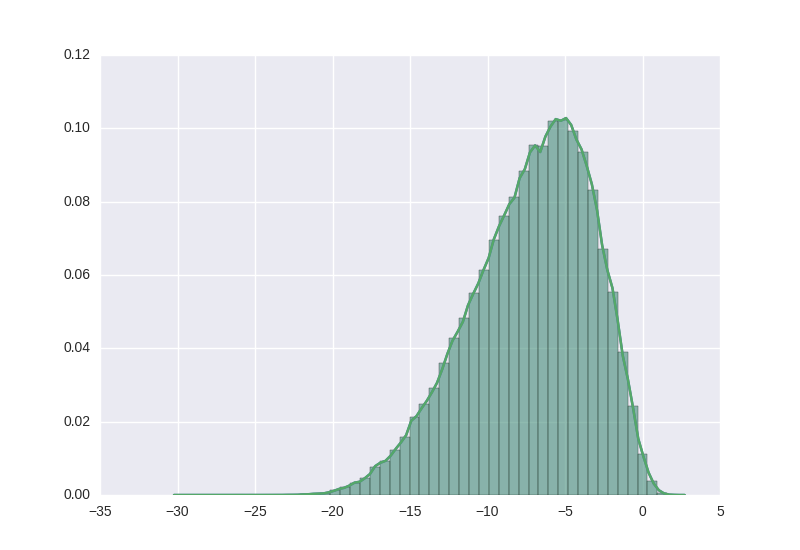
\includegraphics[width=0.49\textwidth]{images/histogramm_G.png}}
    \caption{Distribution der Energiewerte von Glutaminsäure links und Glycin rechts. Auf der Abszisse sind die Energiewerte aufgetragen und auf der Ordinate ihr relatives Vorkommen als Dezimalzahl.} 
    \label{fig:ep_as_distr}
\end{figure}

Ein Test auf Normalverteilung  hat ergeben, dass die Energiewerte nicht normalverteilt sind, da die Kurve eine zu geringe Varianz aufweist. 

Weil auch die restlichen Plots ähnlich aussehen, sind sie hier nicht dargestellt, sondern im Online Anhang dieser Arbeit zu finden.



\section{Ausgewählte Gene und SNPs}
Die in Kapitel \ref{sec:clinvar_filter} ausgesuchten \ac{SNP}s sind nun hier in Tabelle \ref{tab:expert_snps} und \ref{tab:multiple_subs_snps} dargestellt:

\begin{table}[H]
    \centering
    \caption{Tabelle aller Gene des \emph{expert panels} mit mindestens 10 pathogenen \ac{SNP}s. Die verwendeten Gene sind grün markiert.}
    \label{tab:expert_snps}
    \resizebox{\linewidth}{!}{%
    \begin{tabular}{llllllll}
    \hline
    \multicolumn{1}{|l|}{Name} & \multicolumn{1}{l|}{Template} & \multicolumn{1}{l|}{Länge} & \multicolumn{1}{l|}{Coverage} & \multicolumn{1}{l|}{Identität} & \multicolumn{1}{l|}{QMEAN} & \multicolumn{1}{l|}{SNPs} & \multicolumn{1}{l|}{Assoziierung} \\ \hline
    \rowcolor[HTML]{9AFF99} 
    MSH2 & 3thw.1.A & 934 & 98,40\% & 100\% & -2,05 & 33 & globulär \\ \hline
    \multicolumn{1}{|l}{BRCA1} & 1jm7.1.A & 1863 & 5,50\% & 100\% & -0,13 & 24 & \multicolumn{1}{l|}{globulär} \\
    \multicolumn{1}{|l}{} & 4y18.1.A &  & 11,40\% &  & -2,18 &  & \multicolumn{1}{l|}{} \\ \hline
    BRCA2 & 1miu.1.B & 3418 & 21\% & 75,48\% & -5,05 & 10 & globulär \\
    \rowcolor[HTML]{9AFF99} 
    CFTR & 5uak.1.A & 1480 & 96,70\% & 100\% & -4,51 & 44 & membran \\
    MYH7 & 5tby.1.A & 1935 & 49,50\% & 100\% & -4,8 & 32 & globulär \\ \hline
    \multicolumn{1}{|l}{MLH1} & 4p7a.1.A & 756 & 44\% & 100\% & -0,73 & 65 & \multicolumn{1}{l|}{globulär} \\
    \multicolumn{1}{|l}{} & 3rbn.1.A &  & 34,90\% & 100\% & -1,29 &  & \multicolumn{1}{l|}{} \\ \hline
    \end{tabular}}
\end{table}

Wie in der ersten Tabelle zu sehen ist, ist die größte Coverage bei \texttt{MSH2} mit 98,4\%, gefolgt von \texttt{CFTR} mit 96,7\%. Die Sequenzidentität beträgt bei beiden 100\%. Bei fast allen Sequenzen wurden mehrere Templates gefunden, doch die Meisten weisen eine sehr niedrige Coverage auf, sodass sie hier nicht dargestellt sind. Bei \texttt{MLH1} wurden zwei Templates gefunden, welche 44\% und 34,9\% der Sequenz abdecken. Bei \texttt{BRCA1} wurden ebenfalls mehrere Templates gefunden, sodass hier eine Coverage von 11,4\% und 5,5\% vorliegt. \texttt{BRCA2} hat eine Coverage von 21\% bei 75,48\% Sequenzidentität. Letztendlich wurden nur die \ac{SNP}s von \texttt{MSH2} und \texttt{CFTR} in dieser Arbeit verwendet.

In einem zweiten Durchgang wurden auch alle Proteine mit ihren SNPs aus Tabelle \ref{tab:multiple_subs_snps} mittels Swissmodel strukturell modelliert. Hierbei zeigte \texttt{ABCA4} die höchste Coverage mit 98,90\% und Sequenzidentität von 51,97\%. Betrachtet man Coverage und Sequenzidentität in Abhängigkeit, so weist \texttt{ACADM} die höchste Coverage mit 91,7\% und \texttt{SLC2A1} die zweit höchste mit 90,7\% auf. Die Sequenzidentität beträgt bei \texttt{ACADM} 100\% und bei \texttt{SLC2A1} 99,59\%, dies bedeutet, dass bei \texttt{SLC2A1}, im Vergleich zur Swissmodel Referenz, alle bis auf eine Aminosäure übereinstimmen.

Zusätzlich wurden noch \texttt{KCNQ1}, \texttt{KCNH2} und \texttt{SDHB} in den Datnesatz aufgenommen. Die restlichen Gene wurden nicht in den Datensatz aufgenommen.

\begin{table}[]
    \centering
    \caption{Tabelle aller Gene der ClinVar Datenbank, mit mindestens 6 pathogenen SNPs und multiplen Autoren, ohne Widerspruch. Dunkles grün steht für eine gute Coverage und Sequenzidentität, hellgrün zeigt die Gene, welche keine so hohe Coverage aufweisen, aber dennoch in den Datensatz aufgenommen wurden.}
    \label{tab:multiple_subs_snps}
    \resizebox{\linewidth}{!}{%
    \begin{tabular}{llllllll}
    \hline
    \multicolumn{1}{|l|}{Name} & \multicolumn{1}{l|}{Template} & \multicolumn{1}{l|}{Länge} & \multicolumn{1}{l|}{Coverage} & \multicolumn{1}{l|}{Identität} & \multicolumn{1}{l|}{QMEAN} & \multicolumn{1}{l|}{SNPs} & \multicolumn{1}{l|}{Assoziierung} \\ \hline
    MFN2 & 5gom.1.A & 757 & 51,30\% & 71.21\% & -1,32 & 13 & globulär \\
    \rowcolor[HTML]{CBFFCB} 
    SDHB & 1zoy.1.B & 280 & 85,70\% & 97.54\% & -0,88 & 10 & Membran \\
    MUTYH & 3n5n.2.A & 535 & 51,40\% & 100\% & -1,8 & 14 & globulär \\
    ALPL & 1zef.1.A & 524 & 90\% & 58,58\% & -2,04 & 8 & globulär \\
    \rowcolor[HTML]{9AFF99} 
    SLC2A1 & 4pyp.1.A & 492 & 90,70\% & 99,59\% & -4,75 & 8 & Membran \\
    \rowcolor[HTML]{9AFF99} 
    ACADM & 1ege.1.B & 421 & 91,70\% & 100\% & -1,23 & 11 & globulär \\
    LMNA & 1ufg.1.A & 572 & 22,70\% & 96,18\% & -4,66 & 21 & globulär \\
    ABCA4 & 5xjy.1.A & 2273 & 98,90\% & 51,97\% & -6,57 & 22 & Membran \\
    TNNT2 & 1j1d.2.B & 295 & 25,10\% & 99,03\% & 0,87 & 10 & globulär \\
    COL9A2 & 5ctd.1.B & 689 & 6,30\% & 86,67\% & 0,41 & 6 & globulär \\
    STIL & 4yyp.1.B & 1288 & 100\% & 2\% & -0,03 & 6 & globulär \\
    AGL & 5d06.2.A & 1532 & 43,09\% & 97,30\% & -4,43 & 8 & globulär \\
    \rowcolor[HTML]{CBFFCB} 
    KCNQ1 & 5vms.1.A & 676 & 68,50\% & 83,30\% & -5,87 & 10 & Membran \\
    \rowcolor[HTML]{CBFFCB} 
    KCNH2 & 5va2.1.A & 1159 & 74,20\% & 96,56\% & -5,38 & 6 & Membran \\
    PMS2 & 1h7s.1.A & 862 & 39\% & 100\% & 0,25 & 6 & globulär
    \end{tabular}}
\end{table}



\section{SNPs in Energieprofilen}

Die in Kapitel \ref{sec:plot_eps} berechneten Plots sind nun hier dargestellt, in \ac{Abb} \ref{fig:comp_plot_MSH2} ist ein beispielhafter Ausschnitt aus dem globulären Protein \texttt{MSH2} dargestellt. Die Abszisse gibt die Positionen der fortlaufenden Aminosäuren an, auf der Ordinate befinden sich die Energiewerte. Zu sehen ist im oberen Bild die Referenzsequenz in Blau und die Sequenz mit dem \ac{SNP} Ile169Val in Rot. Die mutierte Sequenz ist nur sichtbar, wenn sie sich von der Referenzsequenz unterscheidet, zum besseren Überblick ist zusätzlich noch die Differenz der beiden Sequenzen als die grüne Linie aufgetragen. Die gelbe Markierung zeigt die Position der \ac{SNP}s. 

\begin{figure}
    \centering
    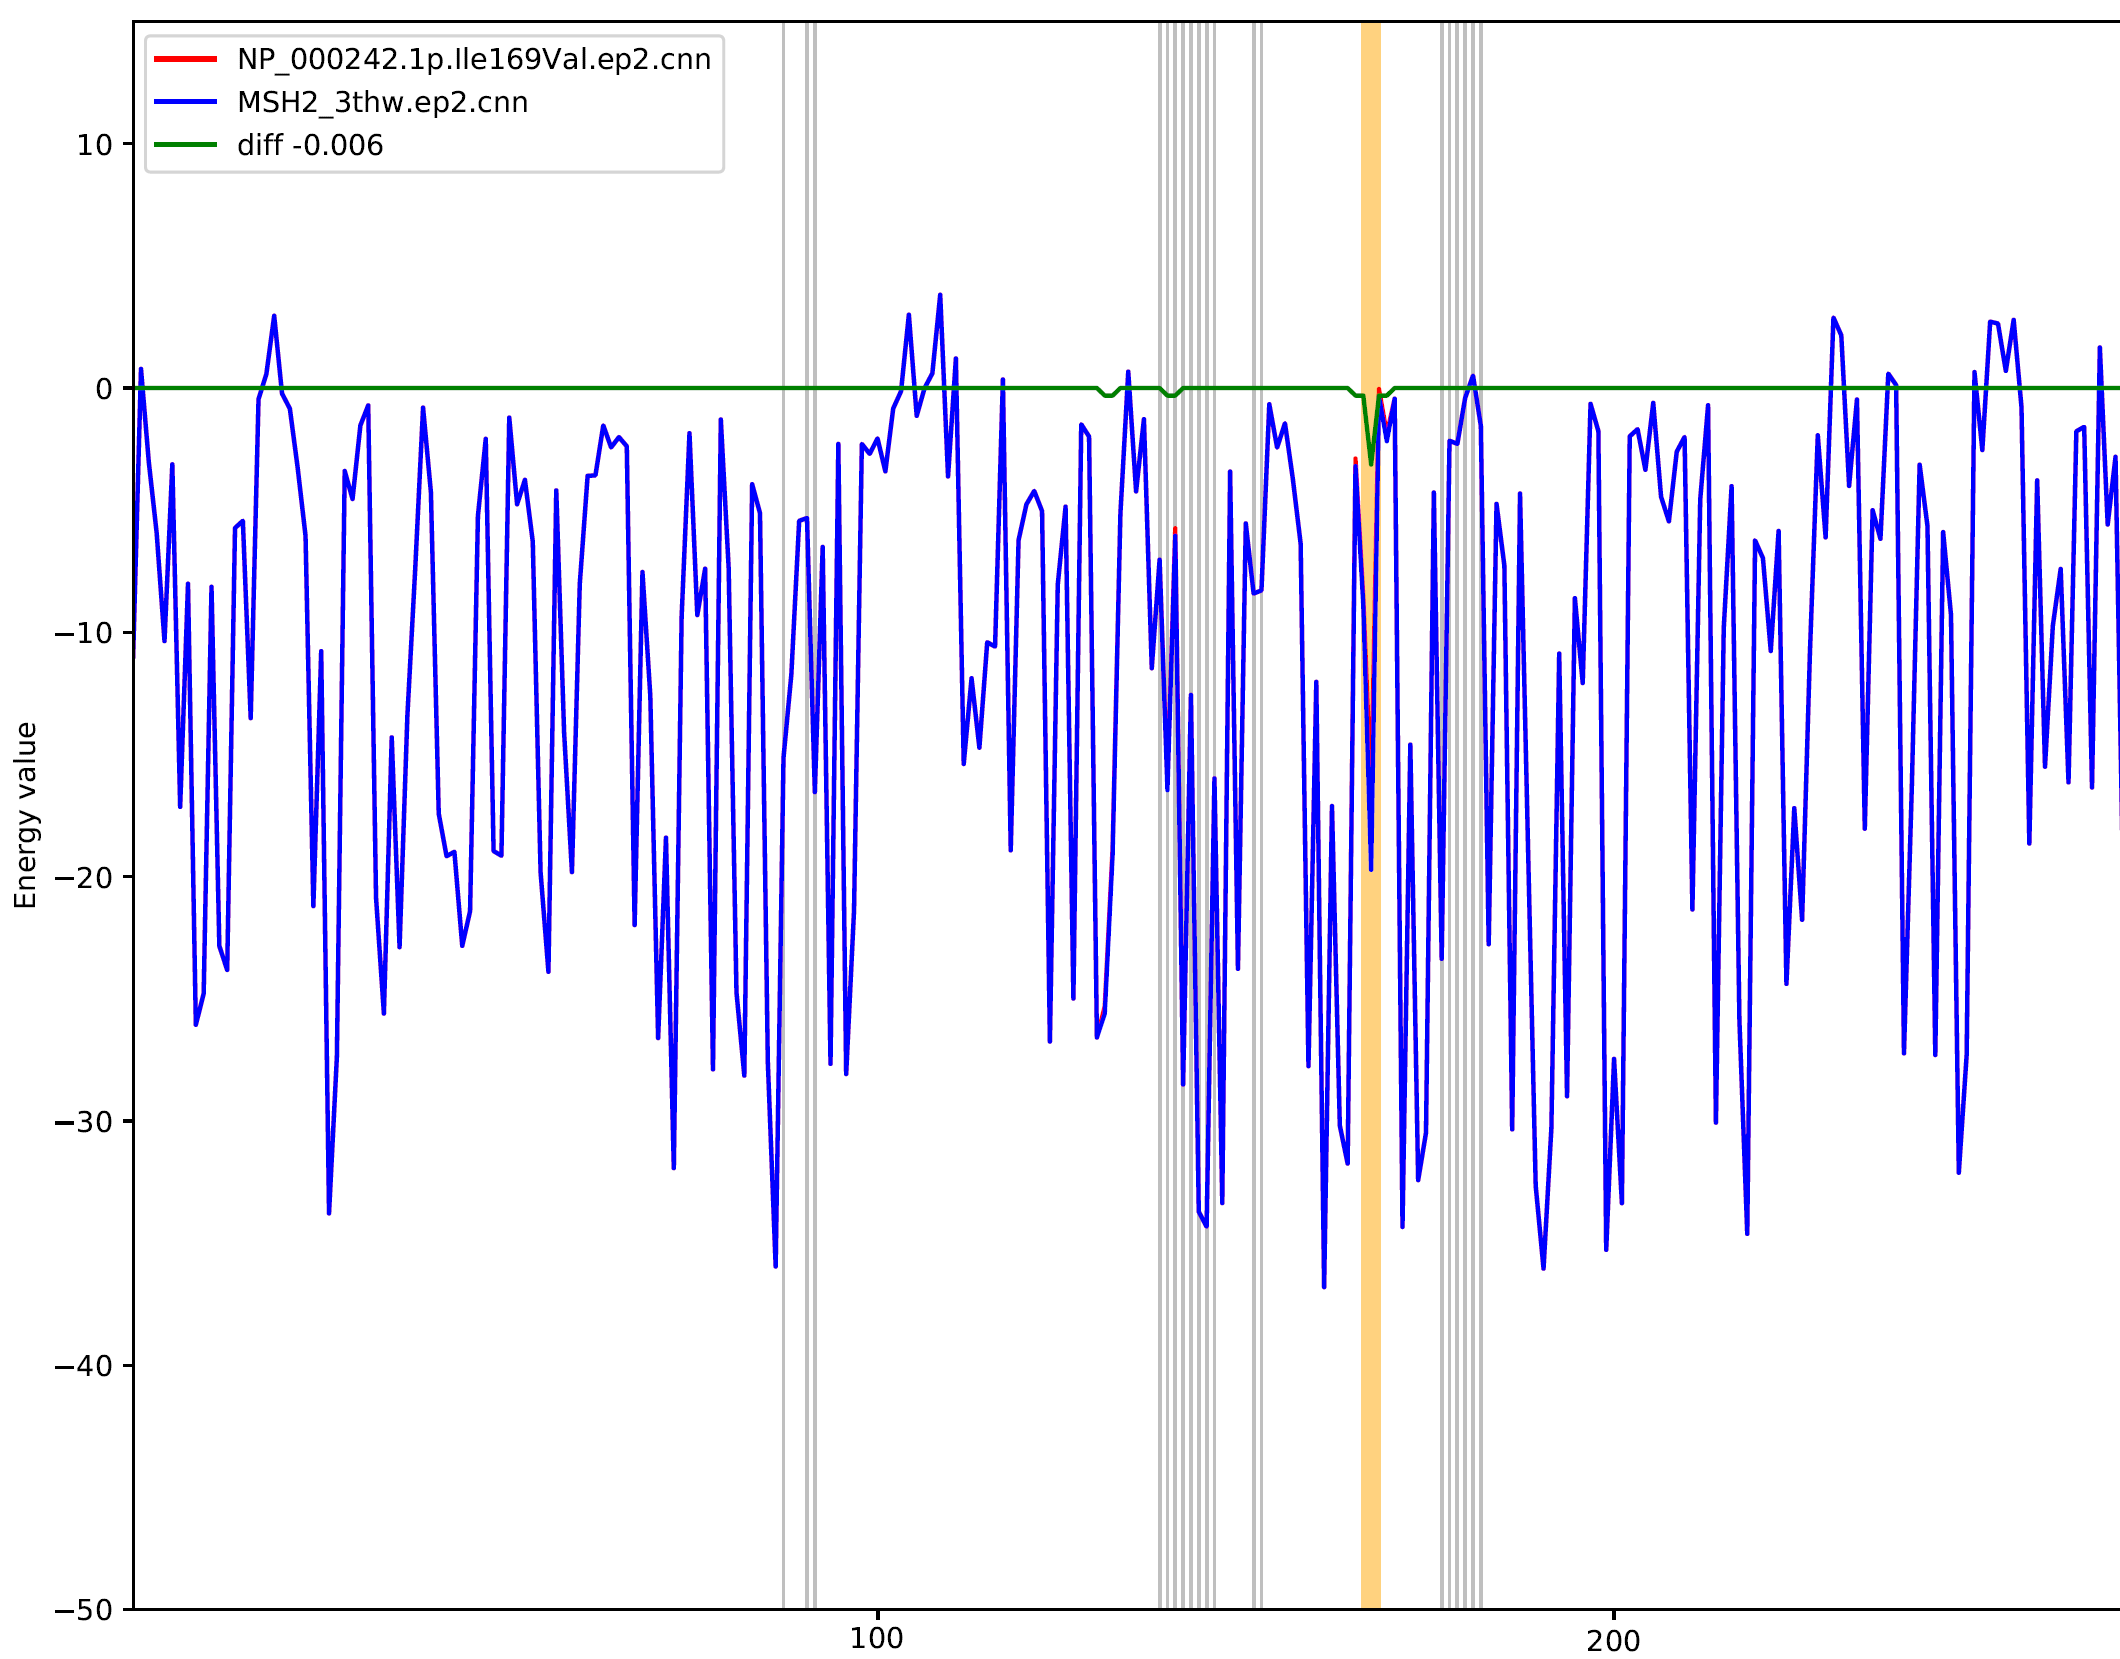
\includegraphics[width=.90\textwidth]{images/comp_plot_Ile169Val.png}
    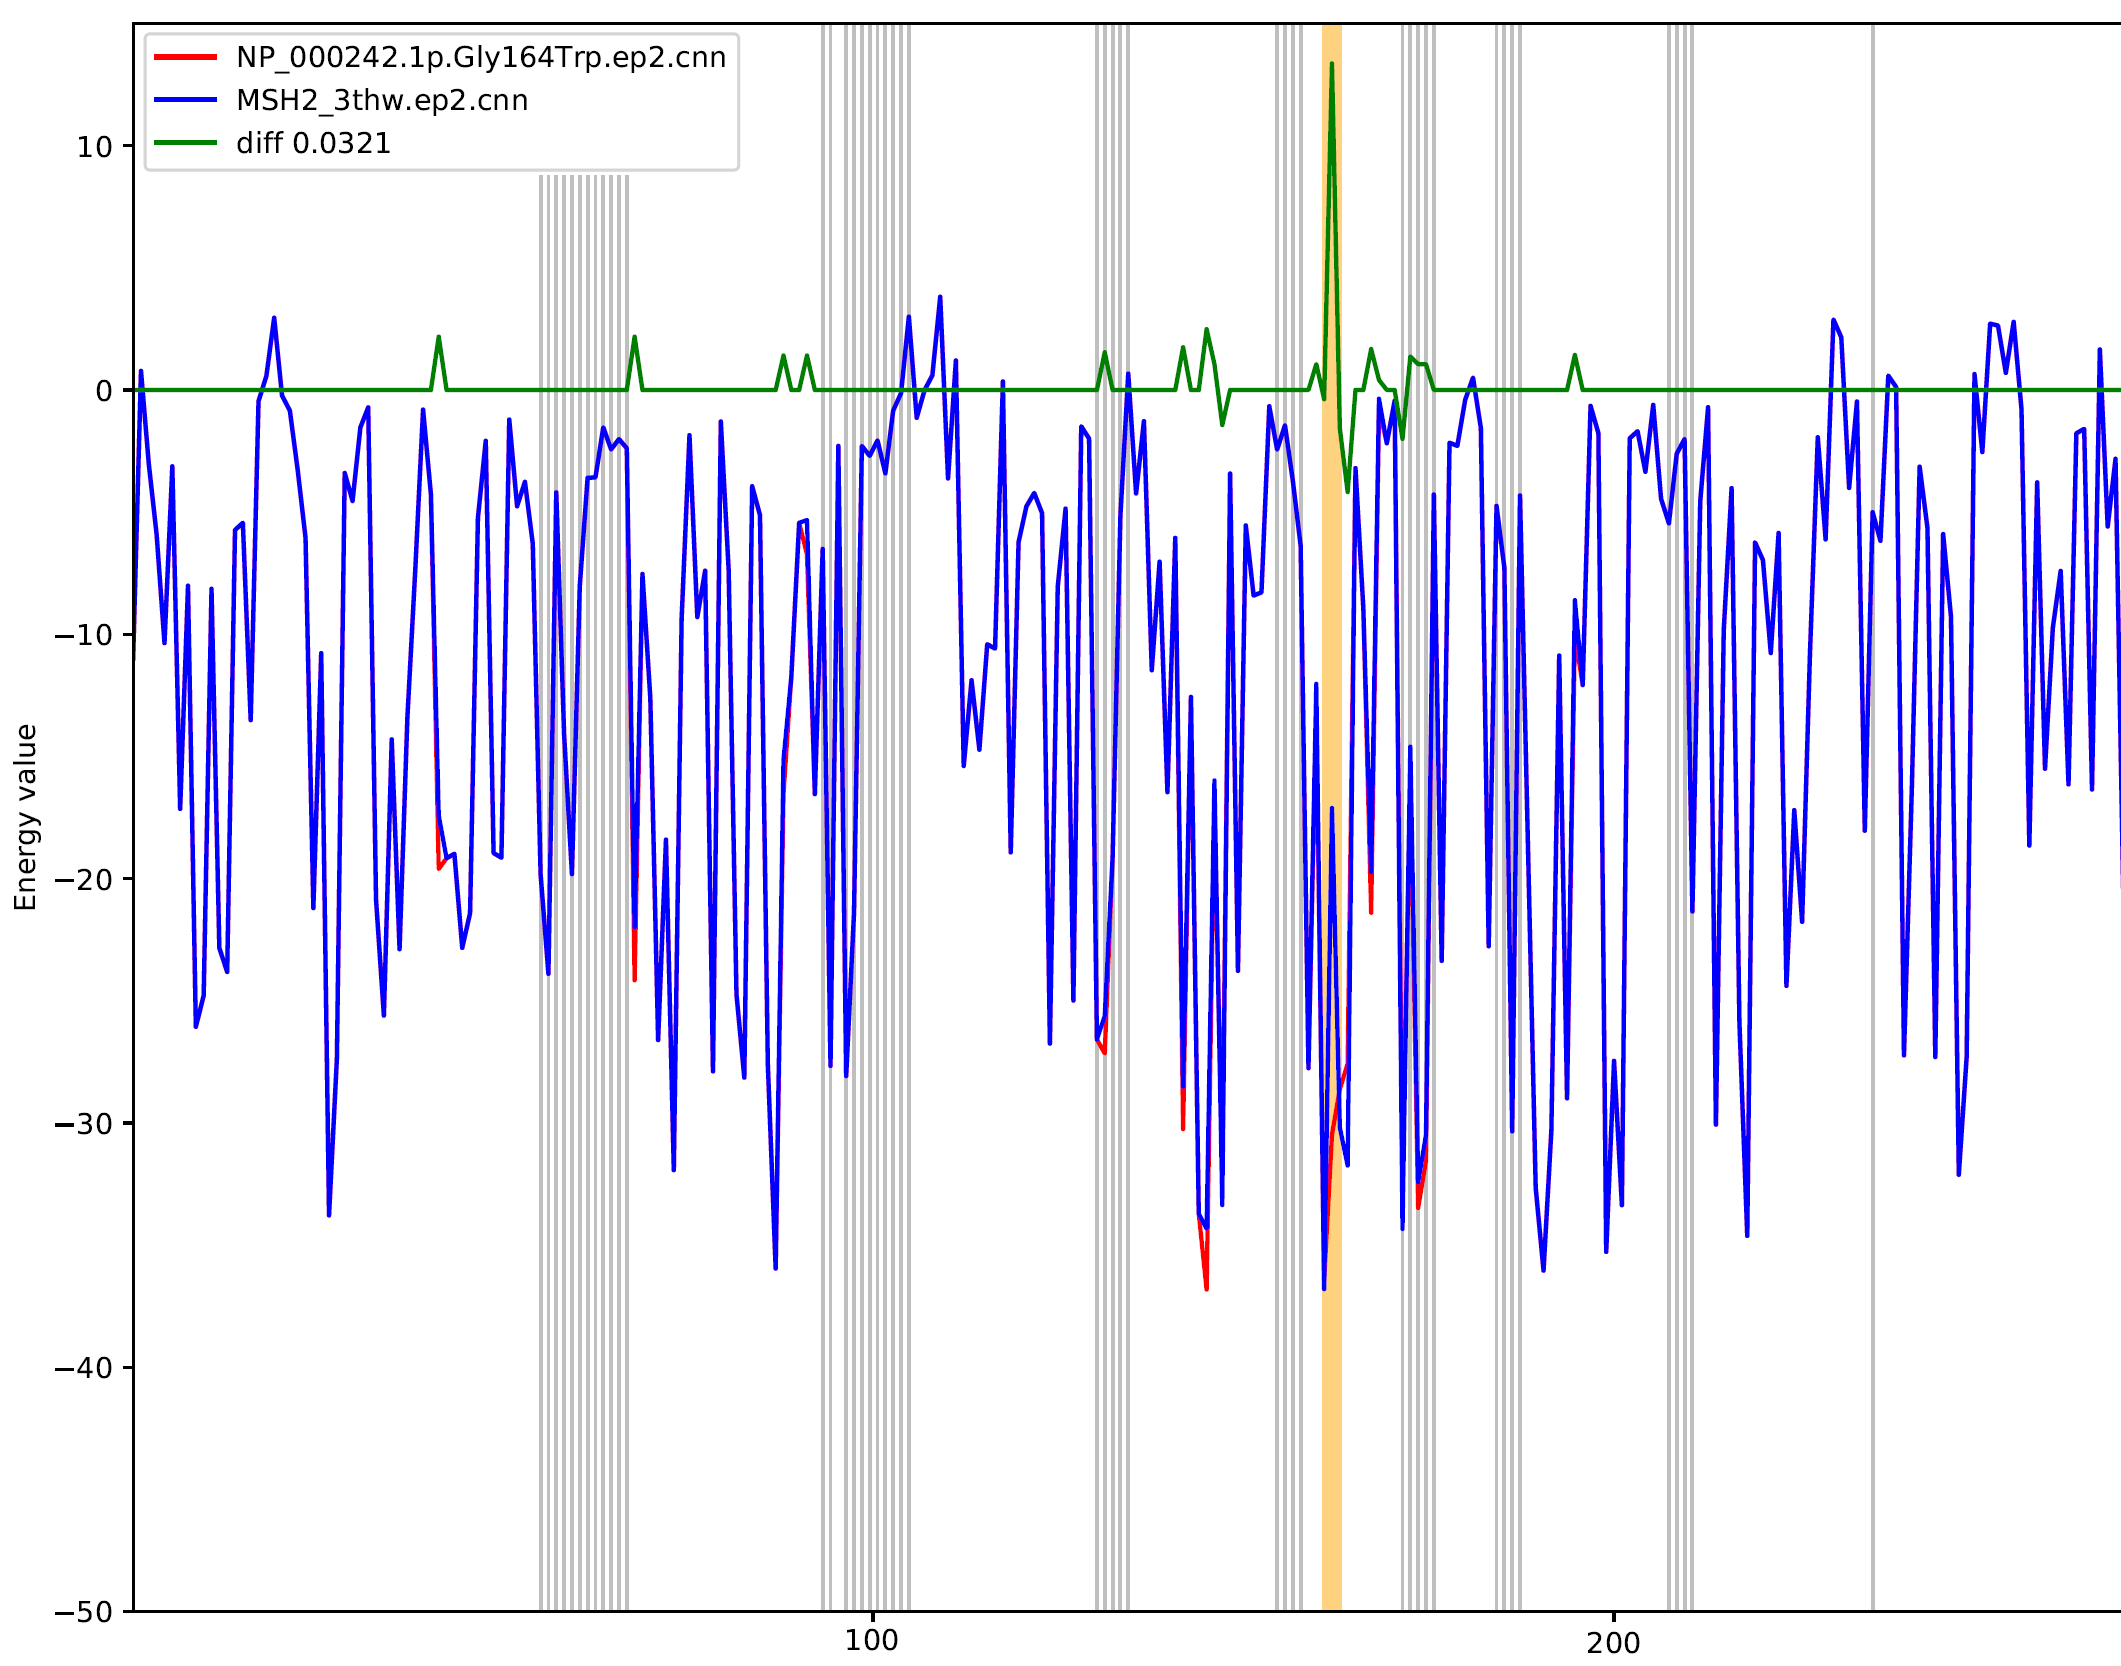
\includegraphics[width=.90\textwidth]{images/comp_plot_Gly164Trp.png}
    \caption{Ausschnitt aus dem Protein MSH2 mit gutartigem \ac{SNP} an Position 169 und mit pathogenen \ac{SNP} an Position 164. Auf der Abszisse ist die Aminosäureposition und auf der Ordinate sind die Energiewerte aufgetragen. Die Referenzsequenz ist blau, die mutierte Sequenz rot und die Differenz der beiden Sequenzen grün dargestellt. Die Position des \ac{SNP}s ist gelb markiert. Die gesamte Energiedifferenz über alle Aminosäuren ist in der Legende hinter \emph{diff} angegeben.} 
    \label{fig:comp_plot_MSH2}
\end{figure}

So ist an der Position des \ac{SNP}s, sowohl im oberen als auch im unterem Bild eine Veränderung des Energieniveaus zu erkennen. Im oberen Bild wurde ein gutartiger \ac{SNP} geplottet, zu sehen ist eine Substitution von Isoleucin nach Valin an Position 169, das Energieniveau verändert sich um 2,5 Einheiten. 

Im unteren Bild wurde ein pathogener \ac{SNP} geplottet, zu sehen ist hier eine Substitution von Glycin nach Tryptophan an Position 164, das Energieniveau verändert sich um 12,8 Einheiten. 

Zudem wurden nicht nur Veränderungen unmittelbar am \ac{SNP} festgestellt, sondern auch einige nicht ganz so starke Veränderungen an verschiedenen anderen Aminosäuren im Protein, diese Veränderungen treten oft an den vorher berechneten Kontakten der Aminosäure auf. Generell lässt sich sagen, dass es im gesamten Protein zu energetischen Veränderungen kam.

\begin{figure}
    \centering
    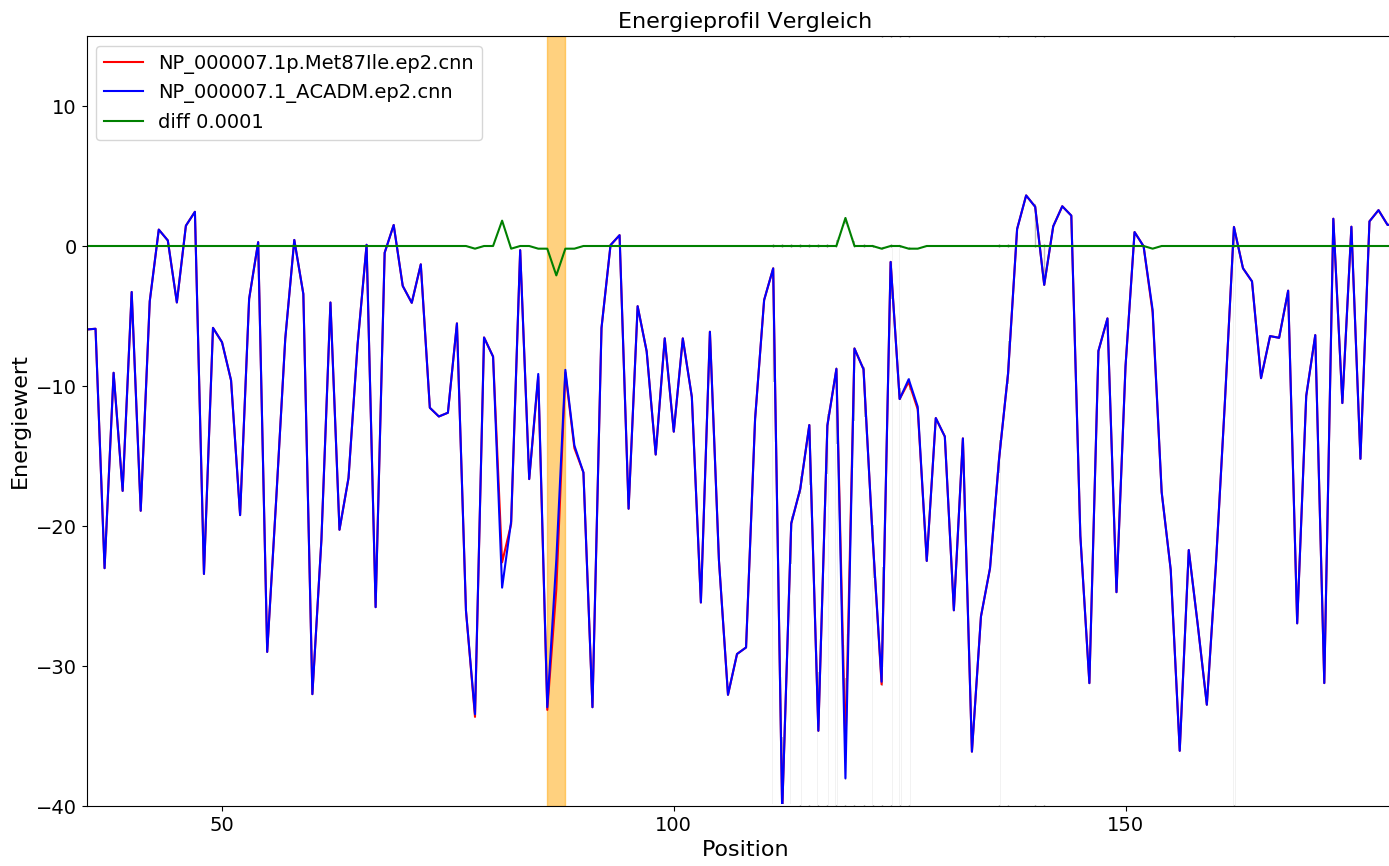
\includegraphics[width=.95\textwidth]{images/comp_plot_ACADM_Met87Ile.png}
    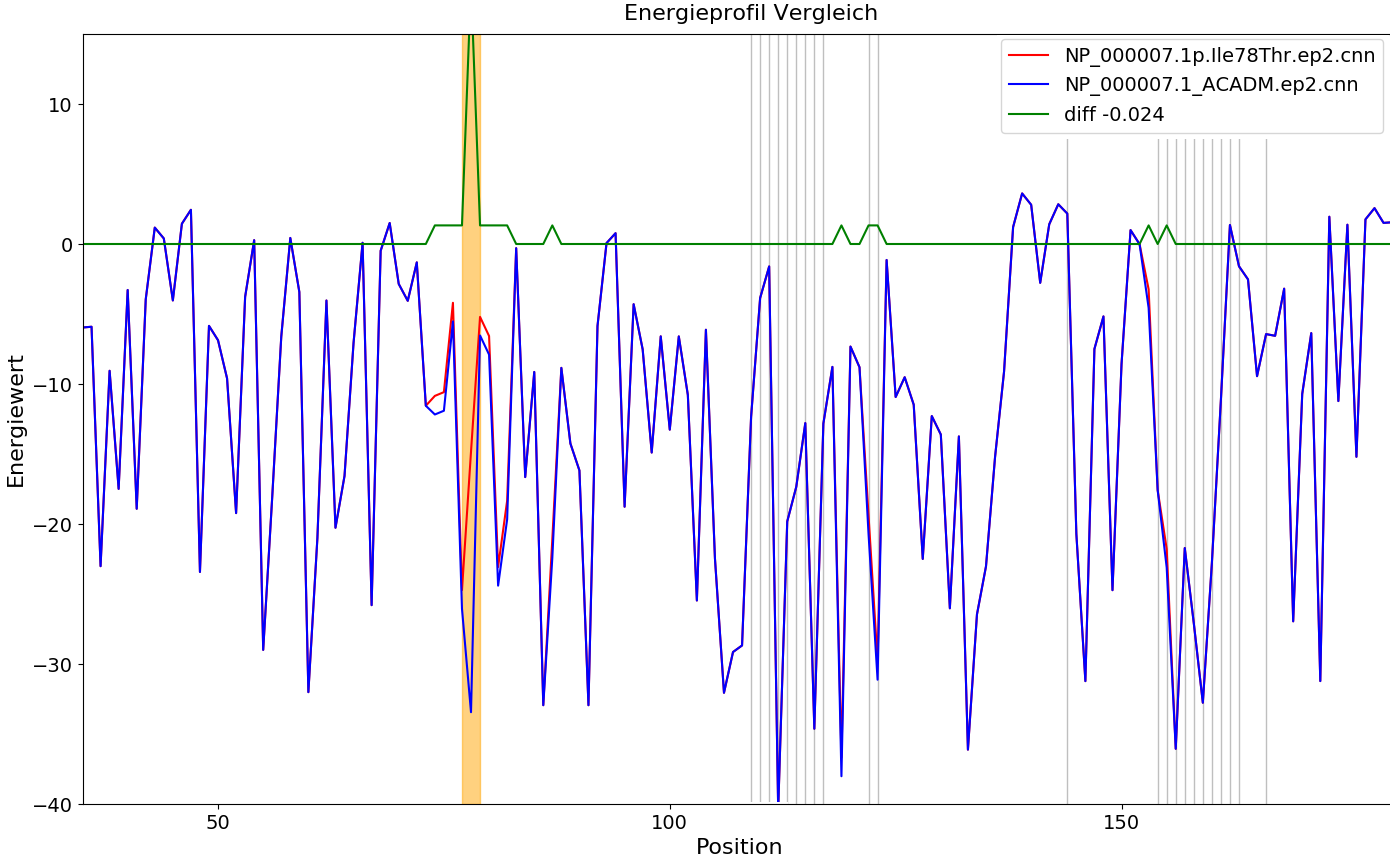
\includegraphics[width=.95\textwidth]{images/comp_plot_ACADM_Ile78Thr.png}
    \caption{Ausschnitt aus dem Protein ACADM mit gutartigem \ac{SNP} an Position 78 und mit pathogenen \ac{SNP} an Position 87. Auf der Abszisse ist die Aminosäureposition und auf der Ordinate sind die Energiewerte aufgetragen. Die Referenzsequenz ist blau, die mutierte Sequenz rot und die Differenz der beiden Sequenzen grün dargestellt. Die Position des \ac{SNP}s ist gelb markiert. Die gesamte Energiedifferenz über alle Aminosäuren ist in der Legende hinter \emph{diff} angegeben.}
    \label{fig:comp_plot_ACADM}
\end{figure}

Als weiteres Beispiel dient die \ac{Abb} \ref{fig:comp_plot_ACADM}, hier ist der Anfang des globulären Proteins \texttt{ACADM} dargestellt. Diese Abbildung ist genau wie \ac{Abb} \ref{fig:comp_plot_MSH2} aufgebaut, so sind die fortlaufenden Aminosäuren auf der Abszisse und die Energiewerte befinden sich auf der Ordinate. Im oberen Bild der \ac{Abb} \ref{fig:comp_plot_ACADM} ist der \ac{SNP} Met87Ile eingetragen, der eine Substitution von Methionin nach Isoleucin an der Position 87 im Protein zeigt. Dies verringert den Energiewert an dieser Stelle um etwa 1,5, an den Kontakten und generell in der gesamtem Sequenz, wurden nur sehr kleine Veränderungen festgestellt.

Im unteren Bild der \ac{Abb} \ref{fig:comp_plot_ACADM}, ist eine Substitution an Position 78 von Isoleucin auf Threonin zu erkennen. Der Energiewert an dieser Position wurde um etwa 15 erhöht. Zwei Positionen vor und hinter dem \ac{SNP} sieht man ebenfalls eine Erhöhung des Energieniveau um 1,5.

Die restlichen Plots, also jene welche für die Erstellung der Tabellen \ref{tab:snps_memb} und \ref{tab:snps_glob} notwendig waren, befinden sich im Online Anhang dieser Arbeit.



\newpage
\section{Auswertung}
\label{sec:snp_auswertung}
Der Datensatz aus Kapitel \ref{sec:auswertung_eps} enthielt 85 \ac{SNP}s, da jedoch nicht alle SNPs innerhalb der aufgeklärten Struktur lagen, bestand der Datensatz am Ende aus 55 \ac{SNP}s, aus den Genen \texttt{MSH2, CFTR, ACADM, PMS2, SLC2A1} und \texttt{SDHB}. Nun wurde nach Kriterien gesucht, um diese SNPs zu trennen. 

\begin{table}[H]
    \centering
    \caption{Dargestellt sind alle alpha helicalen Membranproteine mit \ac{SNP}s, die auf den aufgeklärten Strukturen liegen. Die \texttt{SNP} Zeile gibt an welche Aminosäure an welcher Position ausgetauscht wurde. Die \texttt{ClinVar} Zeile zeigt die offizielle ClinVar Annotation des jeweiligen \ac{SNP}s an. Die \texttt{snp\_diff} Zeile zeigt die Differenz zwischen Mutation und Referenz. Die \texttt{snp\_diff\_amount} Zeile gibt die absolute Differenz zwischen Mutation und Referenz. Die \texttt{total\_diff} Zeile zeigt die Totale Energiedifferenz über die gesamte Polypeptidkette. Die \texttt{total\_contact\_diff} Zeile gibt die Energiedifferenz über alle Kontakte an. Pathogene \ac{SNP}s sind rot und gutartige \ac{SNP}s sind grün markiert, die Tabelle ist aufsteigend nach der blauen Kopfzeile sortiert.}
    \label{tab:snps_memb}
    \resizebox{\linewidth}{!}{%
    \begin{tabular}{llllll}
    \hline
    \multicolumn{1}{|l|}{SNP} & \multicolumn{1}{l|}{ClinVar} & \multicolumn{1}{l|}{\cellcolor[HTML]{BBDAFF}snp\_diff} & \multicolumn{1}{l|}{snp\_diff\_amount} & \multicolumn{1}{l|}{total\_diff} & \multicolumn{1}{l|}{total\_contact\_diff} \\ \hline
    \rowcolor[HTML]{FFCCC9} 
    Cys192Arg & pathogenic & -28,58 & 28,58 & 63,35 & 48,27 \\
    \rowcolor[HTML]{FFCCC9} 
    Cys196Tyr & pathogenic & -13,57 & 13,57 & 37,29 & 26,18 \\
    \rowcolor[HTML]{FFCCC9} 
    Ile127Ser & pathogenic & -7,07 & 7,07 & 15,16 & 11,25 \\
    \rowcolor[HTML]{FFCCC9} 
    Val140Phe & pathogenic & -2,53 & 2,53 & 15,71 & 5,36 \\
    \rowcolor[HTML]{9AFF99} 
    Gly53Glu & benign & -2,43 & 2,43 & 7,27 & 4,86 \\
    \rowcolor[HTML]{9AFF99} 
    His57Arg & benign & -1,21 & 1,21 & 4,85 & 2,08 \\
    \rowcolor[HTML]{9AFF99} 
    Ser163Pro & benign & -0,90 & 0,90 & 46,12 & 7,72 \\
    \rowcolor[HTML]{FFCCC9} 
    Pro197Arg & pathogenic & -0,39 & 0,39 & 3,20 & 0,62 \\
    \rowcolor[HTML]{FFCCC9} 
    Arg46Gln & pathogenic & 1,06 & 1,06 & 4,53 & 2,01 \\
    \rowcolor[HTML]{FFCCC9} 
    Arg230His & pathogenic & 2,43 & 2,43 & 7,28 & 5,37 \\
    \rowcolor[HTML]{FFCCC9} 
    Arg242His & pathogenic & 3,54 & 3,54 & 14,10 & 7,39 \\
    \rowcolor[HTML]{FFCCC9} 
    Trp200Cys & pathogenic & 8,74 & 8,74 & 69,42 & 19,57 \\
    \rowcolor[HTML]{FFCCC9} 
    Arg242Cys & pathogenic & 20,53 & 20,53 & 41,07 & 33,17
    \end{tabular}}
\end{table}

% Please add the following required packages to your document preamble:
% \usepackage[table,xcdraw]{xcolor}
% If you use beamer only pass "xcolor=table" option, i.e. \documentclass[xcolor=table]{beamer}
\begin{table}[]
    \centering
    \caption{Zu sehen sind alle globulären Proteine, mit ihren jeweiligen \ac{SNP}s. Die Tabelle ist genau wie \ref{tab:snps_memb} aufgebaut, mit dem Zusatz, dass \ac{SNP}s welche widersprüchliche Annotationen haben grau und \ac{SNP}s mit nur einem Autor hell grün dargestellt sind.}
    \label{tab:snps_glob}
    \resizebox{\linewidth}{!}{%
    \begin{tabular}{llllll}
        \hline
        \multicolumn{1}{|l|}{SNP} & \multicolumn{1}{l|}{ClinVar} & \multicolumn{1}{l|}{snp\_diff} & \multicolumn{1}{l|}{\cellcolor[HTML]{BBDAFF}snp\_diff\_amount} & \multicolumn{1}{l|}{total\_diff} & \multicolumn{1}{l|}{total\_contact\_diff} \\ \hline
        \rowcolor[HTML]{FFCCC9} 
        Gly164Arg & pathogenic & -0,27 & 0,27 & 265,91 & 46,75 \\
        \rowcolor[HTML]{FFCCC9} 
        Leu84Phe & pathogenic & 0,78 & 0,78 & 18,38 & 5,41 \\
        \rowcolor[HTML]{FFCCC9} 
        Gly162Arg & pathogenic & -0,81 & 0,81 & 71,01 & 11,34 \\
        \rowcolor[HTML]{FFCCC9} 
        Gly267Arg & pathogenic & -0,93 & 0,93 & 5,39 & 4,12 \\
        \rowcolor[HTML]{9AFF99} 
        Gln629Arg & benign & 1,05 & 1,05 & 2,11 & 2,11 \\
        \rowcolor[HTML]{9AFF99} 
        Leu390Phe & benign & 1,36 & 1,36 & 51,55 & 4,10 \\
        \rowcolor[HTML]{FFCCC9} 
        Arg359Ser & pathogenic & 1,40 & 1,40 & 2,79 & 2,58 \\
        \rowcolor[HTML]{FFCCC9} 
        Pro349Arg & pathogenic & 1,89 & 1,89 & 147,84 & 15,61 \\
        \rowcolor[HTML]{9AFF99} 
        Met87Ile & benign & 2,10 & 2,10 & 7,82 & 5,44 \\
        \rowcolor[HTML]{9AFF99} 
        Ile145Met & benign & -2,48 & 2,48 & 10,41 & 5,82 \\
        \rowcolor[HTML]{9AFF99} 
        Ala834Thr & benign & -2,74 & 2,74 & 5,47 & 5,47 \\
        \rowcolor[HTML]{9AFF99} 
        Ile169Val & benign & -3,13 & 3,13 & 6,26 & 5,64 \\
        \rowcolor[HTML]{9AFF99} 
        Asn596Ser & benign & 3,25 & 3,25 & 6,50 & 6,23 \\
        \rowcolor[HTML]{9AFF99} 
        Gly322Asp & benign & -3,35 & 3,35 & 13,18 & 9,00 \\
        \rowcolor[HTML]{FFCCC9} 
        Arg294Thr & pathogenic & 3,37 & 3,37 & 9,21 & 6,44 \\
        \rowcolor[HTML]{9AFF99} 
        Asn127Ser & benign & 3,52 & 3,52 & 7,04 & 6,23 \\
        \rowcolor[HTML]{9AFF99} 
        Gln419Lys & benign & -3,54 & 3,54 & 7,08 & 7,08 \\
        \rowcolor[HTML]{FFCCC9} 
        Gly195Arg & pathogenic & -3,68 & 3,68 & 26,82 & 23,39 \\
        \rowcolor[HTML]{9AFF99} 
        Cys159Trp & benign & -3,85 & 3,85 & 49,76 & 28,47 \\
        \rowcolor[HTML]{9AFF99} 
        Thr564Ala & benign & 4,11 & 4,11 & 8,21 & 8,21 \\
        \rowcolor[HTML]{9AFF99} 
        Arg106Lys & benign & -5,74 & 5,74 & 11,48 & 11,48 \\
        \rowcolor[HTML]{FFCCC9} 
        Cys333Tyr & pathogenic & -7,13 & 7,13 & 152,62 & 12,20 \\
        \rowcolor[HTML]{FFCCC9} 
        Asp266Gly & pathogenic & 7,21 & 7,21 & 16,82 & 11,79 \\
        \rowcolor[HTML]{FFCCC9} 
        Tyr67His & pathogenic & -8,19 & 8,19 & 16,38 & 14,84 \\
        \rowcolor[HTML]{FFCCC9} 
        Gly338Glu & pathogenic & -8,26 & 8,26 & 105,26 & 22,93 \\
        \rowcolor[HTML]{EFEFEF} 
        Ala272Val & benign & 8,39 & 8,39 & 51,22 & 17,28 \\
        \rowcolor[HTML]{CBFFCB} 
        Glu198Gly & benign & 10,58 & 10,58 & 21,15 & 17,57 \\
        \rowcolor[HTML]{EFEFEF} 
        Asp167His & benign & 11,05 & 11,05 & 144,93 & 28,80 \\
        \rowcolor[HTML]{FFCCC9} 
        Arg53Cys & pathogenic & 12,82 & 12,82 & 26,12 & 26,12 \\
        \rowcolor[HTML]{FFCCC9} 
        Gly164Trp & pathogenic & 13,36 & 13,36 & 108,76 & 40,34 \\
        \rowcolor[HTML]{FFCCC9} 
        Pro349Leu & pathogenic & 13,42 & 13,42 & 86,91 & 32,69 \\
        \rowcolor[HTML]{FFCCC9} 
        Ser245Leu & pathogenic & 15,36 & 15,36 & 30,73 & 28,08 \\
        \rowcolor[HTML]{FFCCC9} 
        Thr121Ile & pathogenic & 15,94 & 15,94 & 31,26 & 26,40 \\
        \rowcolor[HTML]{FFCCC9} 
        Leu187Arg & pathogenic & -17,93 & 17,93 & 168,07 & 33,17 \\
        \rowcolor[HTML]{FFCCC9} 
        Ile78Thr & pathogenic & -18,60 & 18,60 & 37,20 & 34,54 \\
        \rowcolor[HTML]{FFCCC9} 
        Leu187Pro & pathogenic & -19,39 & 19,39 & 567,70 & 32,50 \\
        \rowcolor[HTML]{FFCCC9} 
        Leu310Pro & pathogenic & -20,13 & 20,13 & 97,78 & 35,09 \\
        \rowcolor[HTML]{FFCCC9} 
        Val163Gly & pathogenic & -21,48 & 21,48 & 49,06 & 40,89 \\
        \rowcolor[HTML]{FFCCC9} 
        Cys199Arg & pathogenic & -21,49 & 21,49 & 106,18 & 36,86 \\
        \rowcolor[HTML]{FFCCC9} 
        Val200Asp & pathogenic & -22,11 & 22,11 & 44,22 & 36,02 \\
        \rowcolor[HTML]{FFCCC9} 
        Val163Asp & pathogenic & -27,66 & 27,66 & 55,33 & 48,98
    \end{tabular}}
\end{table}

Um eine bestmögliche Klassifizierung der \ac{SNP}s zu erhalten, wurden die \ac{SNP}s nach Membran und globulärer Assoziation getrennt. So enthielt die Tabelle \ref{tab:snps_memb} mit den Membranproteinen 13 \ac{SNP}s, welche eindeutig nach ihrer Differenz am \ac{SNP} klassifiziert werden konnten. Indem die untere Grenze bei -2,5 und die obere Grenze bei -0,3 fest gelegtwurde. Somit sind alle \ac{SNP}s pathogen, wenn sie unter oder über dieser Grenze liegen.

Damit errechnete sich ein MCC Wert von 1,0, da die Anzahl der \emph{False Positves} und \emph{False Negatives} bei 0 lag.

Bei der Tabelle \ref{tab:snps_glob} mit den globulären Proteinen, wurde nach der absoluten Energiedifferenz am \ac{SNP} sortiert und klassifiziert. Dies hat einen MCC Wert von 0,8 geliefert, wenn die untere Grenze auf 2 und die obere Grenze auf 7 festgelegt wird. Zusätzlich wurde noch nach drei anderen Kriterien klassifiziert, siehe Tabelle \ref{tab:mcc_table}. So wurde ein MCC von 0,65 ermittelt, wenn die \ac{SNP}s nach der Differenz zwischen Mutation und Referenz am \ac{SNP} sortiert wurden, als untere Grenze wurde hier -6 ermittelt und als obere Grenze 4,5. Wenn die \ac{SNP}s nach der totalen Energiedifferenz über die gesamte Polypeptidkette sortiert werden, kommt man auf einen MCC von 0,77, wenn man die untere Grenze auf 0 und die obere Grenze auf 14 setzt. Wenn man die \ac{SNP}s nach der Energiedifferenz über alle Kontakte sortiert, kommt man auf einen MCC von 0,75. Hierbei wurde die untere Grenze auf 0 und die obere Grenze auf 11,5 festgelegt.

\begin{table}[]
    \centering
    \caption{Dargestellt ist die jeweilige Anzahl an tp = \emph{true positives}, fp = \emph{false postives}, tn = \emph{true negatives} und fn = \emph{false negatives}, für die Sortierung und Klassifizierung der \ac{SNP} Daten. Am Ende der Tabelle steht der jeweilige \acf{MCC}. Die \texttt{snp\_diff} Zeile zeigt die Differenz zwischen Mutation und Referenz. Die \texttt{snp\_diff\_amount} Zeile gibt die absolute Differenz zwischen Mutation und Referenz. Die \texttt{total\_diff} Zeile zeigt die Totale Energiedifferenz über die gesamte Polypeptidkette. Die \texttt{total\_contact\_diff} Zeile gibt die Energiedifferenz über alle Kontakte an.}
    \label{tab:mcc_table}
    \begin{tabular}{l|l|l|l|l|}
        \cline{2-5}
         & snp\_diff & snp\_diff\_amount & total\_diff & total\_contact\_diff \\ \hline
        \multicolumn{1}{|l|}{TP} & 17 & 21 & 22 & 20 \\ \hline
        \multicolumn{1}{|l|}{TN} & 13 & 13 & 11 & 12 \\ \hline
        \multicolumn{1}{|l|}{FP} & 0 & 0 & 1 & 0 \\ \hline
        \multicolumn{1}{|l|}{FN} & 8 & 4 & 3 & 5 \\ \hline
        \multicolumn{1}{|l|}{MCC} & \cellcolor[HTML]{FFFFC7}0,65 & \cellcolor[HTML]{9AFF99}0,80 & \cellcolor[HTML]{CBFFCB}0,77 & \cellcolor[HTML]{E2FFE2}0,75 \\ \hline
    \end{tabular}
\end{table}



%\newpage
\section{Ramachandran Plot Ergebnis}
Bedingt durch die Tatsache, dass alle in dieser Arbeit \ref{sec:konst} gefilterten \ac{Pfams} auch eine aufgeklärte Struktur besitzen lies sich nun jede \ac{Pfam} in einen Ramachandran Plot darstellen, siehe z.B. \ac{Abb} \ref{fig:ramachandran_PF01287}. Auf dieser Abbildung, sind die Cluster Winkel der Beta Faltblätter oben links bei -150 $\phi$ und -100 $\psi$ zu erkennen. Zudem sind die rechts drehenden Alpha Helices bei -25 $\phi$ und -75 $\psi$ zu erkennen. Bei genauerer Betrachtung sind auch die links drehenden Alpha Helices, bei +/-10\ $\phi$ und 100 $\psi$ als Anhäufung, zu sehen. So wie man es auch in \ac{Abb} \ref{fig:ramaplot} gesehen hat. Der \ac{SNP} in der Aminosäuresequenz \texttt{1bkb} äußert sich in einer Winkelveränderung, diese ist als roter Punkt dargestellt.

\begin{figure}
    \centering
    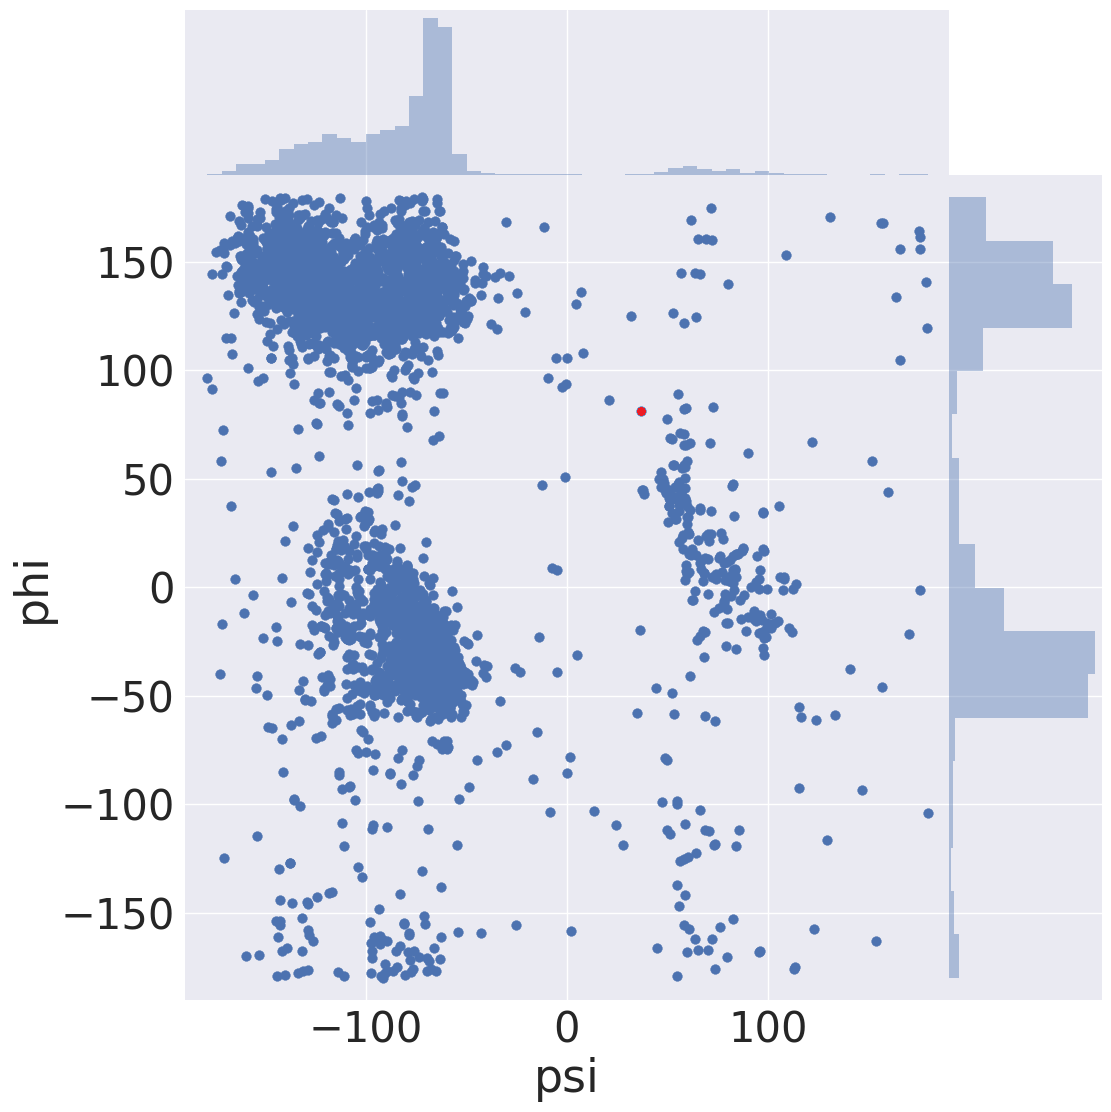
\includegraphics[width=.90\textwidth]{images/ramachandranplot_PF01287.png}
    \caption{Ramachandran Plot der Pfam PF01287. Auf der Abszisse sind die PSI und auf der Ordinate sind die PHI Winkel aufgetragen. Das Histogramm auf der Abszisse zeigt das Vorkommen der PSI Winkel, das Histogramm auf der Ordinate das Vorkommen der PHI Winkel. Der \ac{SNP} in der Aminosäuresequenz \texttt{1bkb} ist als roter Punkt dargestellt.}
    \label{fig:ramachandran_PF01287}
\end{figure}



\chapter{Diskussion}

In Kapitel \ref{sec:snp_auswertung} wurde gezeigt, dass \ac{SNP}s sich in Unterschieden in \ac{EP} ausdrücken. Nun soll diskutiert werden in wie fern sich \ac{SNP}s mittels \ac{EP}s annotieren lassen können.

\section{SNPs in Energieprofilen}
\label{sec:snps_in_eps}

\begin{figure}
    \centering
    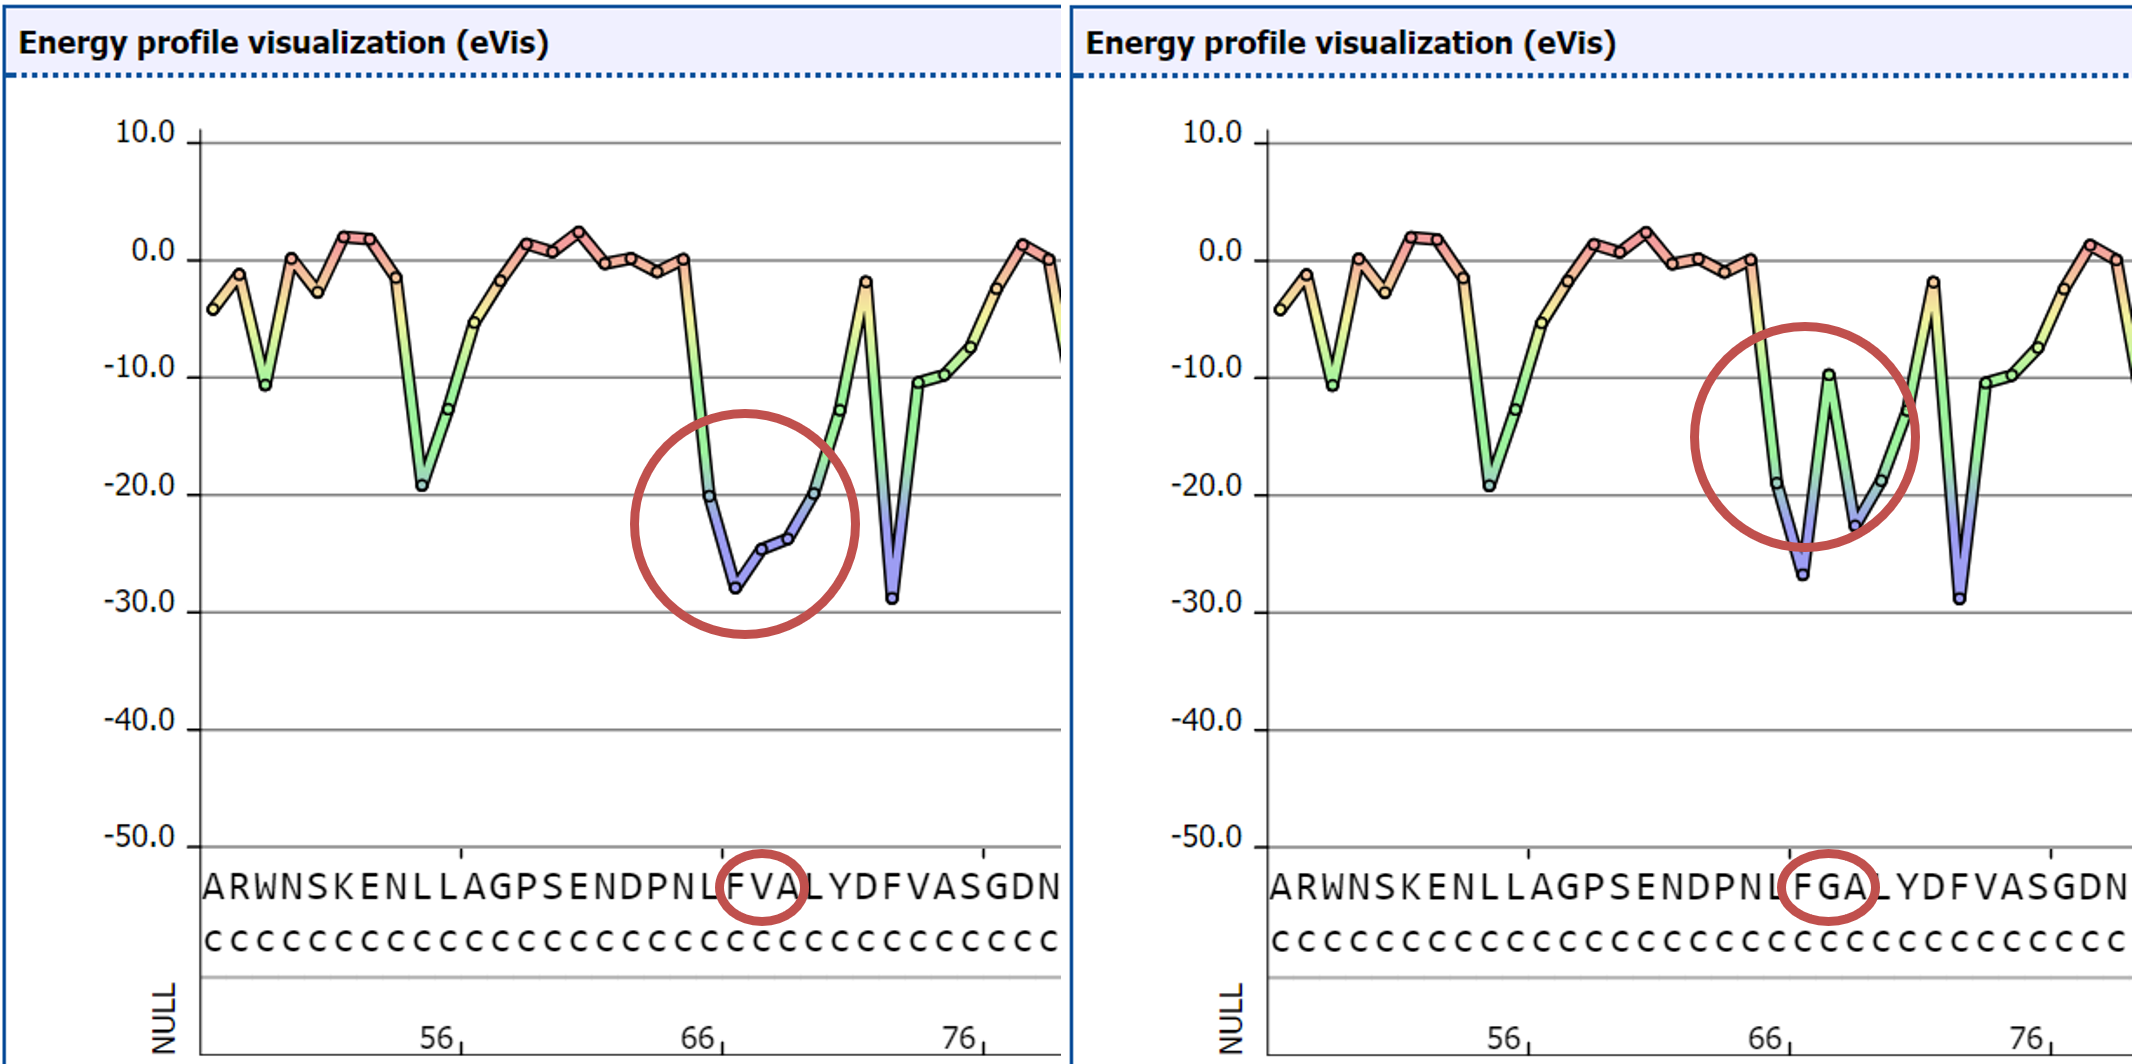
\includegraphics[width=.99\textwidth]{images/ep_vs_snp.png}
    \caption{\ac{eVis} Darstellung vom ePros Webserver (Kapitel \ref{sec:epros}) eines Ausschnittes eines \ac{EP}s. Die original Sequenz befindet sich links und Sequenz mit dem \ac{SNP}(rote Markierung) ist rechts. Auf der Abszisse sind die Aminosäuren im Einbuchstabencode aufgetragen, siehe Tabelle \ref{tab:amino_table}. Darunter ist die Sekundärstruktur als Buchstabencode und visualisiert aufgetragen. Unten ist die Aminosäureposition in 10er Schritten aufgetragen. Auf der Ordinate befinden sich die Energiewerte.}
    \label{fig:ep_vs_snp}
\end{figure}

Bei dem Vergleich von \ac{EP}s mit \ac{SNP} gegen das unmutierte \ac{EP} ist aufgefallen, dass sich die \ac{EP}s signifikant an den \ac{SNP} Positionen unterscheiden. Zum Verständnis ist ein \ac{EP} (mit und ohne \ac{SNP}) in \ac{Abb} \ref{fig:ep_vs_snp} dargestellt. Hier sieht man eine 2D Visualisierung eines \ac{EP}s, auf der Abszisse sind die Aminosäuren im Einbuchstabencode aufgetragen, wahrend auf der Ordinate die Energiewerte eingetragen sind. Die beiden Darstellungen unterscheiden sich nur durch die Substitution von Valin durch Glycin, so ist hier deutlich die Energiewert Differenz zwischen den beiden Darstellungen zu erkennen. So besitzt im Protein Valin an der Position 68 einen Energiewert von -25, der Glycin \ac{SNP} hingegen besitzt einen Energiewert von -10, so ergibt sich eine Delta von 15. 

Valin ist eine hydrophobe Aminosäure, während Glycin eine hydrophile Aminosäure ist, von daher ist es nicht überraschend, dass sich auch die Energiewerte des Proteins an dieser Stelle bei einem Austausch verändern. Dies zeigt uns deutlich, dass wir drastische Veränderungen der Proteinstruktur auch in den \ac{EP}s sehen.

Sieht man sich nun mit diesem Wissen \ac{Abb} \ref{fig:comp_plot_MSH2} an, so sieht man das der gutartige \ac{SNP} das \ac{EP} fast gar nicht verändert. Dies wird auch bestätigt, wenn man sich die chemischen Eigenschaften von Valin anschaut, denn Valin ist unpolar, genauso wie das Isoleucin welches es ersetzt hat. Zudem haben beide Aminosäuren in etwa die gleiche Größe. 

Generell sieht man das das \ac{EP} sich fast gar nicht verändert und die gesamte Energiedifferenz bei gerade mal -0,006 liegt. Dies passt alles sehr gut zu der ClinVar annotation, welche sagt das dieser \ac{SNP} gutartig ist.

Betrachten wir nun die untere \ac{Abb} in \ref{fig:comp_plot_MSH2}, so sehen wir, dass sich die Energie sich stark am \ac{SNP} verändert. Auch generell sieht man das sich die Energie im gesamten Protein viel stärker als im gutartigen \ac{SNP} in der oberen \ac{Abb} verändert. Wenn man sich die chemischen Eigenschaften von Glycin ansieht, sieht man das es polar ist, bei Tryptophan hingegen handelt es sich um eine unpolare Aminosäure. Zusätzlich ist Glycin die kleinste Aminosäure, während Tryptophan wesentlich größer ist. Auch dies passt gut zur ClinVar Annotation, welche besagt, dass es sich hierbei um ein pathogenes \ac{SNP} handelt.

Sehr ähnlich Verhält es sich mit der \ac{Abb} \ref{fig:comp_plot_ACADM}, hier ist im oben Bild ein gutartiges \ac{SNP} des Gens \texttt{ACADM} dargestellt. Hier sieht man wie in \ac{Abb} \ref{fig:comp_plot_MSH2} nur eine kleine Veränderung der Energie. Bei Methionin handelt es sich um eine hydrophobe Aminosäure genau wie bei Isoleucin, so scheint dieser \ac{SNP} chemisch keine große Veränderung zu machen. Diese Annahme wird auch von der ClinVar Annotation gutartig bestätigt. 

Sieht man sich hingegen das untere Bild an, so fällt eine sehr starke Veränderung des Energieniveaus am \ac{SNP} auf. Nach bisherigem wissen würden wir diesen \ac{SNP} also als pathogen einordnen, dies ist richtig, wenn man die ClinVar Annotation hinzuzieht. Auch die chemischen Eigenschaften der Threonin unterscheiden sich von den der Aminosäure Isoleucin, denn Threonin ist polar und Isoleucin nicht. 



\section{Anwendbarkeit der EPs zur Annotation von SNPs im Panel}

In Kapitel \ref{sec:snps_in_eps} wurde gezeigt, dass es möglich ist Energieprofile zu nutzen um \ac{SNP}s zu annotieren.  Die Auswertung der \ac{SNP}s aus Tabelle \ref{tab:snps_memb} und \ref{tab:snps_glob} ergab, dass dies Möglich ist und ein MCC von 0,8 für globuläre und sogar 1,0 für Membran assozierte Proteine erreicht werden kann. Doch jetzt stellt sich die Frage, ob wir die Erkenntnisse der Arbeit nutzen können um die im Illumina TruSight Myeloid Sequencing Panel auftretenden Gene zu annotieren. 

Dafür wurde zuerst versucht per Hand die einzelnen Gen Sequenzen herunterzuladen und anschließend in Swissmodel zu modellieren. Doch leider lieferte dies nicht die gewünschten Ergebnisse, die Coverage war in den meisten Fällen sehr schlecht. So bewegte sich z.B. die Coverage für \texttt{NRAS} zwischen 1-4\%, sodass nur einzelne Helices abgedeckt waren. Dieses Bild zeigte sich so, oder so ähnlich für alle getesteten Proteine. 

\begin{table}[]
    \centering
    \caption{Illumina TruSight Myeloid Sequencing Panel Gene \emph{coverage}, Transkriptlänge ist mit UTRs und CDS angegeben.}
    \label{tab:illumina_coverage}
    \resizebox{\linewidth}{!}{%
    \begin{tabular}{lllll}
    \hline
    \multicolumn{1}{|l|}{Genname} & \multicolumn{1}{l|}{Genlänge (bp)} & \multicolumn{1}{l|}{Transkriptlänge} & \multicolumn{1}{l|}{PDB-ENSP} & \multicolumn{1}{l|}{PDB Coverage} \\ \hline
    IDH1 & 29847 & 2298 & 1t09.A & 17,97\% \\
    KDM6A & 239425 & 5438 & 3avr.A & 9,58\% \\
    JAK2 & 143793 & 5285 & 4z32.A & 9,18\% \\
    NRAS & 12425 & 4449 & 3con.A & 3,84\% \\
    RAD21 & 28931 & 3749 & 4pju.B & 3,71\% \\
    NOTCH1 & 51418 & 9371 & 3eto.A & 3,06\% \\
    \end{tabular}}
\end{table}

Aus diesem Grund wurde der EnsemblBioMart\footnote{\url{https://www.ensembl.org/biomart}} hinzugezogen, dieser ermöglicht es dem Nutzer leicht spezielle Datensätze mit verschiedensten Filtern herunter zu laden. So wurde in diesem Fall die Genliste des Illumina Panels mit 54 Genen im BioMart eingefügt und Genlänge, Transkriptlänge, korrespondierende \ac{PDB} Einträge und deren Start und Stopp Position abgefragt, dargestellt in Tabelle \ref{tab:illumina_coverage}. Die Start und Stopp Position der \ac{PDB} Einträge wurde mit der Transkriptlänge verrechnet, so dass eine prozentuale Coverage abgebildet werden kann. Wie zu sehen ist, besitzt \texttt{IDH1} die beste Coverage mit 17,97\%, dies ist leider viel zu wenig um eine erfolgreiche Berechnung eines \ac{EP}s durchzuführen. Bei den anderen Genen sieht es leider noch schlechter aus, denn von den 54 Genen im Panel weisen gerade mal 6 Gene überhaupt eine Teilabdeckung auf. 

\begin{table}[]
    \centering
    \caption{VariantPlex Solid Tumor Kit Coverage, Transkriptlänge ist mit UTRs und CDS angegeben.}
    \label{tab:variantplex_coverage}
    \resizebox{\linewidth}{!}{%
    \begin{tabular}{lllll}
    \hline
    \multicolumn{1}{|l|}{Genname} & \multicolumn{1}{l|}{Genlänge (bp)} & \multicolumn{1}{l|}{Transkriptlänge} & \multicolumn{1}{l|}{PDB-ENSP} & \multicolumn{1}{l|}{Coverage} \\ \hline
    ATM & 146618 & 12954 & 5np0.A & 23,58\% \\
    IDH1 & 29847 & 2298 & 1t09.A & 17,97\% \\
    H3F3A & 10150 & 799 & 3av2.A & 16,90\% \\
    RB1 & 178235 & 4840 & 4elj.A & 15,17\% \\
    BRAF & 205437 & 2480 & 4mnf.A & 12,26\% \\
    PIK3CA & 91979 & 9093 & 2rd0.A & 11,73\% \\
    SMO & 24673 & 3738 & 5v56.A & 10,27\% \\
    RHOA & 53853 & 2031 & 1ftn.A & 9,45\% \\
    JAK2 & 143793 & 5285 & 4z32.A & 9,18\% \\
    CCND1 & 13387 & 4307 & 2w96.A & 6,27\% \\
    ALK & 728792 & 6220 & 4fob.A & 5,66\% \\
    DDR2 & 156027 & 3096 & 2wuh.A & 5,43\% \\
    ROS1 & 137555 & 7435 & 3zbf.A & 4,01\% \\
    SMAD4 & 56651 & 8495 & 1dd1.A & 3,14\% \\
    NOTCH1 & 51418 & 9371 & 3eto.A & 3,06\% \\
    MYCN & 6443 & 2602 & 5g1x.B & 2,34\%
    \end{tabular}}
\end{table}

Um zu überprüfen, ob es sich bei dem Illumina Panel nicht um eine unglückliche Ausnahme handelt wurde noch ein zweites Panel überprüft. Das \emph{VariantPlex Solid Tumor Kit}\footnote{\url{http://archerdx.com/variantplex/solid-tumor}} umfasst 67 Gene im Zusammenhang mit soliden Tumoren. Doch auch hier ist nur ein Bruchteil der Gene aufgeklärt und von diesen 16 Genen, ist keines komplett strukturell aufgeklärt. Die höchste Coverage hat \texttt{ATM} mit 23,58\%, dies ist jedoch immer noch zu wenig um damit eine Homologie Modellierung durchzuführen. Auch dieses Panel beinhaltet \texttt{IDH1} und weist damit ebenfalls eine Coverage von 17,97\% auf gefolgt von \texttt{H3F3A} mit einer Coverage von 16,90\%. Bei den restlichen Treffern fällt die Coverage stark ab.

Somit lässt sich abschließend sagen, dass sich \ac{APs} (noch) nicht für die Annotation von \ac{SNP}s im Illumina TruSight Myeloid Sequencing Panel eignen, da einfach noch zu wenige Strukturen aufgeklärt sind. Denn ohne aufgeklärte Struktur macht es keinen Sinn ein Homologie Berechnung durchzuführen, denn wie in \ref{sec:min_coverage} gezeigt, würde das Ergebnis unbrauchbar sein. Sodass keine \ac{EP} Berechnung durchgeführt werden kann. 


\subsection{Minimale Coverage und Sequenzidentität}
\label{sec:min_coverage}

In diesem Abschnitt wird diskutiert, welche minimale Coverge ein Proteine haben muss damit es Sinn macht ein \ac{EP} dafür zu berechnen. Denn es hat sich herausgestellt das die Vorhersage eines \ac{SNP}s sehr stark abhängig von dem Template ist.

\begin{figure}
    \centering
    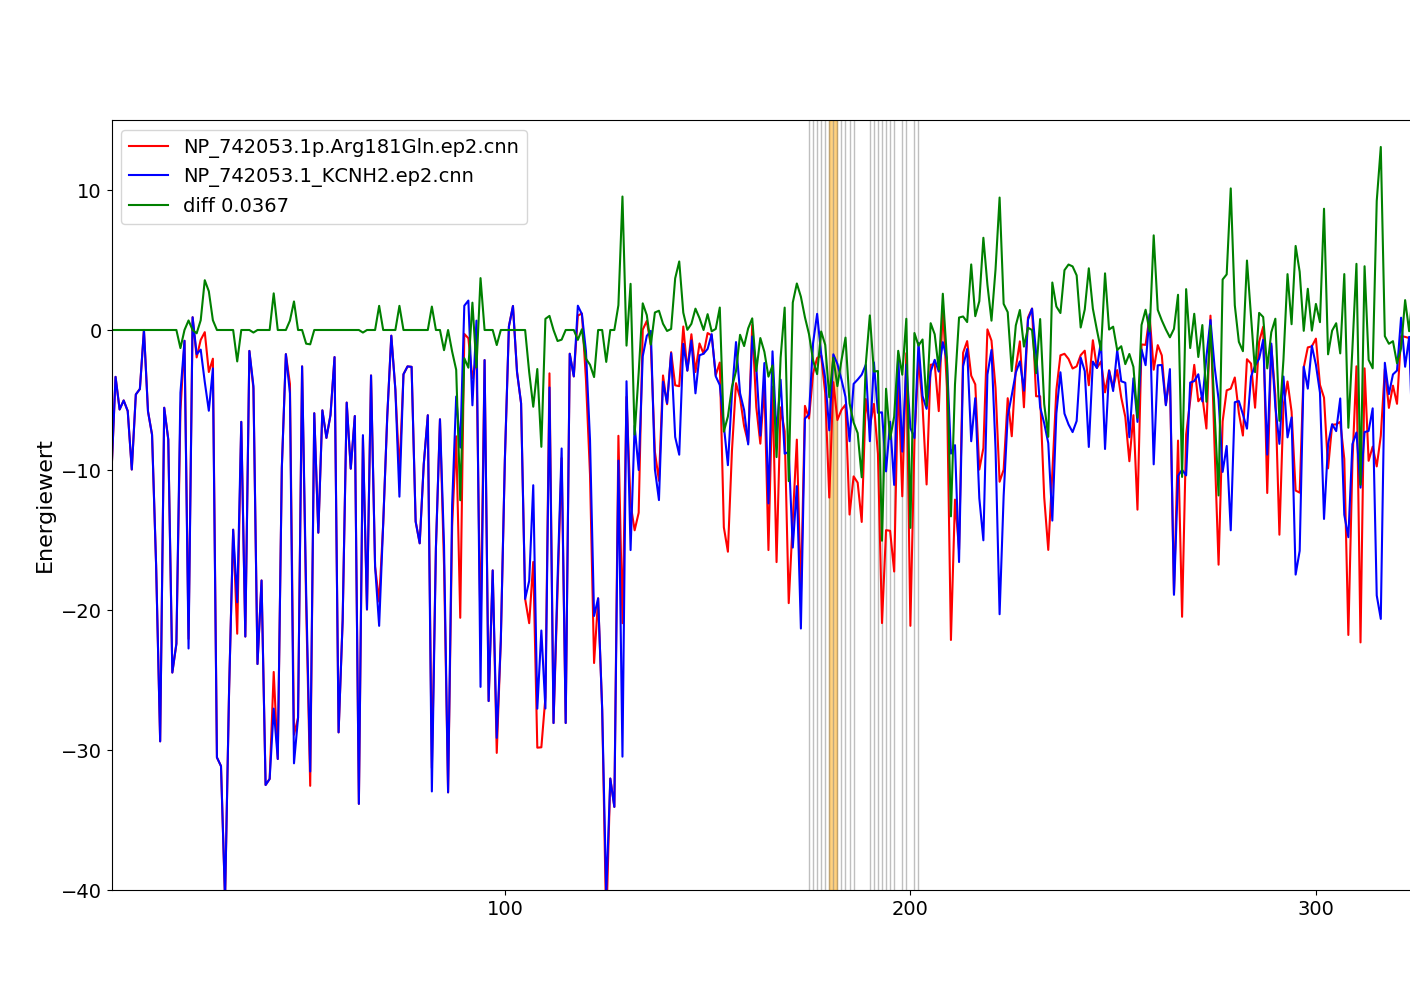
\includegraphics[width=.99\textwidth]{images/comp_plot_KCNH2_Arg181Gln.png}
    \caption{Fehlerhafter Plot, eigentlich benign ist aber jenseits von gut und böse}
    \label{fig:fail_ep}
\end{figure}


%- Überprüfen ob Sequenz identität wichtig ist? 



\subsection{Problem mit dem Datensatz}
- Warum ist keien perfekte Trennung der SNPs möglich?

- Fehler im Modell

- Gesamter Ansatz
- ClinVar hat nicht die Warheit

- Mutations an sich ist nicht benign
- Fehlende zusatzdaten -> wird aufgehoben ?
- Patienten alter, und co

- Problem zu wenige benign SNPs
- 


Entweder Protein vollständig aufgeklärt, wie \url{ABCG2} \url{https://www.ncbi.nlm.nih.gov/pubmed/?term=28554189} oder \texttt{KCNH2} \url{http://www.rcsb.org/pdb/explore/explore.do?structureId=5VA1} aber dafür keine mehrfach bestätigten SNPs, oder viele mehrfachbestätige SNPs, jedoch keine vollständige 3D Struktur, siehe...

SNPs liegen nicht in der aufgeklärten 3S Struktur, siehe ...

SNPs liegen auf verschiedenen Transkripten ...

Sequenz Identität ist nicht ausreichend, siehe ...

Noch nicht ausreichend 3D Strukturen:

Die Anzahl aufgeklärter 3D Strukturen liegt bei XX\% bei einem Wachstum von XX, hingegen die 3D Strukturen nur XX\% bei einem Wachstum von XX\%. Sodass es im Jahr XXYY XY\% zu erwarten sind * Quelle: "Trends in structural coverage of the protein universe and the impact of the Protein Structure Initiative"


UniProtKB/Swiss-Prot enthält seit dem 22. Juli 2008 etwa 400K-Sequenzeinträge, während die Protein-Datenbank (PDB) nur etwas mehr als 50K experimentell bestimmte Proteinstrukturen enthält. 
Quelle (An integrated database for complex protein structure modeling) Aus <http://ieeexplore.ieee.org/document/4686206/?reload=true> 
Heute:  
555.426 sequence entries Aus \url{http://web.expasy.org/docs/relnotes/relstat.html} 
133.589 Biological Macromolecular Structures aus \url{https://www.rcsb.org/pdb/statistics/contentGrowthChart.do?content=total&seqid=100}

Wobei nur einige PDB Einträge nur Subdomänen von Proteinen sind
Ein PDB Eintrag =/= Eine komplette Squenz

Das gilt für alle Strukturen über alle Spezies, für den Homo Sapiens gibt es also nur ein Teilsatz an 3D Strukturen.
    >Wie viele Gene hat der Mensch? >
    "29 000. Die ungefähre Lokalisation von 22 000 Genen ist bereits bekannt."
Aus \url{https://www.deutsche-apotheker-zeitung.de/daz-az/2001/daz-11-2001/uid-389}

"Each of the estimated 30,000 genes in the human genome makes an average of three proteins."
Aus \url{https://www.genome.gov/11006943/human-genome-project-completion-frequently-asked-questions/}







%\section{Ramachandran Diskussion}

%Winkelveränderung
%- In der Mutation
%- In den Kontakten




zusätzliches

nicht alle Aminosäuren im gleichen Energiespektrum zu finden sind.
\chapter{Ausblick}



\section{Kryo-Elektronenmikroskopie}

In dieser Arbeit wurde mit einem relativ kleinen Datensatz an \ac{SNP}s gearbeitet, die Gründe dafür wurden in Kapitel \ref{sec:probleme_mit_dem_datensatz} diskutiert. Als Hauptgrund hat sich herausgestellt, dass es einfach an der Tatsache liegt, dass zu wenige 3D Strukturen aufgeklärt sind. 

Die Anzahl aller strukturell aufgeklärten Proteine hat sich in den letzten 10 Jahren von 30\% auf 40\% erhöht, im Gegensatz dazu hat sich die Anzahl an bekannten Sequenzen exponentiell vervielfacht. Basierend auf den aktuellen Trends wird erwartet, dass 55\% der strukturellen Abdeckung innerhalb von 15 Jahren erreicht wird \cite{Khafizov.2014}.

Die neusten Entwicklungen in der Chemie, lassen jedoch hoffen, dass in Zukunft zu erwarten ist, dass sehr viel mehr und vor allem hochauflösende 3D Strukturen zu Verfügung stehen. Denn der diesjährige (2017) Nobelpreis in Chemie\footnote{\url{https://www.nobelprize.org/nobel_prizes/chemistry/laureates/2017/announcement.html}
}, mit dem Titel:
\begin{quote}
    ''Für die Entwicklung der Kryo-Elektronenmikroskopie, für die hochauflösende Strukturbestimmung von Biomolekülen in Lösungen.''
\end{quote}
Von Jacques Dubochet, Joachim Frank und Richard Henderson, beschäftigt sich genau mit diesem Thema. So haben die Herren erfolgreich gezeigt, dass es möglich ist die 3D Struktur hochauflösend mit einem Kryo-Elektronenmikroskop in der Zelle zu bestimmen.

\begin{figure}
    \centering
    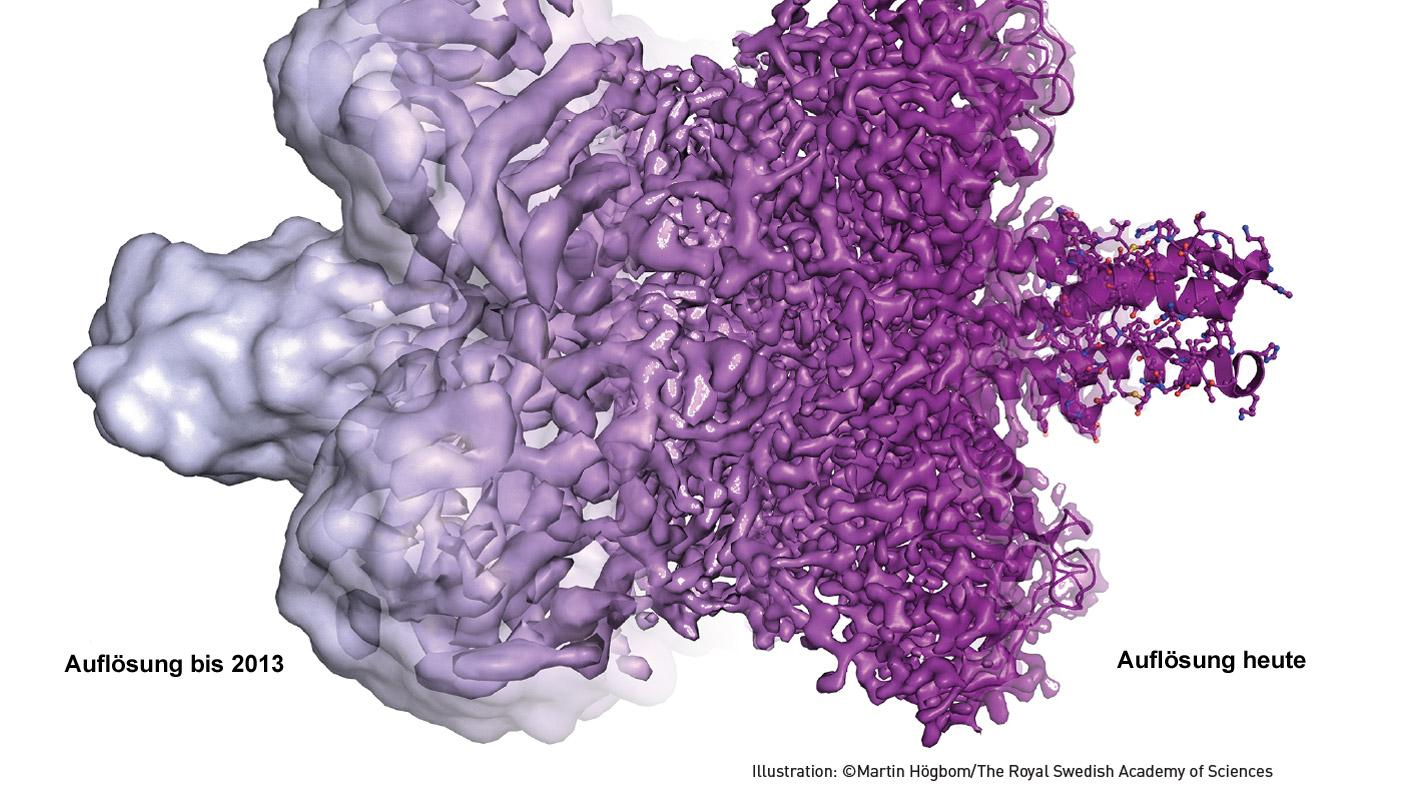
\includegraphics[width=.95\textwidth]{images/Verbesserung_der_Aufloesung.jpg}
    \caption{Verbesserung der Auflösung von 2013 bis heute 2017\protect\footnotemark{}.}
    \label{fig:verbesserte_aufloesung}
\end{figure}

Bisher war es notwendig das Protein aufzureinigen um es anschließend in Kristallform zu bringen, da die Röntgenstrukturanalyse nur kristalline Strukturen aufklären kann. 

Die Qualität solcher Strukturen hängt von der Auflösung ab, diese liegt bei 6 bis 2 Angström, das ist links in \ac{Abb} \ref{fig:verbesserte_aufloesung} zu sehen. Die neue Methode ermöglicht es die Strukturen deutlich detailierter darzustellen, wie rechts in der \ac{Abb} gezeigt.

\begin{quote}
    ''Now there's an explosion in research''
    - Peter Brzezinski
\end{quote}

Zusätzlich lassen sich so erstmals Interaktionen zwischen Proteinen direkt unter dem Mikroskop erkennen. Damit kann man auch Proteine in ihren verschiedenen Zuständen beobachten. Das ist auch sehr interessant für diese Arbeit, denn so könnten Energieveränderungen in verschiedenen Konformationen betrachtet werden.
\footnotetext{\url{http://www.blopig.com/blog/wp-content/uploads/2014/04/CootLigand2-624x349.png}}

%" Eine physikalisch korrekte Darstellung molekularer Strukturen erfolgt über die Elektronendichte, welche eine realistische Abbildung des Moleküls in der Realität ist."

%\begin{figure}
%    \centering
%    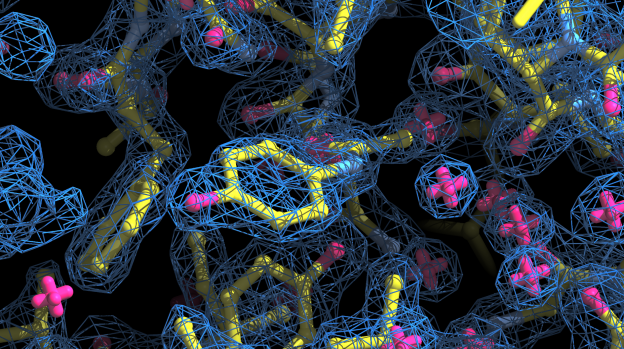
\includegraphics[width=.95\textwidth]{images/approximation.png}
%    \caption{Dargestellt ist eine Approximation der Atome eines Proteins.}
%   \label{fig:approximation}
%end{figure}



\section{Anwendungsgebiete}

Sollten genug 3D Strukturen zu Verfügung stehen, so sollte es möglich sein alle \ac{SNP}s im Illumina Panel zu annotieren. Generell ist die Annotation mittels \ac{EP}s nicht auf das Illumina Panel begrenzt, so sollte es möglich sein alle \ac{SNP}s zu annotieren

Wie in Kapitel \ref{sec:leuk} gezeigt, ist die 5 Jahres Überlebensrate nicht besonders hoch, da die Rückfall Quote nach der Remission sehr hoch ist. 

Um diesen Rückfall rechtzeitig zu erkennen, ist es denkbar nach der Remission spezielle Patienten spezifische pathogene \ac{SNP}s, in regelmäßigen Abständen, im Blut zu suchen. So könnte man früher intervenieren und somit den Rückfall aufhalten, bevor der Patient wieder unter den Symptomen der \ac{AML} leidet.
%\ac{MDS}
Diese \ac{SNP}s im Blut, lassen sich schon in sehr geringer Konzentration nachweisen, noch bevor der Patient wieder die typischen Symptome zeigt. So spricht man auch von personalisierter Medizin, da das \ac{SNP} Profil für jeden Patienten anders aussehen würde.




\section{Zusammenfassung}

% Konstruktion des Datensatzes

% SNP Auswahl

In dieser Arbeit wurde gezeigt, dass sich \acf{APs} zum Annotieren von \acf{SNP}s in Proteinen eignen. Dafür wurden Proteine mit aufgeklärter 3D Struktur untersucht, indem die Aminosäuresequenz mit \ac{SNP}s mutiert wurde. Danach wurden die 3D Strukturen, der mutierten Sequenzen zusammen mit der Referenzsequenz, mittels Homologie Modellierung ermittelt. Für diese Strukturen wurden anschließend \acf{EP} errechnet, welche danach verglichen wurden.

Dieser Vergleich hat ergeben, dass verschiedene \ac{SNP}s sich unterschiedlich auf das Energieniveau im \ac{EP} auswirken. Des weiteren wurde gezeigt, dass pathogene \ac{SNP}s deutlich weiter 

Nach verschiedenen Klassifizierungsansätzen, wurde gezeigt, dass es am sinnvollsten ist globuläre und alpha helicale Membranproteine getrennt zu betrachten. 

Globuläre Proteine wurden nach der totalen Differenz des Energiewertes am \ac{SNP} klassifiziert. So wurde ein MCC von 0,8 ermittelt, wenn die untere Grenze auf 2 und die obere Grenze auf 7 festgesetzt wird. 

Membran assoziierte Proteine wurden nach der Differenz des Energiewertes am \ac{SNP} klassifiziert, hierbei wurde die untere Grenze auf -2,5 und die obere Grenze auf -0,3 festgelegt. Sind die Werte nun unter oder Über dieser Grenze, ist anzunehmen, dass es sich um ein pathogenen \ac{SNP} handelt. Hiermit wurde ein MCC von 1 errechnet, allerdings ist anzumerken, dass der Datensatz relativ klein ist.

Generell lässt sich festhalten das momentan noch zu wenige 3D Strukturen von Proteinen aufgeklärt sind, dies ist auch der Grund warum mit diesem Ansatz keine \ac{AML} assoziierten \ac{SNP}s aus dem Illumina TruSeq Myeloid Sequenzing Panel annotiert werden können.

Dies wird sich jedoch in den nächsten Jahren ändern, da z.B. der diesjährige Nobelpreis in Chemie für die Entwicklung der Kryo-Elektronenmikroskopie für die hochauflösende Strukturbestimmung von Biomolekülen in Lösungen ausgeschrieben wurde. Damit ist es möglich schneller und günstiger hochauflösende 3D Strukturen zu erfassen, als es bisher der Fall war.



\section{Weiterführende Arbeit}

einzelnes Protein zur Bestätigung
aufgeklärte muta + bakterium rodhopsin

Online Service hosten


Das Programm eignet sich als Basismodul für eine klinisch Anayse-Pipeline die der eigentlichen variantenanalyse nachgeschaltet ist
\chapter[Schlussbemerkungen]%
        {Schlussbemerkungen%
        \protect\footnote{Diese Anmerkung dient nur dazu, die (in seltenen Fällen sinnvolle)
				Verwendung von Fußnoten bei Überschriften zu demonstrieren.}}%
\label{cha:Schluss}

An dieser Stelle sollte eine Zusammenfassung der Diplomarbeit
stehen, in der auch auf den Entstehungsprozess, persönliche
Erfahrungen, Probleme bei der Durchführung,
Verbesserungsmöglichkeiten, mögliche %
Erweiterungen \usw\ eingegangen werden kann. War das Thema richtig
gewählt, was wurde konkret erreicht, welche Punkte blieben offen
und wie könnte man von hier aus weiter arbeiten?


\section{Lesen und lesen lassen}

Wenn die Arbeit fertig ist, sollten Sie diese zunächst selbst nochmals vollständig und sorgfältig durchlesen, auch wenn man vielleicht das mühsam entstandene Produkt längst nicht mehr sehen möchte. Zusätzlich ist sehr zu empfehlen, auch einer weiteren Person diese Arbeit anzutun -- man wird erstaunt sein, wieviele Fehler man selbst überlesen hat. 



\section{Checkliste}

Abschließend noch eine kurze Liste der wichtigsten Punkte, an denen erfahrungsgemäß die häufigsten Fehler auftreten (Tab.\ \ref{tab:checkliste}).


\begin{table}
\caption{Checkliste. Diese Punkte bilden auch die Grundlage der routine\-mäßigen Formbegutachtung in Hagenberg.}
\label{tab:checkliste}
\centering
\fbox{
\begin{minipage}{0.95\textwidth}
\medskip
\begin{itemize}
	\item[$\Box$] \textbf{Titelseite:} Länge des Titels (Zeilenumbrüche), Name, Studiengang, Datum.
	\item[$\Box$] \textbf{Erklärung:} vollständig Unterschrift.
	\item[$\Box$] \textbf{Inhaltsverzeichnis:} balanzierte Struktur, Tiefe, Länge der Überschriften.
	\item[$\Box$] \textbf{Kurzfassung/Abstract:} präzise Zusammenfassung, Länge, gleiche Inhalte.
	\item[$\Box$] \textbf{Überschriften:} Länge, Stil, Aussagekraft.
	\item[$\Box$] \textbf{Typographie:} sauberes Schriftbild, keine "`manuellen"' Abstände zwischen Absätzen oder Einrückungen, keine überlangen Zeilen, Hervorhebungen, Schriftgröße, Platzierung von Fußnoten.
	\item[$\Box$] \textbf{Punktuation:} Binde- und Gedankenstriche richtig gesetzt, Abstände nach Punkten (\va\ nach Abküzungen).
	\item[$\Box$] \textbf{Abbildungen:} Qualität der Grafiken und Bilder, Schriftgröße und -typ in Abbildungen, Platzierung von Abbildungen und Tabellen, Captions. Sind \emph{alle} Abbildungen (und Tabellen) im Text referenziert?
	\item[$\Box$] \textbf{Gleichungen/Formeln:} mathem.\ Elemente auch im Fließtext richtig gesetzt, explizite Gleichungen richtig verwendet, Verwendung von mathem.\ Symbolen.
	\item[$\Box$] \textbf{Quellenangaben:} Zitate richtig referenziert, Seiten- oder Kapitelangaben.
	\item[$\Box$] \textbf{Literaturverzeichnis:} mehrfach zitierte Quellen nur einmal angeführt, Art der Publikation muss in jedem Fall klar sein, konsistente Einträge, Online-Quellen (URLs) sauber angeführt.
	\item[$\Box$] \textbf{Sonstiges:} ungültige Querverweise (\textbf{??}), Anhang, Papiergröße der PDF-Datei (A4 = $8.27 \times 11.69$ Zoll), Druckgröße und -qualität.
\end{itemize}
\medskip
\end{minipage}%
}
\end{table}




%%%----------------------------------------------------------
%%%Anhang
\appendix
\chapter*{DVD}



\begin{center}
{\Large DVD mit Anhang}

\bigskip

\Messbox{120}{120} % Angabe der Breite/Hoehe in mm

\bigskip

Der gleiche Inhalt der DVD befindet sich unter folgender Adresse:
\url{https://www.dropbox.com/sh/llvj4kf6lwykkz2/AABxlTitVyJIBpt3217Y8bFza?dl=0}

Der Quellcode und die Skripte sind zudem im GitHub zu finden:
\url{https://github.com/TobiasJu}

\end{center}


%%%----------------------------------------------------------
%\MakeBibliography
\printbibliography  % für natbib
%%%----------------------------------------------------------

%%%Messbox zur Druckkontrolle
\chapter*{Messbox zur Druckkontrolle}



\begin{center}
{\Large --- Druckgröße kontrollieren! ---}

\bigskip

\Messbox{100}{50} % Angabe der Breite/Hoehe in mm

\bigskip

{\Large --- Diese Seite nach dem Druck entfernen! ---}

\end{center}



\end{document}
